%  LaTeX support: latex@mdpi.com 
%  In case you need support, please attach all files that are necessary for compiling as well as the log file, and specify the details of your LaTeX setup (which operating system and LaTeX version / tools you are using).

%=================================================================
\documentclass[energies,article,submit,moreauthors,pdftex]{Definitions/mdpi} 

\usepackage{graphicx}
\usepackage{subfig}
\usepackage{subcaption}
% If you would like to post an early version of this manuscript as a preprint, you may use preprint as the journal and change 'submit' to 'accept'. The document class line would be, e.g., \documentclass[preprints,article,accept,moreauthors,pdftex]{mdpi}. This is especially recommended for submission to arXiv, where line numbers should be removed before posting. For preprints.org, the editorial staff will make this change immediately prior to posting.



%---------
% article
%---------
% The default type of manuscript is "article", but can be replaced by: 
% abstract, addendum, article, benchmark, book, bookreview, briefreport, casereport, changes, comment, commentary, communication, conceptpaper, conferenceproceedings, correction, conferencereport, expressionofconcern, extendedabstract, meetingreport, creative, datadescriptor, discussion, editorial, essay, erratum, hypothesis, interestingimages, letter, meetingreport, newbookreceived, obituary, opinion, projectreport, reply, retraction, review, perspective, protocol, shortnote, supfile, technicalnote, viewpoint
% supfile = supplementary materials

%----------
% submit
%----------
% The class option "submit" will be changed to "accept" by the Editorial Office when the paper is accepted. This will only make changes to the frontpage (e.g., the logo of the journal will get visible), the headings, and the copyright information. Also, line numbering will be removed. Journal info and pagination for accepted papers will also be assigned by the Editorial Office.

%------------------
% moreauthors
%------------------
% If there is only one author the class option oneauthor should be used. Otherwise use the class option moreauthors.

%---------
% pdftex
%---------
% The option pdftex is for use with pdfLaTeX. If eps figures are used, remove the option pdftex and use LaTeX and dvi2pdf.

%=================================================================
\firstpage{1} 
\makeatletter 
\setcounter{page}{\@firstpage} 
\makeatother
\pubvolume{xx}
\issuenum{1}
\articlenumber{5}
\pubyear{2020}
\copyrightyear{2020}
%\externaleditor{Academic Editor: name}
\history{Received: date; Accepted: date; Published: date}
%\updates{yes} % If there is an update available, un-comment this line

%% MDPI internal command: uncomment if new journal that already uses continuous page numbers 
%\continuouspages{yes}

%=================================================================
% Add packages and commands here. The following packages are loaded in our class file: fontenc, calc, indentfirst, fancyhdr, graphicx, lastpage, ifthen, lineno, float, amsmath, setspace, enumitem, mathpazo, booktabs, titlesec, etoolbox, amsthm, hyphenat, natbib, hyperref, footmisc, geometry, caption, url, mdframed, tabto, soul, multirow, microtype, tikz

%=================================================================
%% Please use the following mathematics environments: Theorem, Lemma, Corollary, Proposition, Characterization, Property, Problem, Example, ExamplesandDefinitions, Hypothesis, Remark, Definition, Notation, Assumption
%% For proofs, please use the proof environment (the amsthm package is loaded by the MDPI class).

%===============================================================
%                           TITLE & AUTHORS
%===============================================================
% Full title of the paper (Capitalized)
\Title{Impact of the COVID-19 Lockdown on Electricity System in Great Britain: a Study on Energy Demand, Generation, Pricing and Grid Stability}

% Author Orchid ID: enter ID or remove command
\newcommand{\orcidauthorA}{0000-0001-7596-0944} % Add \orcidA{} behind the author's name
\newcommand{\orcidauthorB}{0000-0002-3494-0469} % Add \orcidB{} behind the author's name

% Authors, for the paper (add full first names)
\Author{Desen Kirli $^{1,*,}$\orcidA{}, Maximilian Parzen $^{1}$ and Aristides Kiprakis $^{1,}$\orcidB{}}

% Authors, for metadata in PDF
\AuthorNames{Firstname Lastname, Firstname Lastname and Firstname Lastname}

% Affiliations / Addresses (Add [1] after \address if there is only one affiliation.)
\address{%
$^{1}$ \quad Institute for Energy Systems, School of Engineering, University of Edinburgh\\}
% $^{2}$ \quad Affiliation 2; e-mail@e-mail.com}

% Contact information of the corresponding author
\corres{Correspondence: desen.kirli@ed.ac.uk}
%; Tel.: (optional; include country code; if there are multiple corresponding authors, add author initials) +xx-xxxx-xxx-xxxx (F.L.)

% Current address and/or shared authorship
% \firstnote{Current address: Affiliation 3} 
% \secondnote{These authors contributed equally to this work.}
% The commands \thirdnote{} till \eighthnote{} are available for further notes


%===============================================================
%                           ABSTRACT & KEYWORDS
%===============================================================

% Abstract (Do not insert blank lines, i.e. \\) 
\abstract{
%Electricity is both a vital service and necessity at all times yet even more critical during a pandemic. 
The outbreak of SARS-COV-2 disease 2019 (COVID-19) abruptly changed the patterns in electricity consumption, challenging the system operations of forecasting and balancing the supply and demand. This is due to the mitigation measures that include lockdown and Work from Home (WFH) which decreased the aggregated demand and altered its profile remarkably. In this paper, we characterise these changes with various quantitative markers and compare it with pre-COVID-19 business-as-usual data using the case study of Great Britain. The ripple effects on the generation portfolio, system frequency, accuracy of forecasting and imbalance pricing are also analysed. An energy data extraction and pre-processing pipeline that can be used in a variety of similar studies is also presented.}
%  Electricity is both a vital service and necessity at all times yet even more critical during a pandemic. The ongoing outbreak of coronavirus disease 2019 (COVID-19) has abruptly changed the patterns in electricity consumption, challenging the system operators who forecast and match the electricity supply and demand. This is due to the mitigation measures that include self-isolation, lockdown and working remotely which decreased the aggregated demand and altered its profile remarkably. In this paper, we characterise the changes in the demand profile with various quantitative markers and compare it with pre-COVID-19 business-as-usual data using the case study of Great Britain. The impact on the generation portfolio and pricing is also analysed using the value factor method. We present a timeline of the pandemic mitigation actions taken and the corresponding changes in the demand profile and energy portfolio. The volume of demand-side response services is also analysed against the historic data that shows (?) an increase. ?maybe include frequency services and comment on it as a grid stability measure? + the main conclusions or interpretations - once we have them :)

% A single paragraph of about 200 words maximum. For research articles, abstracts should give a pertinent overview of the work. We strongly encourage authors to use the following style of structured abstracts, but without headings: (1) Background: Place the question addressed in a broad context and highlight the purpose of the study; (2) Methods: Describe briefly the main methods or treatments applied; (3) Results: Summarize the article's main findings; and (4) Conclusion: Indicate the main conclusions or interpretations. The abstract should be an objective representation of the article, it must not contain results which are not presented and substantiated in the main text and should not exaggerate the main conclusions

% Keywords (list 3 to 10 pertinent keywords specific to the article, yet reasonably common within the subject discipline.
\keyword{electricity system, COVID-19, electricity demand, demand-side response}


%===============================================================
%                           MAIN TEXT
%===============================================================

\begin{document}
\tableofcontents
%===============================================================
%                           INTRO
%===============================================================
% \textbf{***ENERGIES -SPECIAL ISSUES ON COVID-19***}

% (1) \textbf{Special Issue COVID-19 Pandemics: Energy, Economic, Environmental, Social, Policy and Health Impacts}
% \url{https://www.mdpi.com/journal/energies/special\_issues/covid\_energy\_economic\_environmental\_social\_policy\_health}


% (2) \textbf{Special Issue Coronavirus Crisis, Energy Markets and Policies and Their Macro-Financial Implications}
% \url{https://www.mdpi.com/journal/energies/special_issues/Coronavirus_Crisis_Energy_Markets_Policies_Their_Macro_Financial_Implications}




% \textcolor{blue}{\textbf{***SIMILAR ANALYSIS - COVID-19 \& Elect Demand***}}

% (1) \textbf{UKERC Report: Electricity demand during week one of COVID-19 lockdown}
% \url{http://www.ukerc.ac.uk/news/covid-lockdown-electricity-demand.html}

% (2) \textbf{EPRI Report: COVID-19 Bulk System Impacts Demand Impacts and Operational and Control Centers}
% \url{http://mydocs.epri.com/docs/public/covid19/3002018602R2.pdf}

% (3) \textbf{Aurora Report: Impact of Coronavirus on European energy markets}
% \url{https://www.auroraer.com/wp-content/uploads/2020/04/Aurora-COVID-19-weekly-impact-tracker-090420-.pdf}

% (4) \textbf{HIGHEST SYSTEM PRICE SINCE}
% \url{https://www.elexon.co.uk/article/elexon-insight-highest-system-price-in-19-years/}

% (5) \textbf{The 'lockdown effect' on TV viewing habits and the electricity grid}
% \url{https://www.nationalgrideso.com/news/lockdown-effect-tv-viewing-habits-and-electricity-grid}


% (6) \textbf{NEW UN REPORT ON THE COVID-19 IMPACT ON THE SDG - includes low-carbon generation goals.}
% \url{bit.ly/2WZI3I4}


% \url{https://www.elexon.co.uk/article/coronavirus-temporary-derogations-to-improve-settlement-accuracy/}

\section{Introduction}

% Electricity is a vital service at all times. In the UK, the utilities sector was identified as critical for the continuation of essential public services by the government. As it is essential to meet the heat and lighting demand for 
% homes, businesses to function and for the NHS to care for the sick.

The outbreak of coronavirus disease 2019 (COVID-19) decoupled the electricity demand from its fundamental prediction elements which are namely the weather conditions and periodicity or time. In other words, the electricity demand forecasting methods mainly rely on the correlation with weather data (temperature in specific) and recurrence or periodical habits (e.g. evening demand peak after 5pm or expected increase on the Christmas Eve). [!ref]

...


 In response to the increase in the number of COVID-19 cases, the UK government announced new rules that included lockdown, closure of businesses and remote working to mitigate the spread of the coronavirus on 23rd March 2020. The massive shift to home and remote working and closure of office spaces, schools, factories and similar resulted in a different electricity consumption profile.



% These include social distancing measures, requiring people to stay at home, and immediate self-isolation for 1.5 million Britons most at risk of needing hospital treatment.
%A novel measure that resulted in spatio-temporal events in which electricity demand from the grid decouples from its primary dependent factors, time (periodicity) and weather. The decoupling events are aligned (in space and time) with news media event data recorded in the Global Database of Events, Language, and Tone (GDELT), in an attempt to gain insight about significant events that influence power consumption in the US.
%===============================================================
%                           METHODS
%===============================================================
 
\section{Methodology}

\subsection{Data Clearing}
Removing invalid/null values

\subsection{Classification of demand profiles and comparison with historic data}
Automated clustering using k-clusters model (machine learning)
Correlating old and new demand data

%===============================================================
%                           RESULTS
%===============================================================

\section{Results}
This section details the effect of the COVID-19 outbreak on the GB electricity system. Four categories were analysed: (1) demand profile, analysing the new shape and magnitudes, (2) generation portfolio, investigating VRE share and the impact on conventional generation portfolio, (3) load forecasting and grid stability indicators, and finally (4) market prices, including Day-Ahead wholesale market price, system imbalance price and agile price. In particular, the load forecast was analysed in different forecast lengths. Further, the grid stability subsection inspects imbalance volume, system frequency, loss of load probability and the de-rated margin. Wherever possible, the results are presented in a quantitative manner. However, as it is often questionable or leading to distorted conclusion, when comparing only single weeks with completely different weather conditions (i.e. solar radiation, wind speed and temperature), a qualitative approach was chosen to complement the results.

%%%%%%%%%%%%%%%%%%%%%%%%%%%%%%%%%%%%%%%%%%

\subsection{Demand Profiles}\label{section: Effect on demand profile}

This section analyse and quantify the changes in the electricity consumption caused by the COVID-19 mitigation actions. The government recommended on Wednesday 23rd of May, to work from home and closed public spaces such as pubs, restaurants and gyms. The impact on the electricity demand is shown by the purple profile in Figure \ref{fig:demand_profiles} \cite{GovernmentGOV.UK}. It is clear from this plot that the overall demand decreased as majority of the commercial users (e.g. factories, businesses, etc.) shut down. Nevertheless, this increased the influence of the domestic consumption pattern that resulted not only in a decreased electricity consumption but also a changed profile shape.

\begin{figure}[H]
\centering
\hspace{-25pt}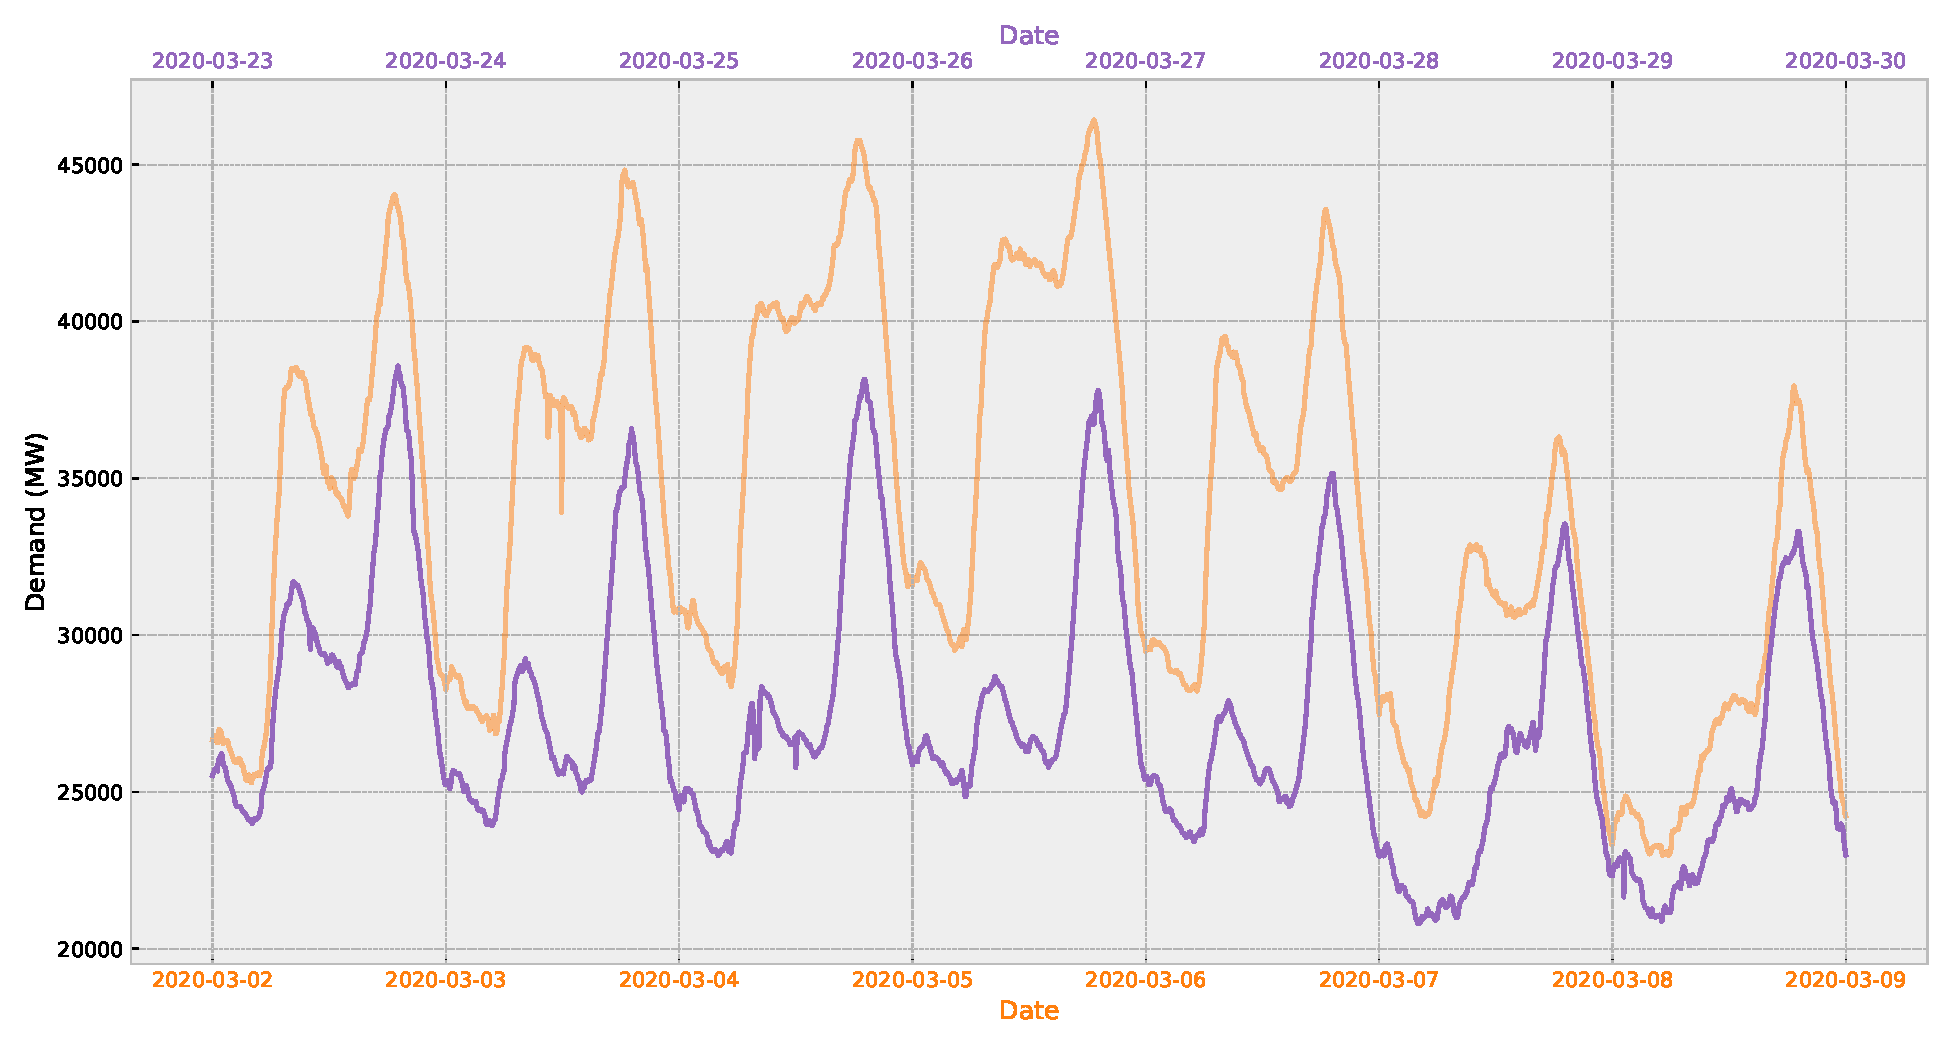
\includegraphics[width=15 cm]{Graphics/Demand_profiles.pdf}
\caption{Aggregated system demand before and after the COVID-19 actions}\label{fig:demand_profiles}
\end{figure}  

Figure \ref{fig:Demand_hist}, shows the demand histogram shifted to the left, indicating lower loads. The lighter colour (i.e.mostly yellow) peak for the post-action demand show that the range of most occurring demand values is now narrower, meaning there is less variation. Otherwise, the pre-action demand shows a more disperse and even occurrence profile which looks slightly bi-modal. The bi-modality, meaning that two occurrence centres exist, can be related to work-hours and non work-hours. While during non-work hours the profile is levelled on the base load and work-hours show another load centre. In conclusion, the effects taken after the COVID-19 actions denoting a higher occurrence of lower demands which results in a smoother load profile.

%For creating a predictive model, perhaps this would be divided into two groups

\begin{figure}[H] 
\centering
\hspace{-25pt}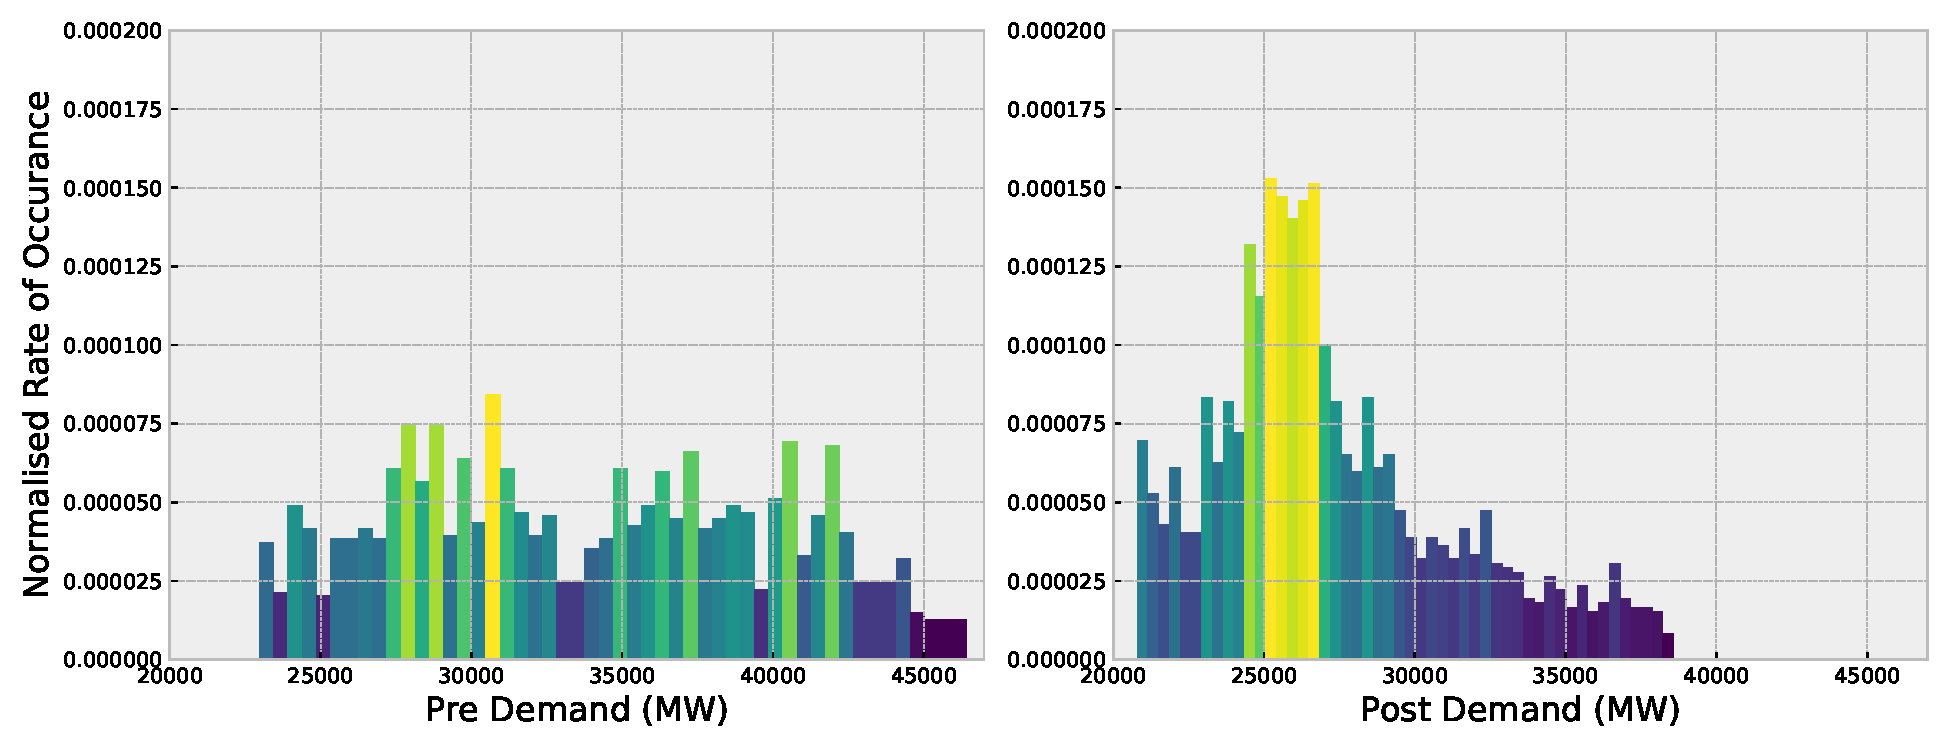
\includegraphics[width=16.5 cm]{Graphics/Demand_hist_coloured_sidebyside.pdf}
\caption{Comparison of pre- and post-COVID-19 demand histograms with normalised occurrences. The range of colours from yellow to dark blue correspond to the highest and lowest values.}\label{fig:Demand_hist}
\end{figure}  

Load duration curves are used in power engineering to visualise the base and peak load and how often certain power demands occur between them. In Figure \ref{fig:load_duration}, the load duration curves are plotted for the pre and post action case. The visual changes are determined in Table \ref{table:load-duration}. While the base load only drops slightly by -9.50\%, the peak load drops much further by -20.31\%. However, the mean load drops the most, namely by -24.08\%, showing that the most load reductions happening between peak and baseload and smoothing the load profile.  %visualise the relationship between sorted demand (i.e. ranked descending) and time. %It is used to analyse the variation in energy (i.e in Figure \ref{fig:load_duration}, the area of the graph gives the energy used in MWh) and choose baseload and peak load power for generators. 

\begin{figure}[b]
\centering
\hspace{-25pt}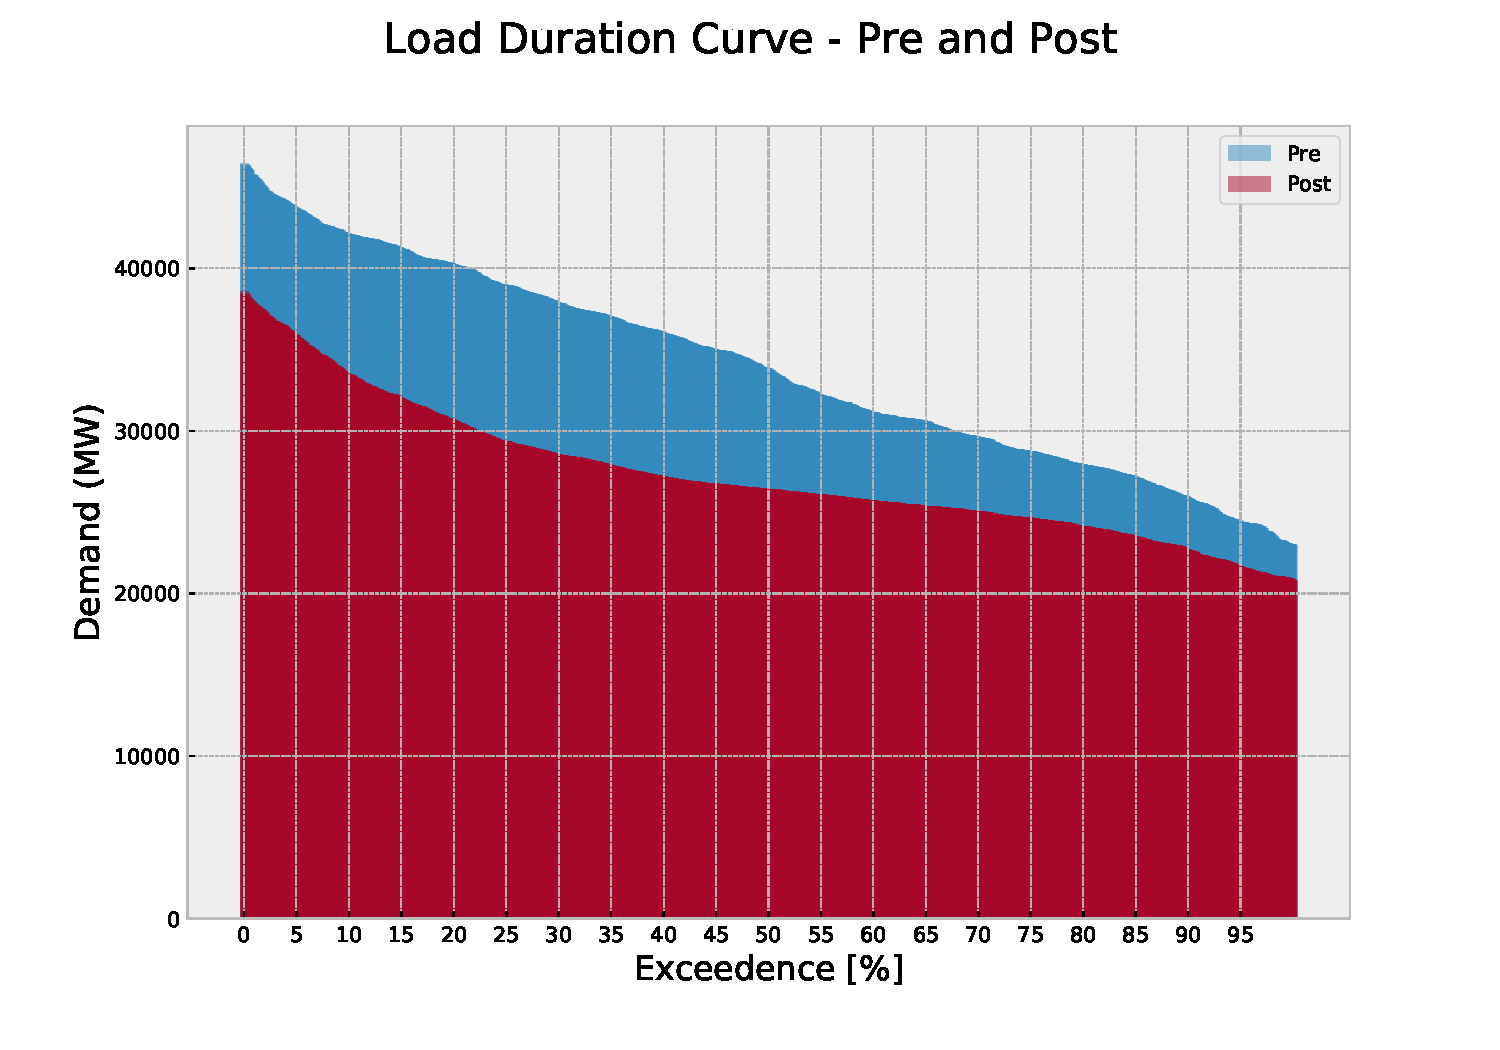
\includegraphics[width=9 cm]{Graphics/Load_duration_curve.pdf}
\caption{Load duration curve for pre- and post-COVID-19 actions.}\label{fig:load_duration}
\end{figure}  

\begin{table}[H]
\caption{Changes in demand profile using the data from the load duration curves. }
\centering
%% \tablesize{} %% You can specify the fontsize here, e.g., \tablesize{\footnotesize}. If commented out \small will be used.
\begin{tabular}{ccccccc}
\toprule
\textbf{Profile} & \textbf{Peak Load (MW)}	& \textbf{\%} & \textbf{ Mean Load (MW)}	& \textbf{\%}	& \textbf{ Base Load (MW)}	& \textbf{\%}\\
\midrule
Pre	& 46425 & & 33868 & & 22982 &  \\
Post & 38585 & \textcolor{red}{-20.31\%} & 27294 & \textcolor{red}{-24.08\%} & 20795 & \textcolor{red}{-9.5\%} \\

\bottomrule
\end{tabular}
\label{table:load-duration}
\end{table}

%\textcolor{purple}{
%\textbf{Quick Results so far}
%\begin{itemize}
%    \item 20.31\% decrease in Peak Demand
%    \item 24.08\% decrease in Mean Demand
%    \item Only 10\% decrease in Base Load
%    \item 1 hour shift in "morning peak" - 9 am to 8 am and "evening peak" - 6 pm to 7 pm
%    \item Steeper climb to the "evening peak" - used to be 7500 MW increase over 4 hours, now it is 9500 MW increase in 5 hours.
%    \item Overall decrease in Peak-to-Mean ratio -except  7, 8, 9 am. However, it seems to follow the same morning trend as the pre data which had its max PtM value at 6 am at 0.18. This peak is delayed to 8 am and decreased by 1. 
%    \item Speculation: People wake up later, eat dinner earlier :)
%    \item Standard deviation is smaller by a third of its original value (i.e. 6085). Presumably, this could explain the better performance of forecasting algorithms.
%\end{itemize}
%}

%Figure \ref{fig: PtM_Ratio_Demand_comp} and \ref{fig: PtM_Ratio_Demand} uses the peak-to-mean ratio ($max/mean$) in order to quantify the variation in the consumption profile. 


%\begin{figure}[H]
%\centering
%\hspace{-25pt}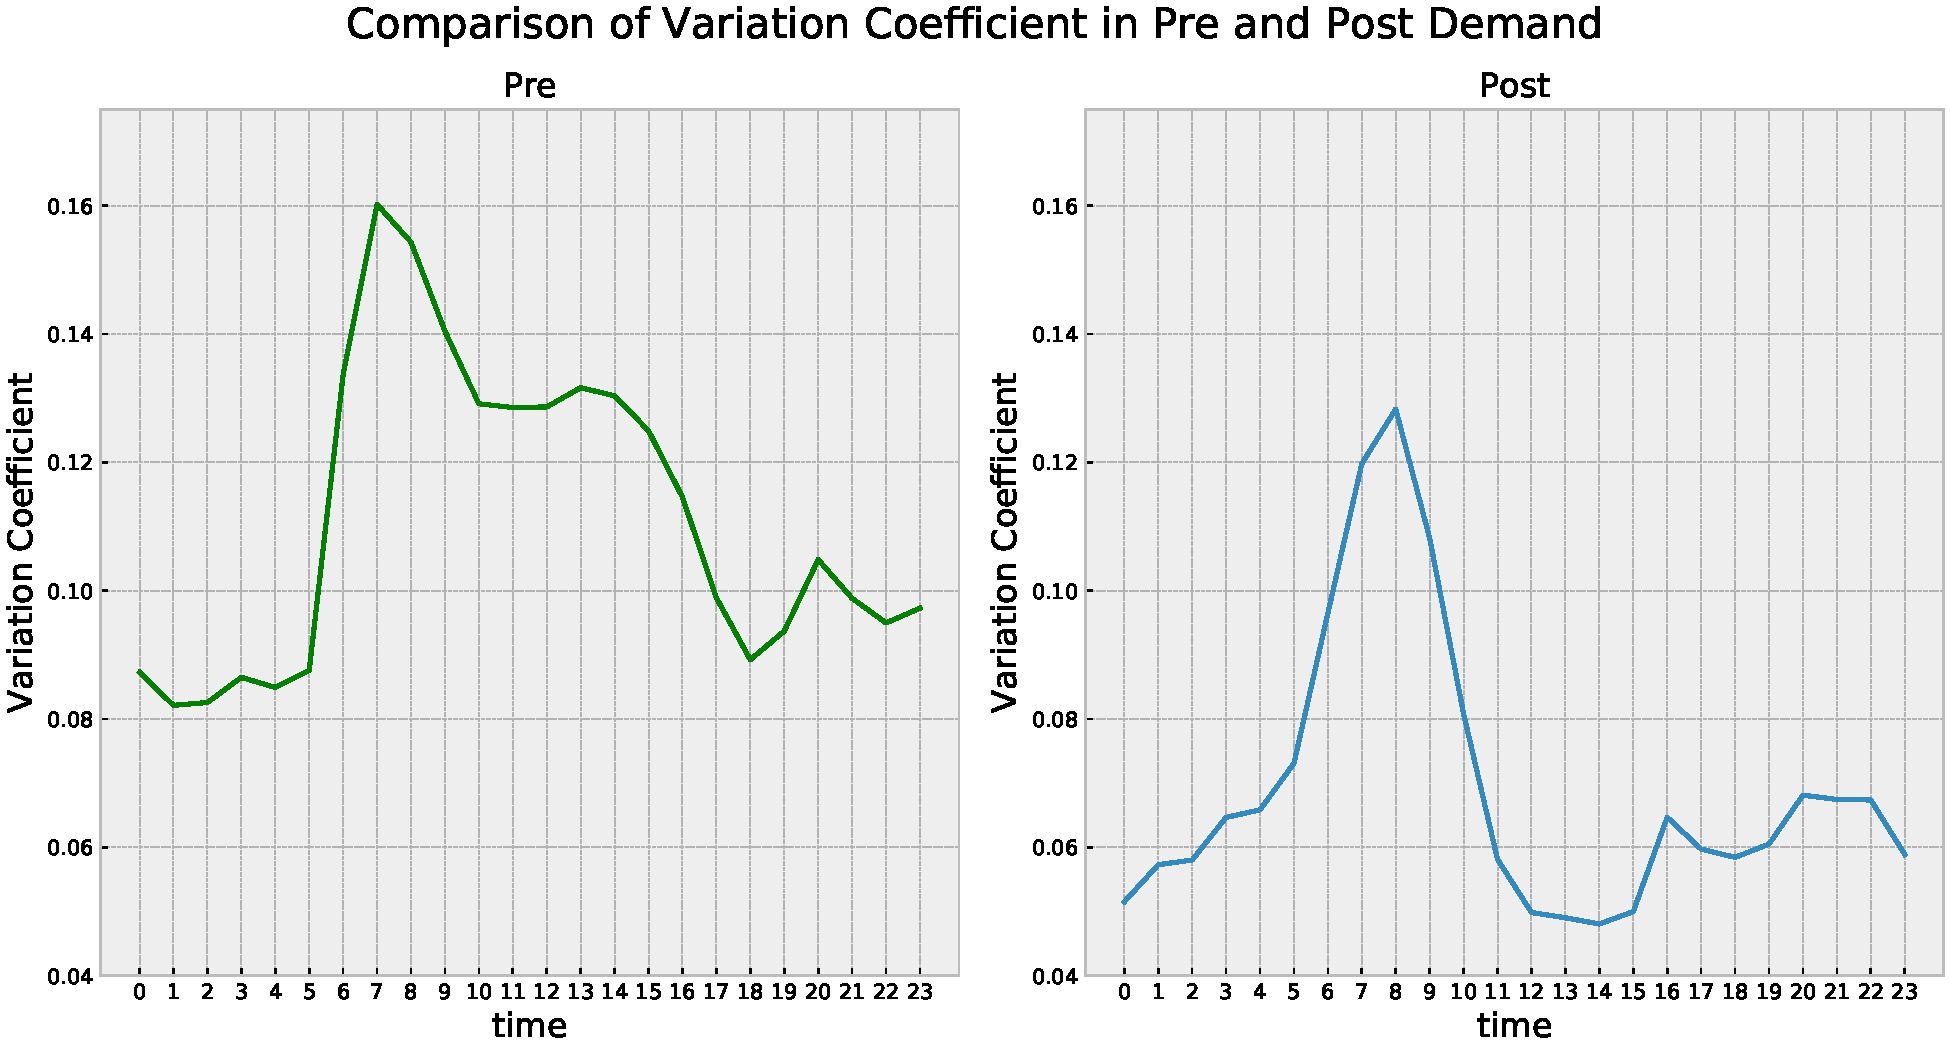
\includegraphics[width=15 cm]{Graphics/VarCoeff_comp.pdf}
%\caption{Comparison of peak-to-mean ratio to visualise the variation in system demand.}\label{fig: PtM_Ratio_Demand_comp}
%\end{figure}  

%\begin{figure}[H]
%\centering
%\hspace{-25pt}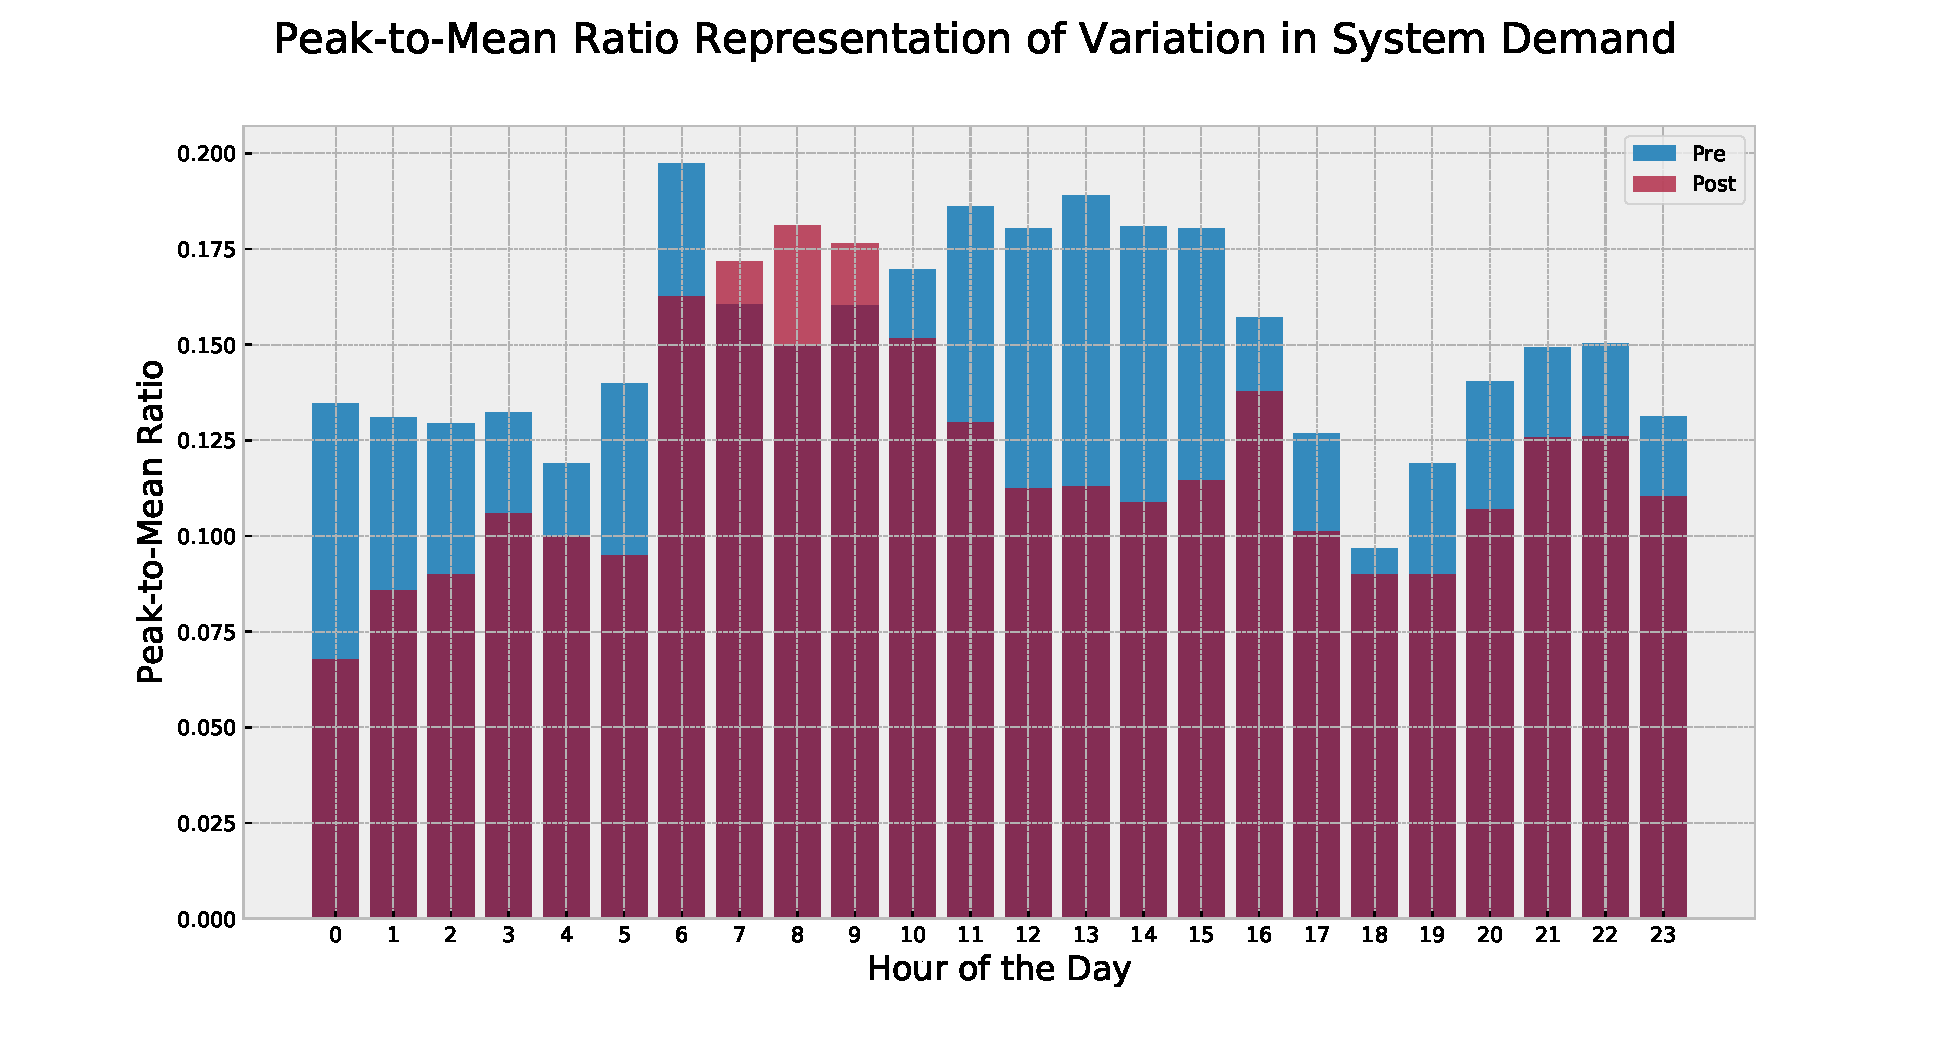
\includegraphics[width=7 %cm]{Graphics/PtM_ratio_Demand.pdf}
%\caption{Overlaying the peak-to-mean ratios to compare the variation in system demand.}\label{fig: PtM_Ratio_Demand}
%\end{figure}


%\begin{figure}[H]
%\centering
%\hspace{-25pt}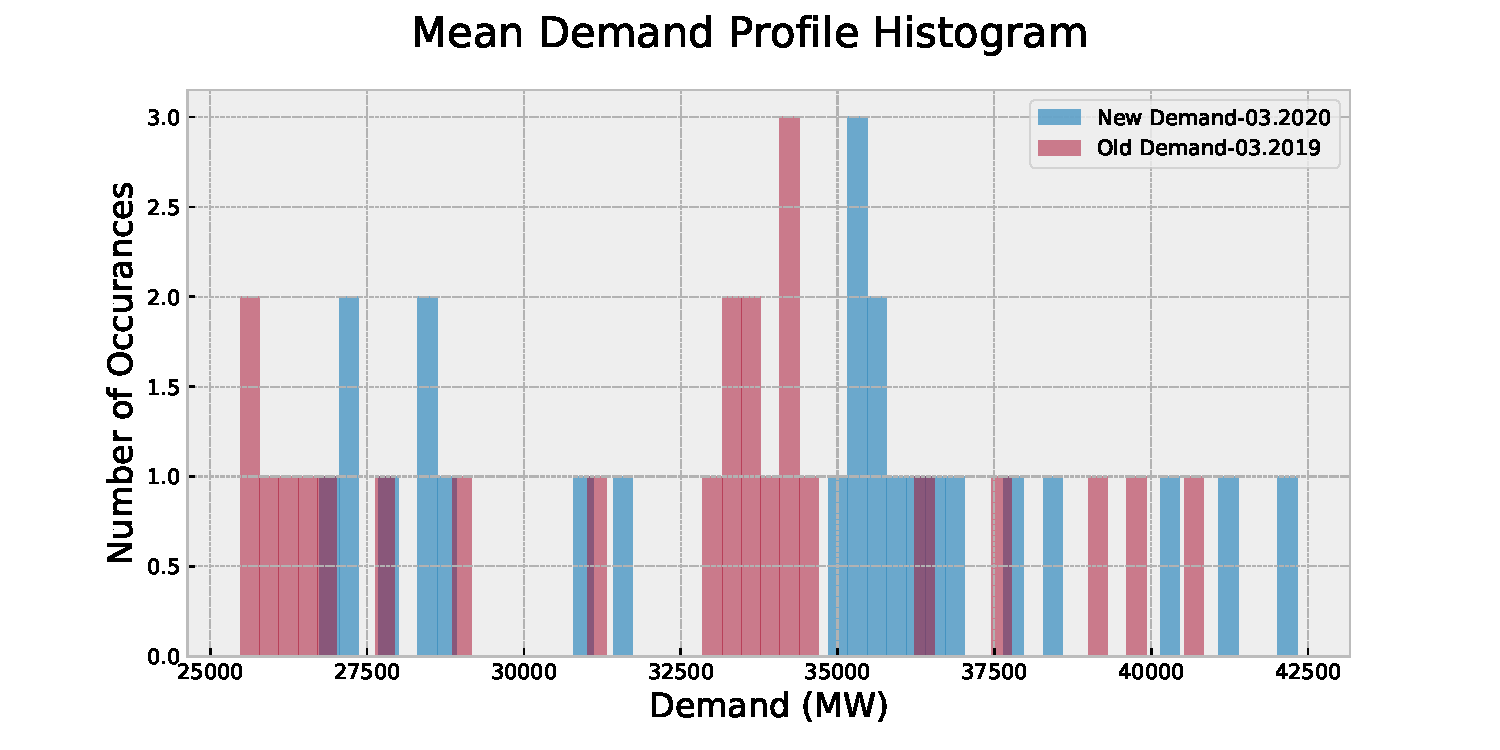
\includegraphics[width=16.5 cm]{Graphics/Mean_Demand_Profile_hist.pdf}
%\caption{}
%\end{figure}  

%\textcolor{blue}{
%\begin{itemize}
%    \item Coefficient of variation (=standard deviation/mean)
%    \item Peak-to-mean ratio
%    \item Inter-quartile range
%\end{itemize}}




% \begin{figure}[H]
% \centering
% \hspace{-25pt}\includegraphics[width=15 cm]{Graphics/CORR1.pdf}
% \caption{Correlation of Demand and Generation by Fuel type}\label{fig:demand_profiles}
% \end{figure}  


% \begin{table}[H]
% \caption{Comparison of statistical descriptors to quantify the changes in the demand pre- and post-COVID-19 mitigation actions. }
% \centering
% %% \tablesize{} %% You can specify the fontsize here, e.g., \tablesize{\footnotesize}. If commented out \small will be used.
% \begin{tabular}{cccc}
% \toprule
% \textbf{Demand Data} & \textbf{Coefficient of variation}	& \textbf{Peak-to-mean ratio}	& \textbf{Inter-quartile range}\\
% \midrule
% March 2019		& data			& data         &data\\
% March 2020		& data			& data         &data\\
% Other years also&data          &data           &data\\
% \bottomrule
% \end{tabular}
% \end{table}

%%%%%%%%%%%%%%%%%%%%%%%%%%%%%%%%%%%%%%%%%%%

\subsection{Generation Portfolio}\label{sec:Generation portfolio}
The change in the demand profile leads to change in the generation portfolio. In particular, the lower demand enlarge the shares of variable renewable energy (VRE), namely wind and solar, which further impacts the conventional generation portfolio in the power system. 

\subsubsection{The VRE share growths}
The hypothesis for a increased VRE share originates from the causality principles in electricity markets and supported by a simple example. 
First, most generators are scheduled in European electricity markets in merit-order, which means the least marginal cost generators are supplying the power demand. The causality is VRE generators have marginal costs close to zero, which leads to the effect that VRE's are mostly scheduled before any other generation technology in electricity markets \cite{Winkler2016ImpactMatter}. As the VRE infrastructure already exist, preferred in scheduling and the VRE generation is not restricted by the COVID situation, it can be justifiably hypothesised that on average a lower demand increase the shares of VRE. 

Second, to support the hypothesis it must be realised, the VRE share depends beside the total generation or load, on the weather conditions which impact the VRE output in every point in time. Changing weather conditions make it hard to compare any weeks with non-complex methods. Therefore, Figure \ref{fig:generation_effects} illustrate a simplified qualitative example which keeps the VRE generated output stable, representing constant solar and wind conditions in a i) high demand case and ii) low demand case. The high and low demand cases are chosen in such a way that the values are easy to understand and representing the observed changes of the COVID situation in GB. For instance, the in section \ref{section: Effect on demand profile} recognised average changes of the demand where approximately 25 \%, while the average VRE share in March was roughly 25 \% based on ENTSO-E data \cite{ENTSO-E2020ENTSO-EPlatform}. The total demand and generation are set equal in each case, hence, representing a stable power system. As result of the previous hypothesis and Figure \ref{fig:generation_effects}, the average demand reduction lead to higher VRE shares. The results from Figure \ref{fig:generation_effects}, further indicate that the VRE share could increases in the range of 5-10 \% in the GB system due to the new demand profile.


\begin{figure}[H]
\centering
\hspace{-25pt}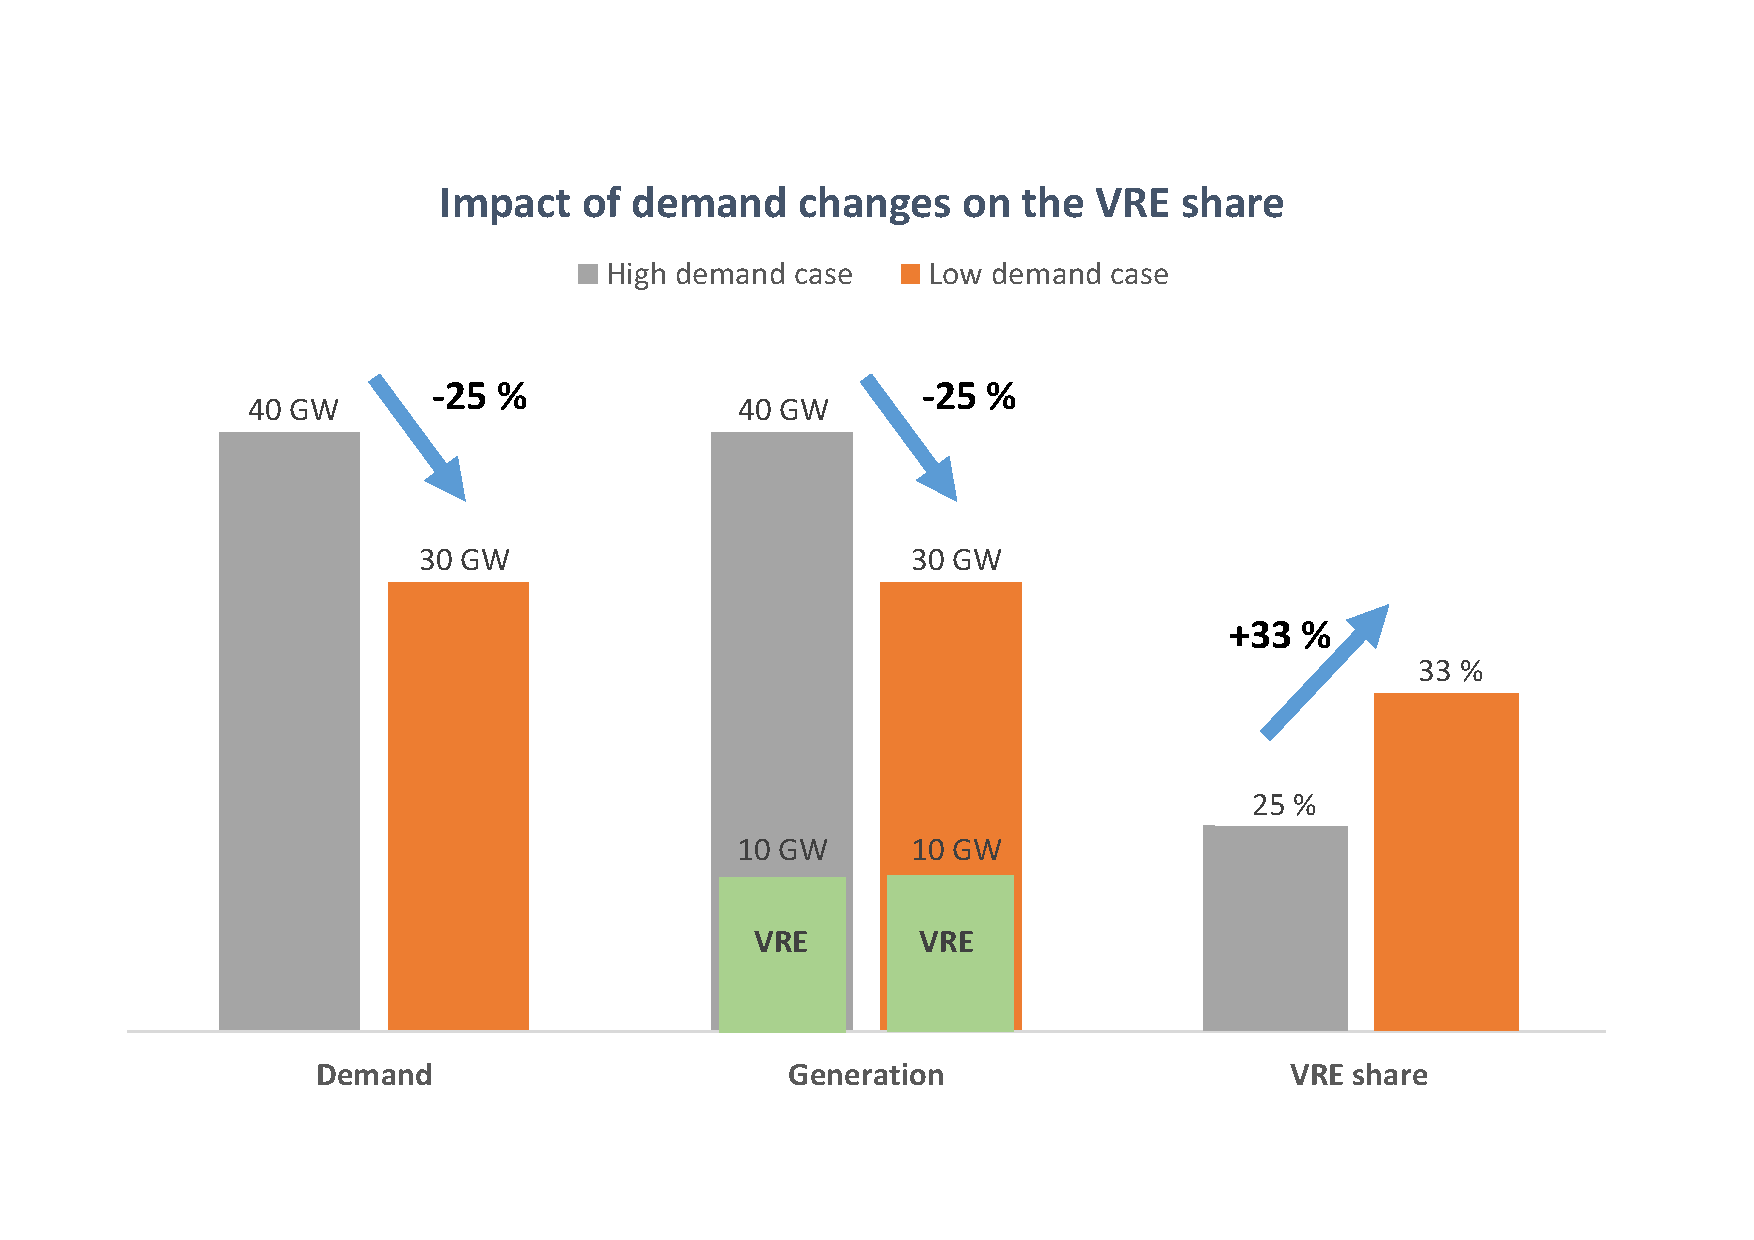
\includegraphics[trim={0cm 2cm 0cm 2cm},clip,width=1\textwidth]{Graphics/Illustrative-VRE-share-increase.pdf}
\caption{Qualitative example of the impact of demand changes on the VRE share. Share of VRE share, and ratio demand changes equal roughly the UK case, check \protect\cite{ENTSO-E2020ENTSO-EPlatform} and section \protect\ref{section: Effect on demand profile}, respectively.}
\label{fig:generation_effects}
\end{figure} 

\subsubsection{Impact on the conventional generation portfolio}

The conventional generation portfolio, including all generation assets with marginal cost above solar and wind technologies, are expected to decrease in operation time compared to the situation without lock-down. The reason is beside the lower total demand, the higher share of VRE assets. The higher share of VRE assets at low demand cause additionally a need for more flexibility in the power system - such as provided from gas plants \cite{Hirth2014TheVariability}. If inflexible plants are not reducing their generation the more often negative prices will occur \cite{IEA2016Re-poweringSystems.,Cochran2013MarketSystems}.

%Therefore, the question arises how to compare the VRE share for two weeks with different VRE potential. The answer is factorising both weeks to each other.

%In Figure \ref{fig:generation_effects}, a pre-COVID week was factorised with a post-COVID week for the absolute VRE generation and the total VRE share in the power system. When looking on the lock-down day, the VRE generation increased from pre- to post COVID week by 126 \%, while the total VRE share increased by 169 \%, which result in a difference of 43 \%. On typical days the percentage difference might vary in small ranges as new VRE capacity might be added to the power system or due to load variations. Otherwise, the lock-down lead to a drastic lower demand profile, which increased the percentage difference over-proportional. One could question why in Figure \ref{fig:generation_effects} the percentage difference on Sunday is low. One reason is that on a typical Sunday most businesses are closed and therefore the load profile doesn't vary too much from COVID load profile. In conclusion, the observed data can interpreted as evidence that the lower demand leads to a higher share of VRE in the power system. 

%\begin{figure}[H]
%\centering
%\hspace{-25pt}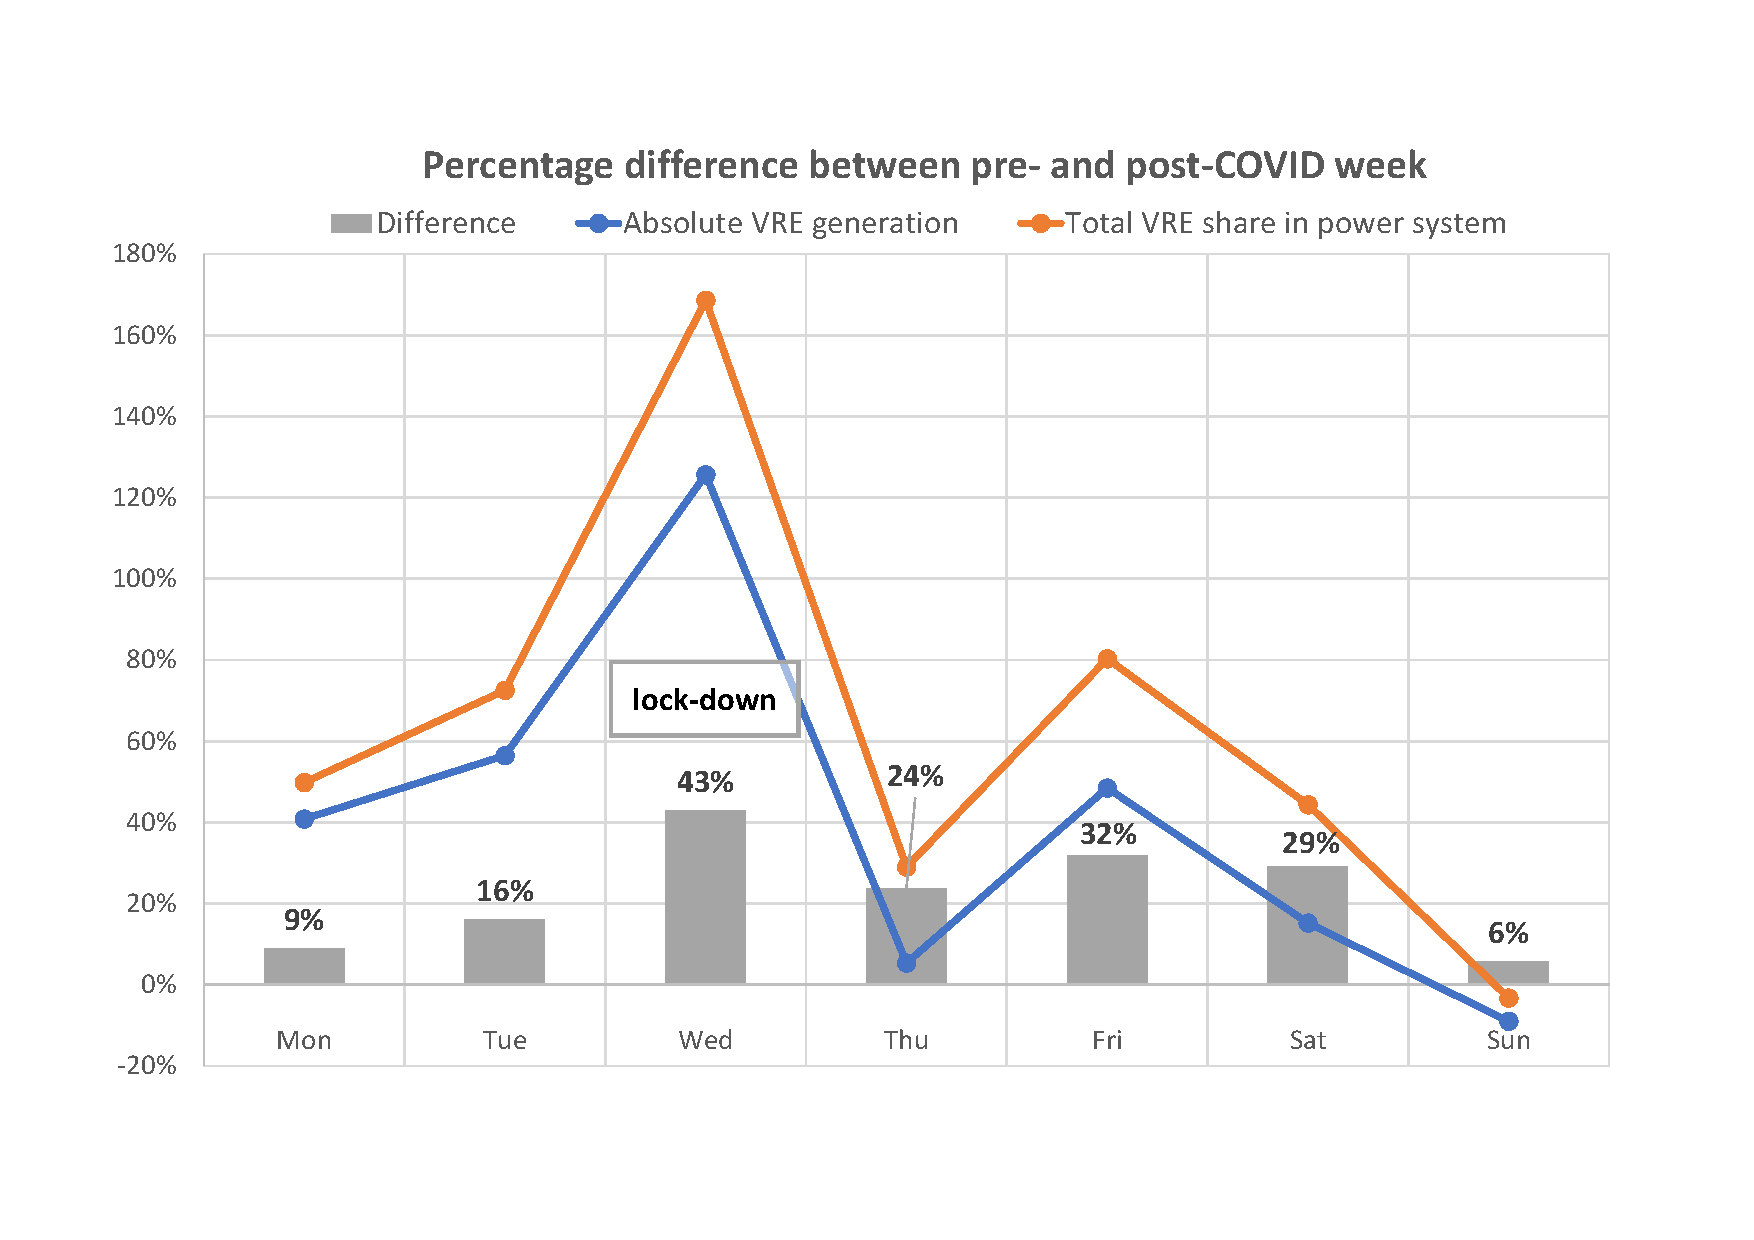
\includegraphics[trim={0cm 2.5cm 0cm 2.5cm},clip,width=1\textwidth]{Graphics/Weather-independent-VRE-Share-increase.pdf}
%\caption{Percentage difference for i) VRE generation and ii) VRE share in the power system in the pre- and post-COVID week, 02-09 March and 22-28 March, respectively. While zero percentage represent the pre-COVID daily baseline, the coloured points represent a grow or decrease factor for the post-COVID week. Data extracted from ENTSO-E transparency platform \protect\cite{ENTSO-E2020ENTSO-EPlatform}.}
%\label{fig:generation_effects}
%\end{figure} 

%%%%%%%%%%%%%%%%%%%%%%%%%%%%%%%%%%%%%%%%%%%%%%%%%%%%%%%%%%%%%%%%%%%%%%%%%%%%%%%%%%%%%%
\subsection{Forecasting and Grid Stability}
\subsubsection{Load Forecast Error}\label{DemandForecastError}
In this chapter, the short-term load forecast effects due to COVID-19 are analysed in the GB power system. In contrast to mid- and long-term load forecast, which make predictions above months and years, respectively, the short-term load forecast make predictions for hours up to weeks before the settlement period \cite{SahayDayNetwork,Khuntia2016ForecastingReview}. Short-term load forecasting plays an important role in scheduling the power plants efficiently in electricity market, as economic dispatch and unit commitment requires load forecasts \cite{He2020Day-aheadForest}. As result, improving the forecast accuracy lead to a more reliable and affordable power system \cite{SahayDayNetwork}. 

Two different short-term load forecast were analysed in this study, the Day-Ahead total load forecast (DAF) and the transmission system final load forecast (TSF). The DAF and TSF differ in methodology and forecast length. First, in regard to the methodology, the DAF represent a forecast for the total load in the power system, which equals the sum of generated power on both, TSO and DSO networks \cite{ENTSO-E2020ENTSO-EPlatform}. Otherwise TSF, represents a load forecast which equals the sum of generation which can be seen from TSO network only - this include, though, generation from pump storage and embedded large power plant on DSO network level \cite{NationalGrid2020THE40}. The TSF can be therefore interpreted as the "net demand" which the electricity market participants must supply while the DAF represents the real experienced total load in the power system. Second, the forecast length, which describes the time from forecast publication until actual operation time, varies in the collected data for DAF and TSF, see Figure \ref{fig:forecast_length_explanation}. The DAF is published only once a day and predict for the next day the average demand in each settlement period, hence, the forecast length vary from 12-36 hours \cite{ENTSO-E2020ENTSO-EPlatform}. Similarly, the TSF publishes a Day-Ahead forecast, however each settlement period is updated in the TSF data until it reaches the final TSF which predicts the next average demand in the settlement period 1:15 h ahead \cite{ELEXON2020ELEXONBMRS}.

\begin{figure}[H]
\centering
\hspace{-25pt}
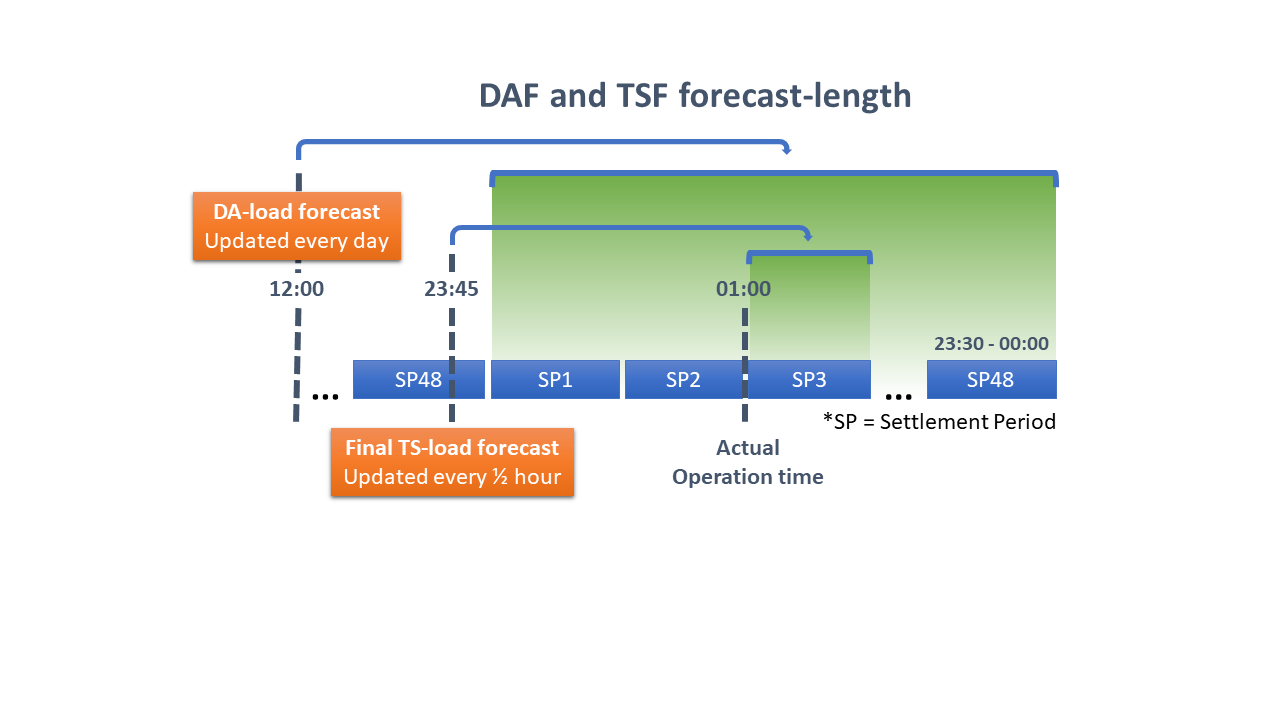
\includegraphics[trim={2cm 5cm 2 2cm},clip,width=1.1\textwidth]{Graphics/Forecast explanation.png}
\caption{Illustrative forecast lengths for the total Day-Ahead load forecast (DAF) and the final transmission system load forecast (TSF).}
\label{fig:forecast_length_explanation}
\end{figure} 

Interestingly, the DAF and TSF forecast errors reveal different characteristics due to the lock-down. The DAF forecast improves while the TSF forecast doesn't show clear changes, see Figure \ref{fig:DAFandTSFerror}. The forecast error is thereby evaluated by one of the most common performance indicators - the mean absolute percentage error (MAPE) \cite{SahayDayNetwork, He2020Day-aheadForest}. The MAPE is good and simple forecast performance indicator when looking into historical data, however, for prediction model selection and estimation it is biased \cite{Tofallis2015AEstimation}. Nevertheless, in this study only historical data is analysed which make the MAPE suitable. The MAPE is defined as the summed forecast errors, whereby each forecast error is based on the actual load:

\[ MAPE(\%) = \frac{1}{N} \sum_{i=1}^N \frac{y_{i,actual} - \hat{y}_{i,forecast}}{y_{i,actual}} \]

In general, the longer the forecast length is for the same time resolution, the higher the forecast error becomes \cite{NationalgridESO2018QuarterlyMarch18}. Therefore the forecast error constitutes on average higher forecast errors for the DAF than for TSF. In regards to the lock-down effects, the higher forecast accuracy for the DAF is especially remarkable when distilling the time frame on the weekdays from Wednesday to Friday - the weekdays where the lock-down occurred. The typical working week differs much more from the lock-down working week, and the weekend is much more similar to the lock-down weekend, hence smoothing the lock-down effects when the full calendar week is averaged. Contrary, the TSF doesn't show clear effects due to the lock-down, which imply that the shorter-length forecast is less effected by the lock-down.

Of course the change of the forecast error cannot be solely retraced to the lock-down, since the forecast error is affected by many circumstances. In \cite{NationalgridESO2018QuarterlyMarch18}, a list of components of forecast errors are given. Nevertheless, in particular, the DAF shows a clear untypical change of magnitude that could indicate that the lock improved the Day-Ahead forecast. A reason could be the smoother, less variable demand profile which was recognised in section \ref{section: Effect on demand profile}. Even though the impact of the TSF change cannot be solely traced back to lock-down due to minimal visible changes, in combination with the imbalance discoveries in section \ref{}, the short-length forecast accuracy decrease evidently.


%\begin{figure}[H]
%\centering
%\hspace{-25pt}
%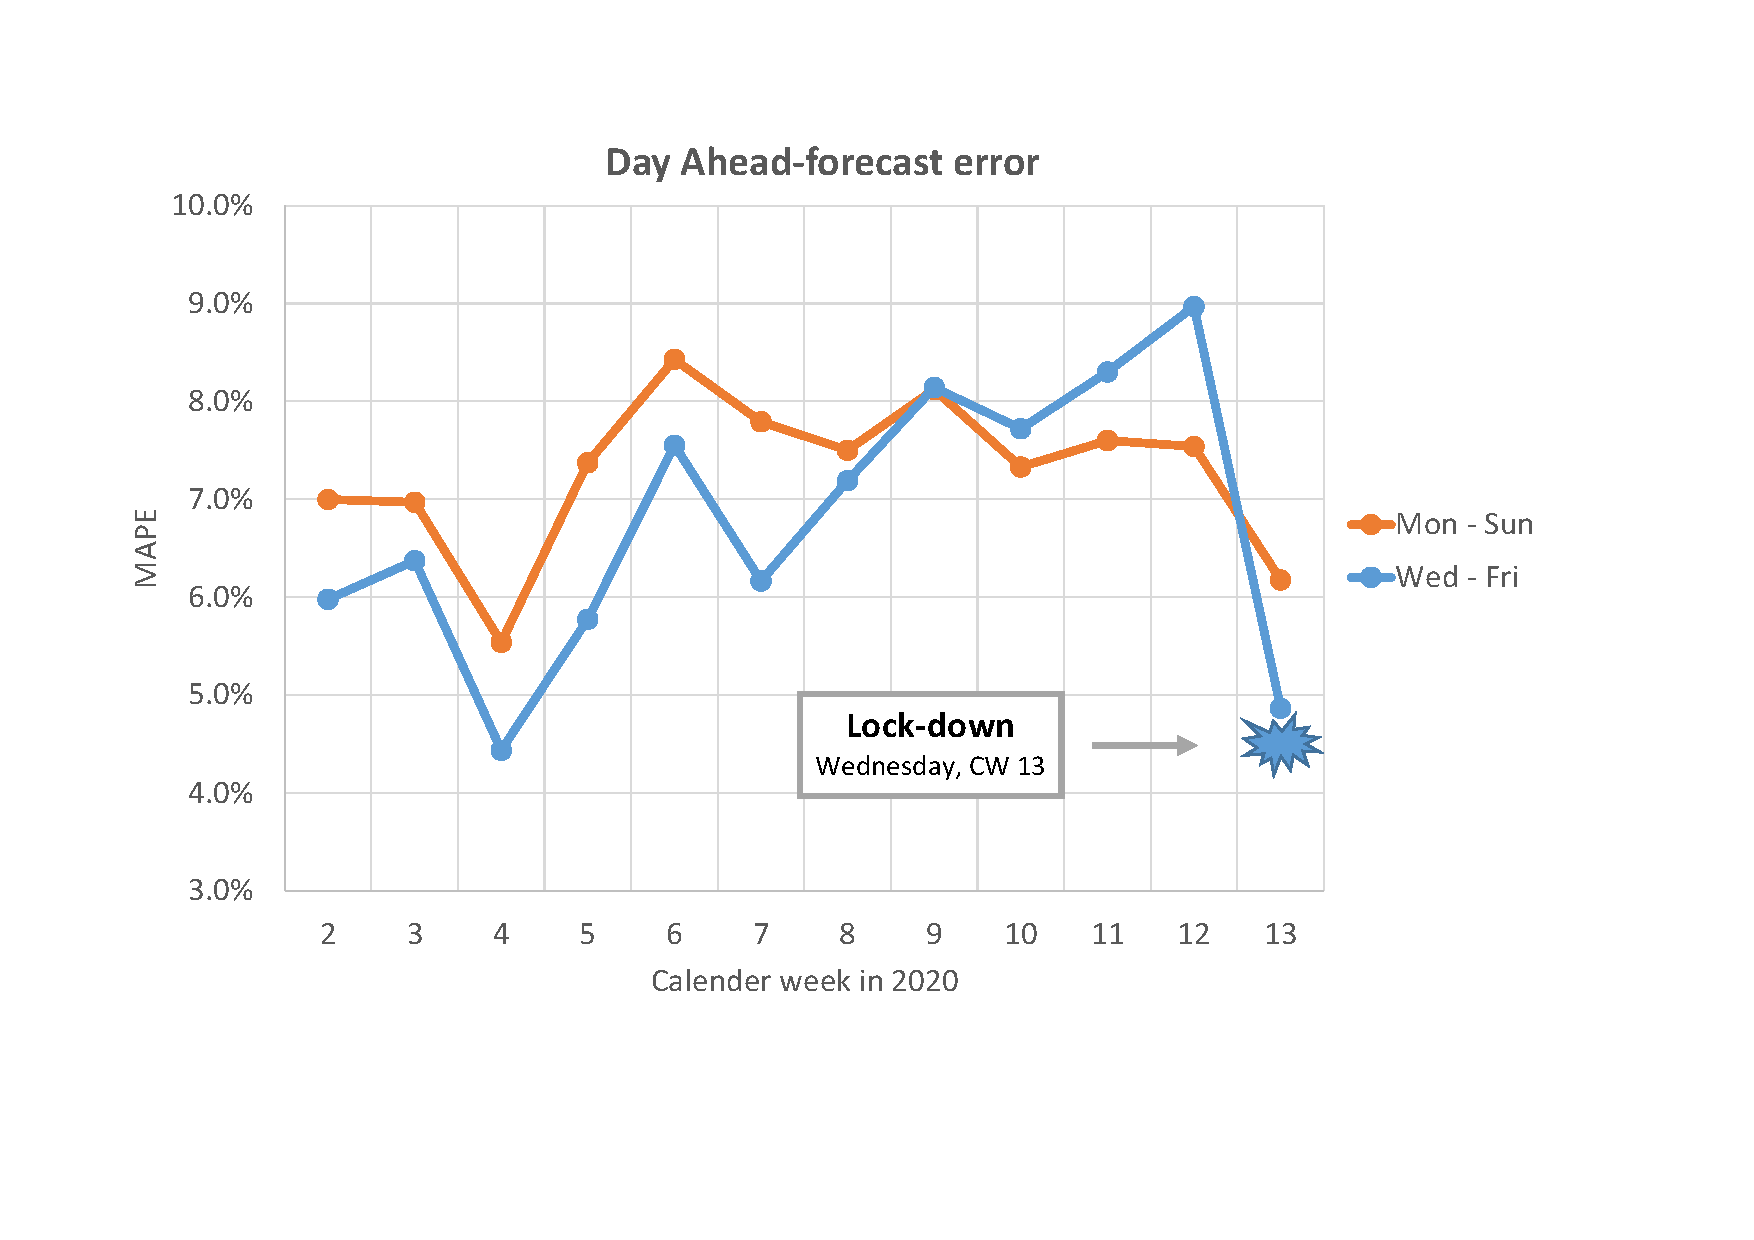
\includegraphics[trim={0cm 3cm 1cm 0.1cm},clip,width=16.5 cm]{Graphics/DAF-error.pdf}
%\caption{Weekly aggregated total Day-Ahead load forecast (DAF) error for the time frame from i) Monday to Sunday and ii) Wednesday to Sunday }
%\label{fig:DAF_forecast_error}
%\end{figure} 

%\begin{figure}[H]
%\centering
%\hspace{-25pt}
%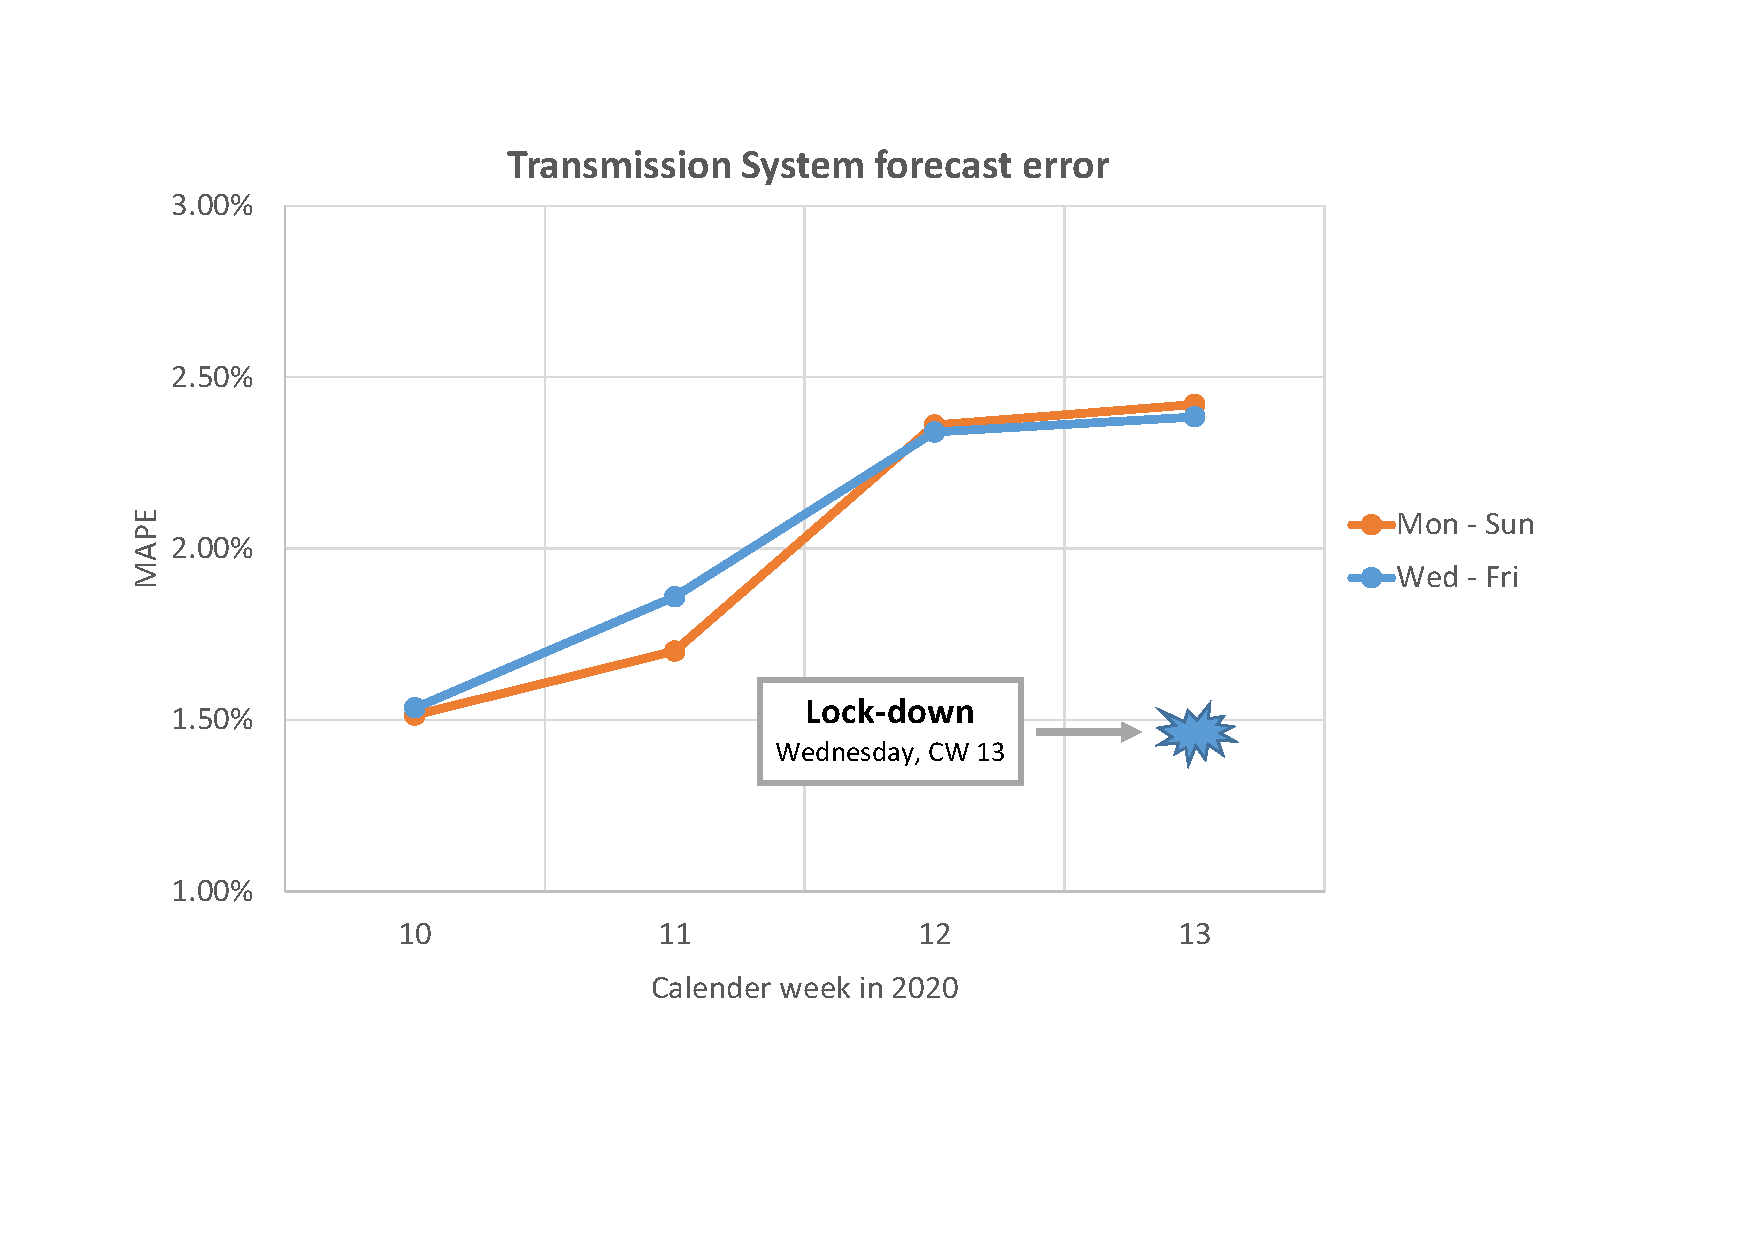
\includegraphics[trim={0cm 3cm 1cm 0.1cm},clip,width=16.5 cm]{Graphics/TSF-error.pdf}
%\caption{Weekly aggregated final transmission system load forecast (TSF) error for the time frame from i) Monday to Sunday and ii) Wednesday to Sunday }
%\label{fig:TSF_forecast_error}
%\end{figure} 


\begin{figure}[!tbp]
  \centering
  \subfloat[DAF error.]{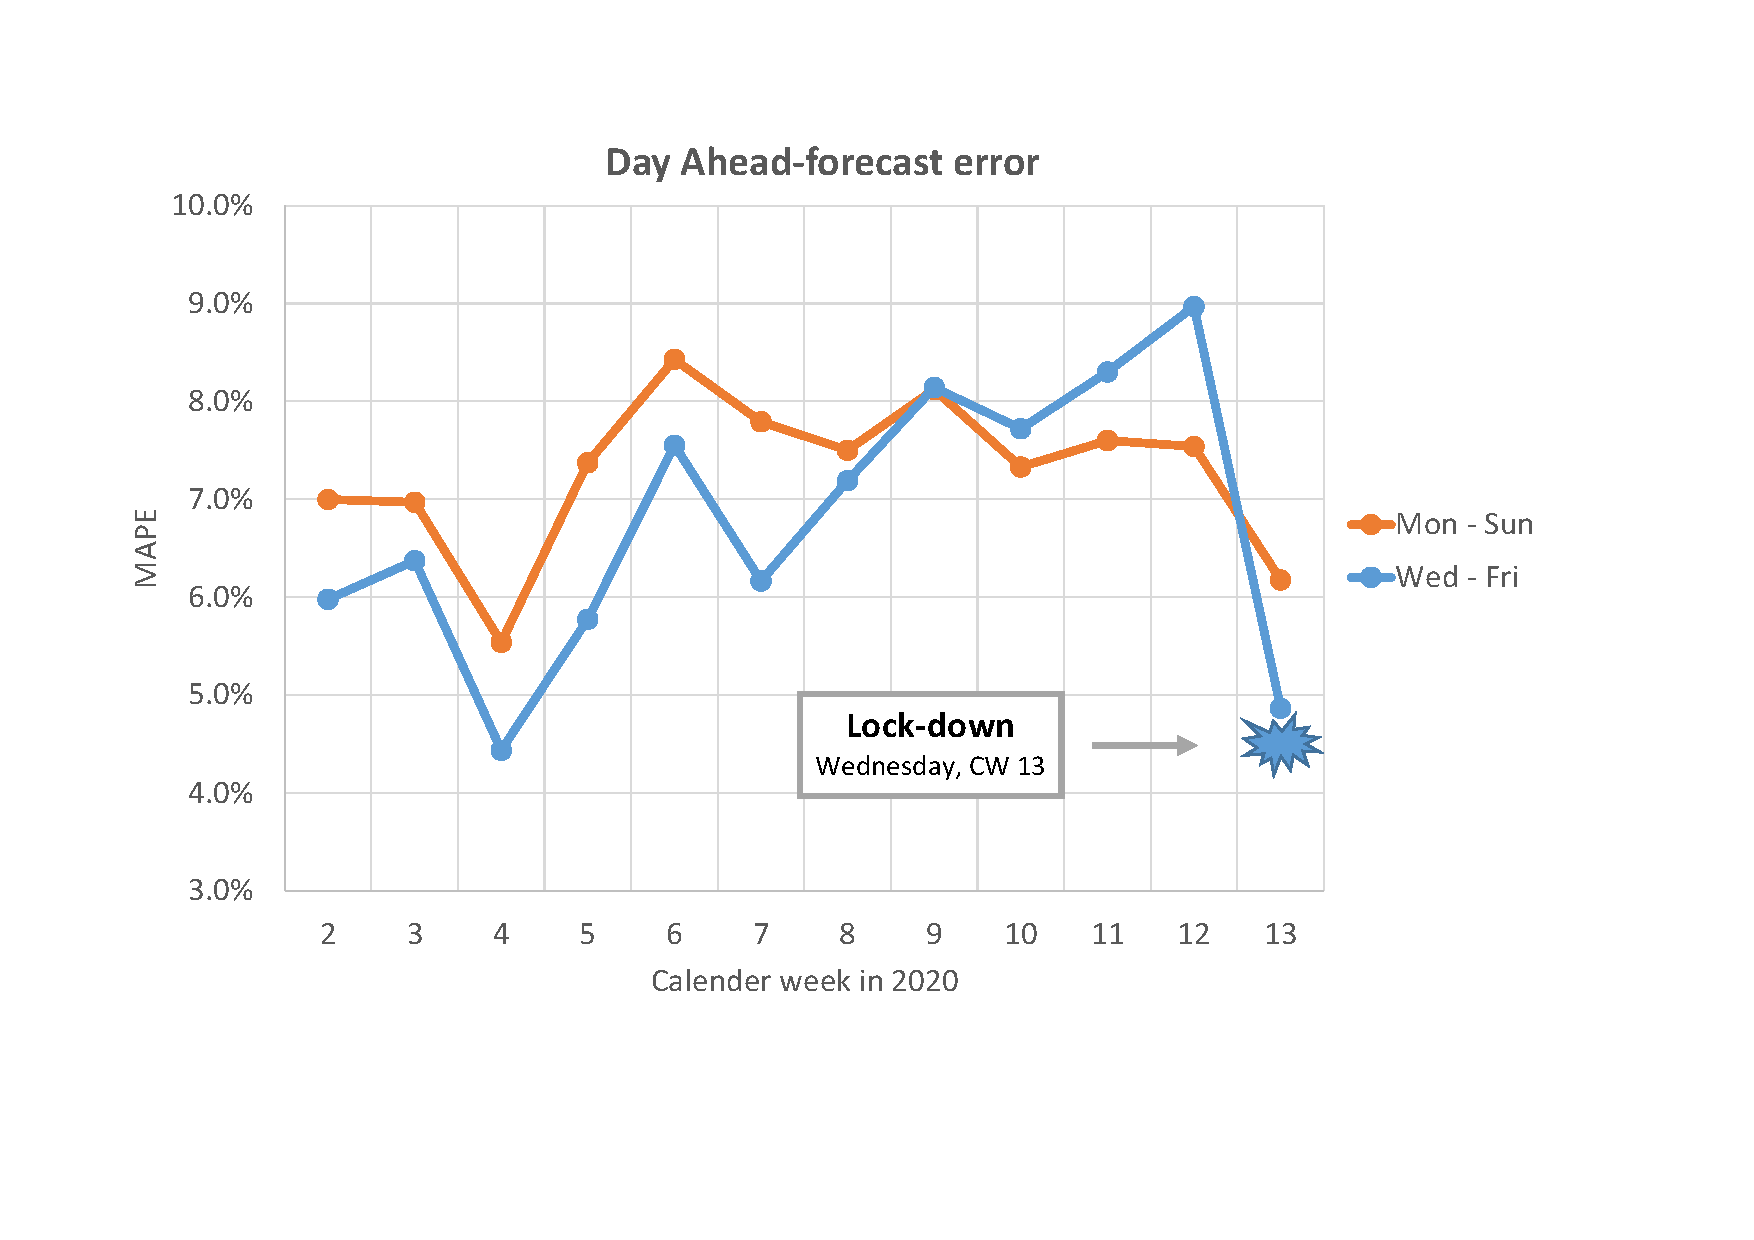
\includegraphics[trim={2cm 3cm 7cm 2cm},clip,width=0.45\textwidth]{Graphics/DAF-error.pdf}\label{fig:DAFerror}}
  \hfill
  \subfloat[TSF error.]{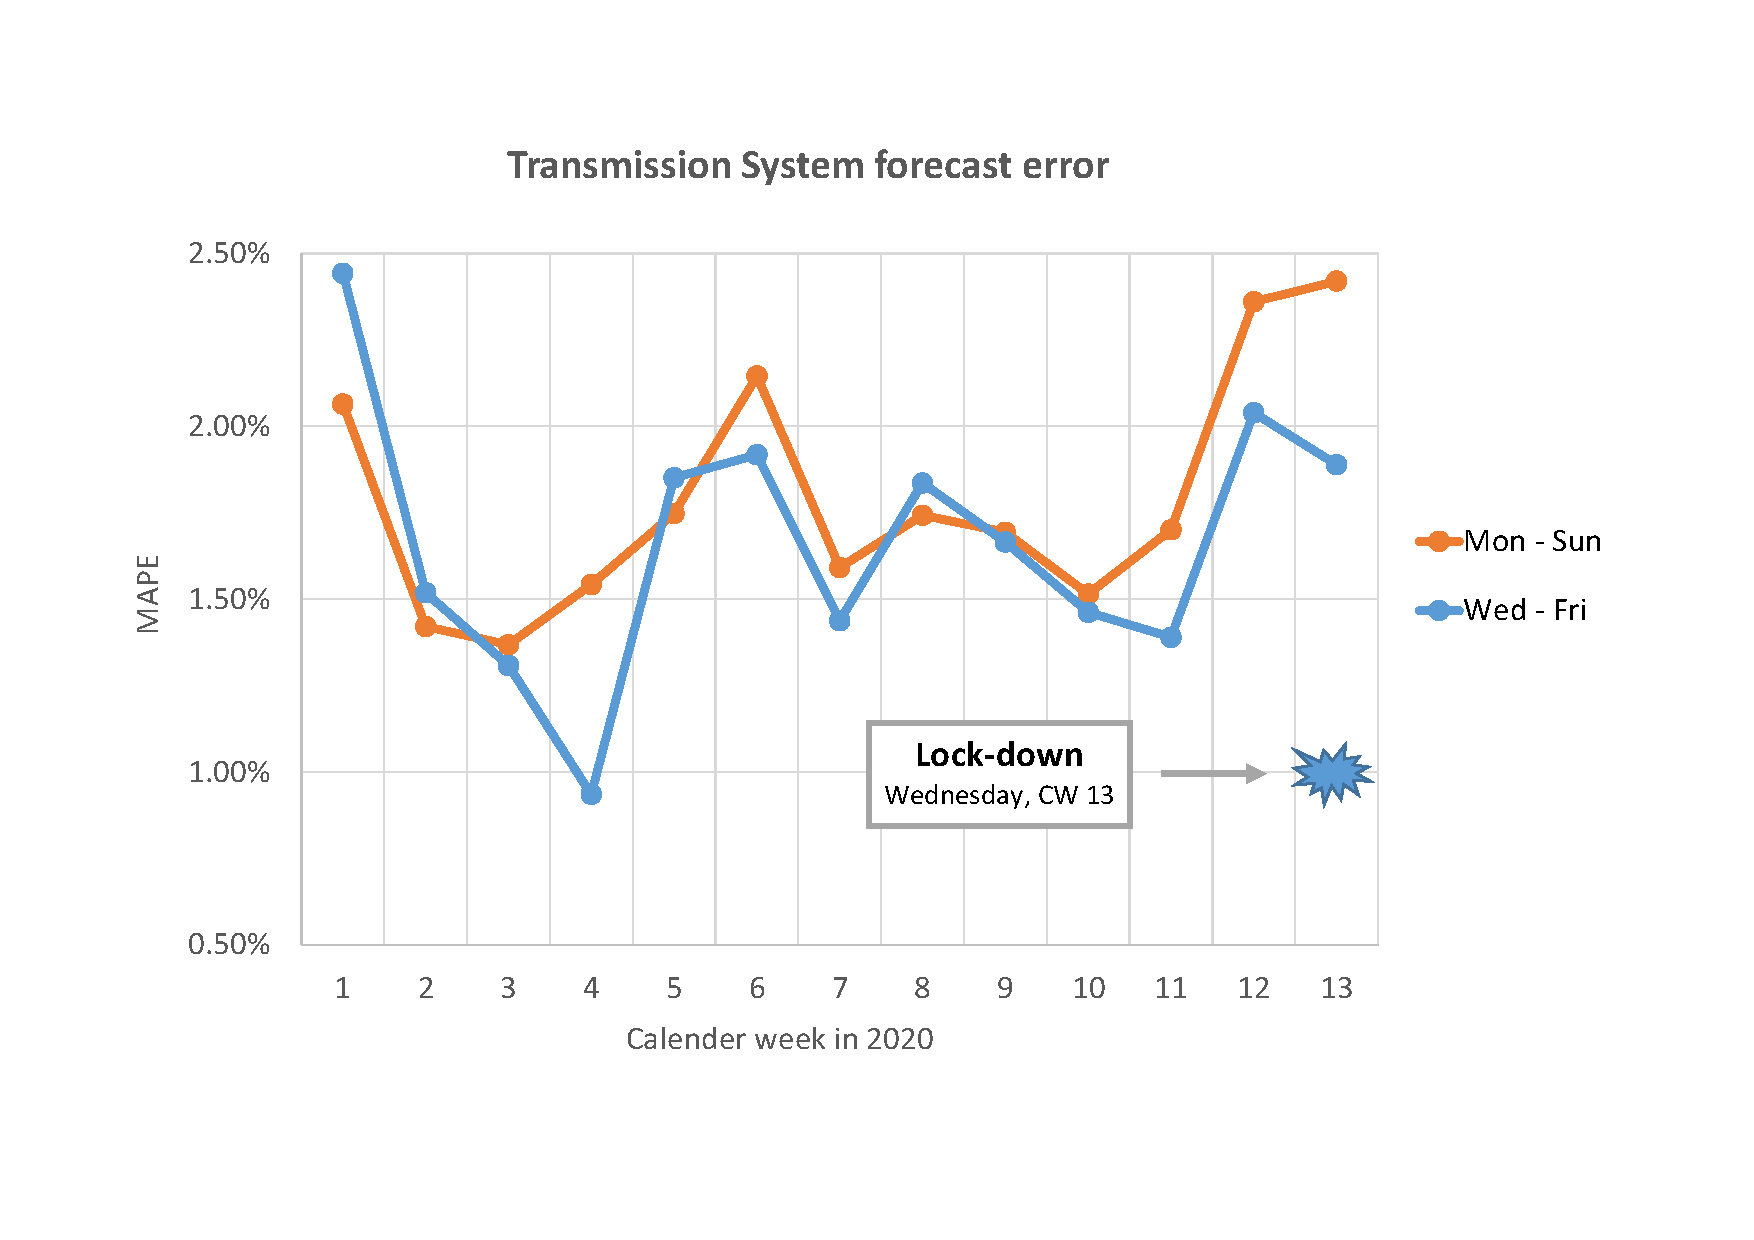
\includegraphics[trim={2cm 2cm 2.5cm 2cm},clip,width=0.53\textwidth]{Graphics/TSF-error-2020.pdf}
  \label{fig:TSFerror}}
  \caption{Weekly aggregated total Day-Ahead load forecast (DAF) and final transmission system load forecast (TSF) error, for the time frame from i) Monday to Sunday and ii) Wednesday to Friday. Note: The Wednesday to Friday frame was used to show the impact of the COVID-lockdown from the workday perspective.}
  \label{fig:DAFandTSFerror}
\end{figure}

%MAX: It seems I don´t have access to real DH data from ELEXON. Therefore, I take the DH data from ENTSO-E for the DH-forecast (long-term) and the ELEXON TSDF for short term forecast - 1h15min before SP.
%Max: It was recognized that both demand data are calculated with a different methodology. (ENTSO-E demand includes effect of all small and large embedded generation unit i.e. household PV or CHP &&& is adding it to the "demand"... Elexon NETSD data however doesn't take into account  net metering, which means that the net demand is smaller for Elexon as home PV is supplying some of the demand..). It of course complicate the comparison between both forecast, however, the general trend of better DH-forecast and worse short-term forecast is valid/interesting even if a "german-apple" is compared with a more delicious "scottish-one" - I would say we compare apple and banana in our case as they are still pretty based on similiar data.
% for short-term forecast would be more data from Desen, i.e. for complete year 2020, helpful
% On lower forecasterror. Additionally, the lower mid- and peak-load capacity during the day makes the load profile more steady.

%A previous note. The Day-Ahead load forecast turns out to be more precise due to new more steady load profile. The more steady load profile reduces the typically large load-change gradients, which are apparently responsible for uncertainty in the DA-load forecast.

%%%%%%%%%%%%%%%%%%%%%%%%%%%%%%%%%%%%%%%%%%%%%%%%%%%%%%%%%%%

\subsubsection{Deviations in  System Frequency}

The system frequency describe the periodic form of sinusoidal current and voltage signals in the nowadays alternating current (AC) power system. It is measured by Hertz or cycles per second. In the European power system, the frequency is standardised to 50 HZ, which describe a full sinusoidal cycle in 0.02 seconds. However, the frequency is continuously fluctuating due to the mismatch in supply and demand, and the introduction of harmonics. It is the TSO responsibility to keep the frequency within the +/-1\% limits, 50.5 and 49.5 Hz, respectively \cite{ELEXON2020ELEXONBMRS}. Any higher deviations could lead to substantial malfunctions of many devices.

In particular, the mismatch of supply and demand is considered as main reason for the continuous frequency change \cite{ELEXON2020ELEXONBMRS}. Hereby, the frequency drops when generation is lower than demand, and rises when the generation is greater than demand. Balancing services can tackle the supply-demand mismatch between seconds and several hours guaranteeing a stable frequency \cite{Nationalgrid2018BalancingStatement}. 

Figure \ref{fig:freq_weekly}, shows the frequency variation for a pre and post COVID week in the UK power system. When analysing the mean and min/max values for each week (see Table \ref{table:fre_table}), a insignificant difference below 0.2 \% indicates, the lock-down lead in the investigated time to no remarkable frequency variation.  

%\textit{``System frequency is a continuously changing variable that is determined and controlled by the second-by-second (real time) balance between system demand and total generation. If demand is greater than generation, the frequency falls while if generation is greater than demand, the frequency rises.
%National Grid has a licence obligation to control frequency within the limits specified in the `Electricity Supply Regulations', i.e. +/-1\%; of nominal system frequency (50.00Hz) save in abnormal or exceptional circumstances. National Grid must therefore ensure that sufficient generation and / or demand is held in automatic readiness to manage all credible circumstances that might result in frequency variations.
%%Note that whilst the graph updates approximately every 2 minutes, the underlying data is shown at 15 second granularity.''
%}
%to be rephrased from BM Reports - Elexon

\begin{table}[H]
\caption{Comparison of statistical descriptors to quantify the changes in the system frequency pre- and post-COVID-19 mitigation actions.}\label{table:fre_table}
\centering
%% \tablesize{} %% You can specify the fontsize here, e.g., \tablesize{\footnotesize}. If commented out \small will be used.
\begin{tabular}{cccc}
\toprule
\textbf{Data} & \textbf{Mean}	& \textbf{Min}	& \textbf{Max}\\
\midrule
Pre		& 49.998804			& 49.736000         & 50.207000\\
Post	& 49.998657			& 49.775000         &50.267000\\

\bottomrule
\end{tabular}
\end{table}


\begin{figure}[H]
\centering
\hspace{-25pt}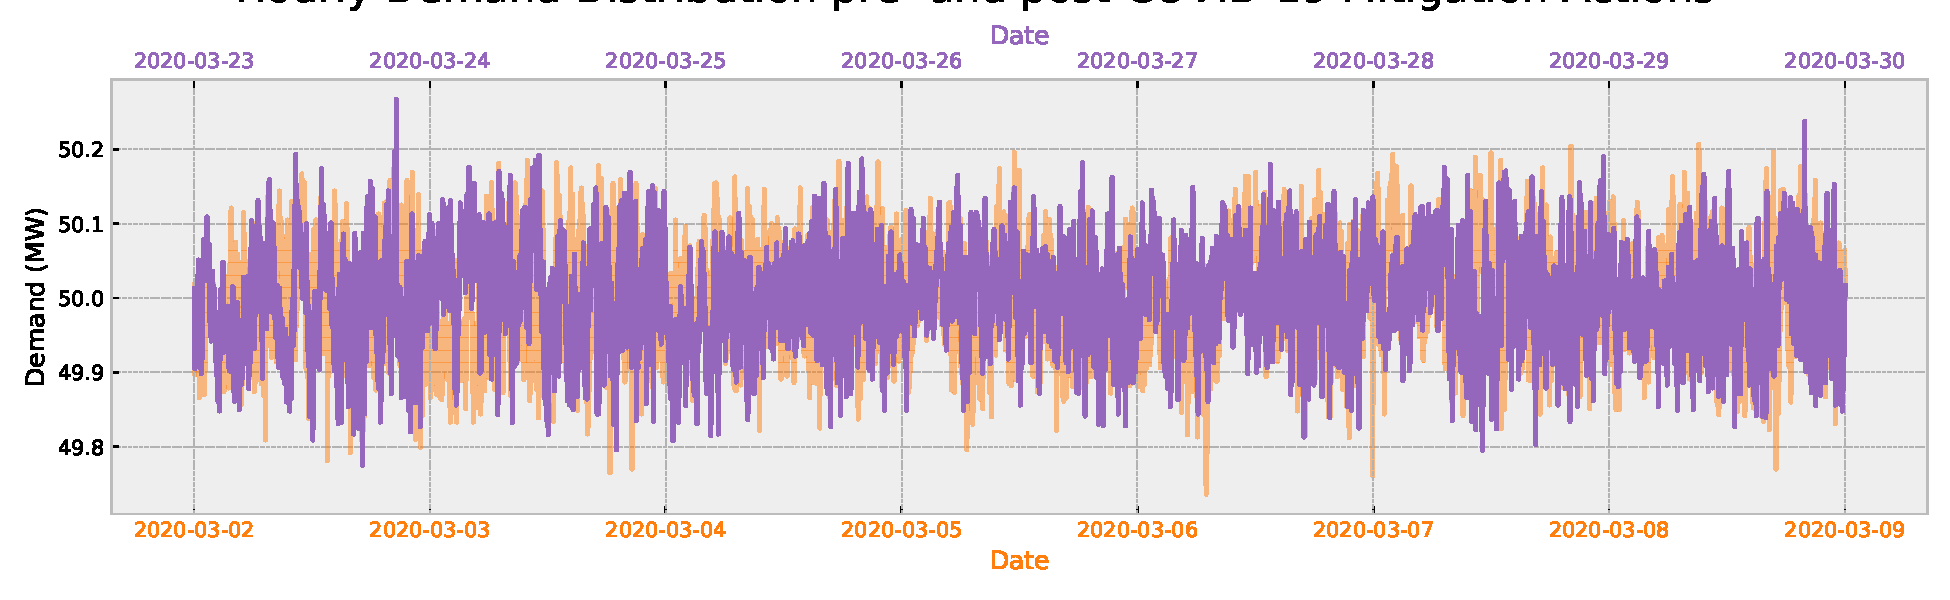
\includegraphics[width=16.5 cm]{Graphics/Freq_pre_post_weekly.pdf}
\caption{Comparison of Pre and Post-action System Frequency  ----- Demand on the left side must be replaced by "Frequency [Hz]" -----} \label{fig:freq_weekly}
\end{figure}  

The Gaussian distribution in Figure \ref{fig:freq_hist}, however, indicates that the highest frequency occurrence changed from below 50 Hz to above 50 Hz at the post-COVID week. ???Not sure. Difference is not really clear as also x-axis changed. Any impacts???

\begin{figure}[H]
\centering

\hspace{-25pt}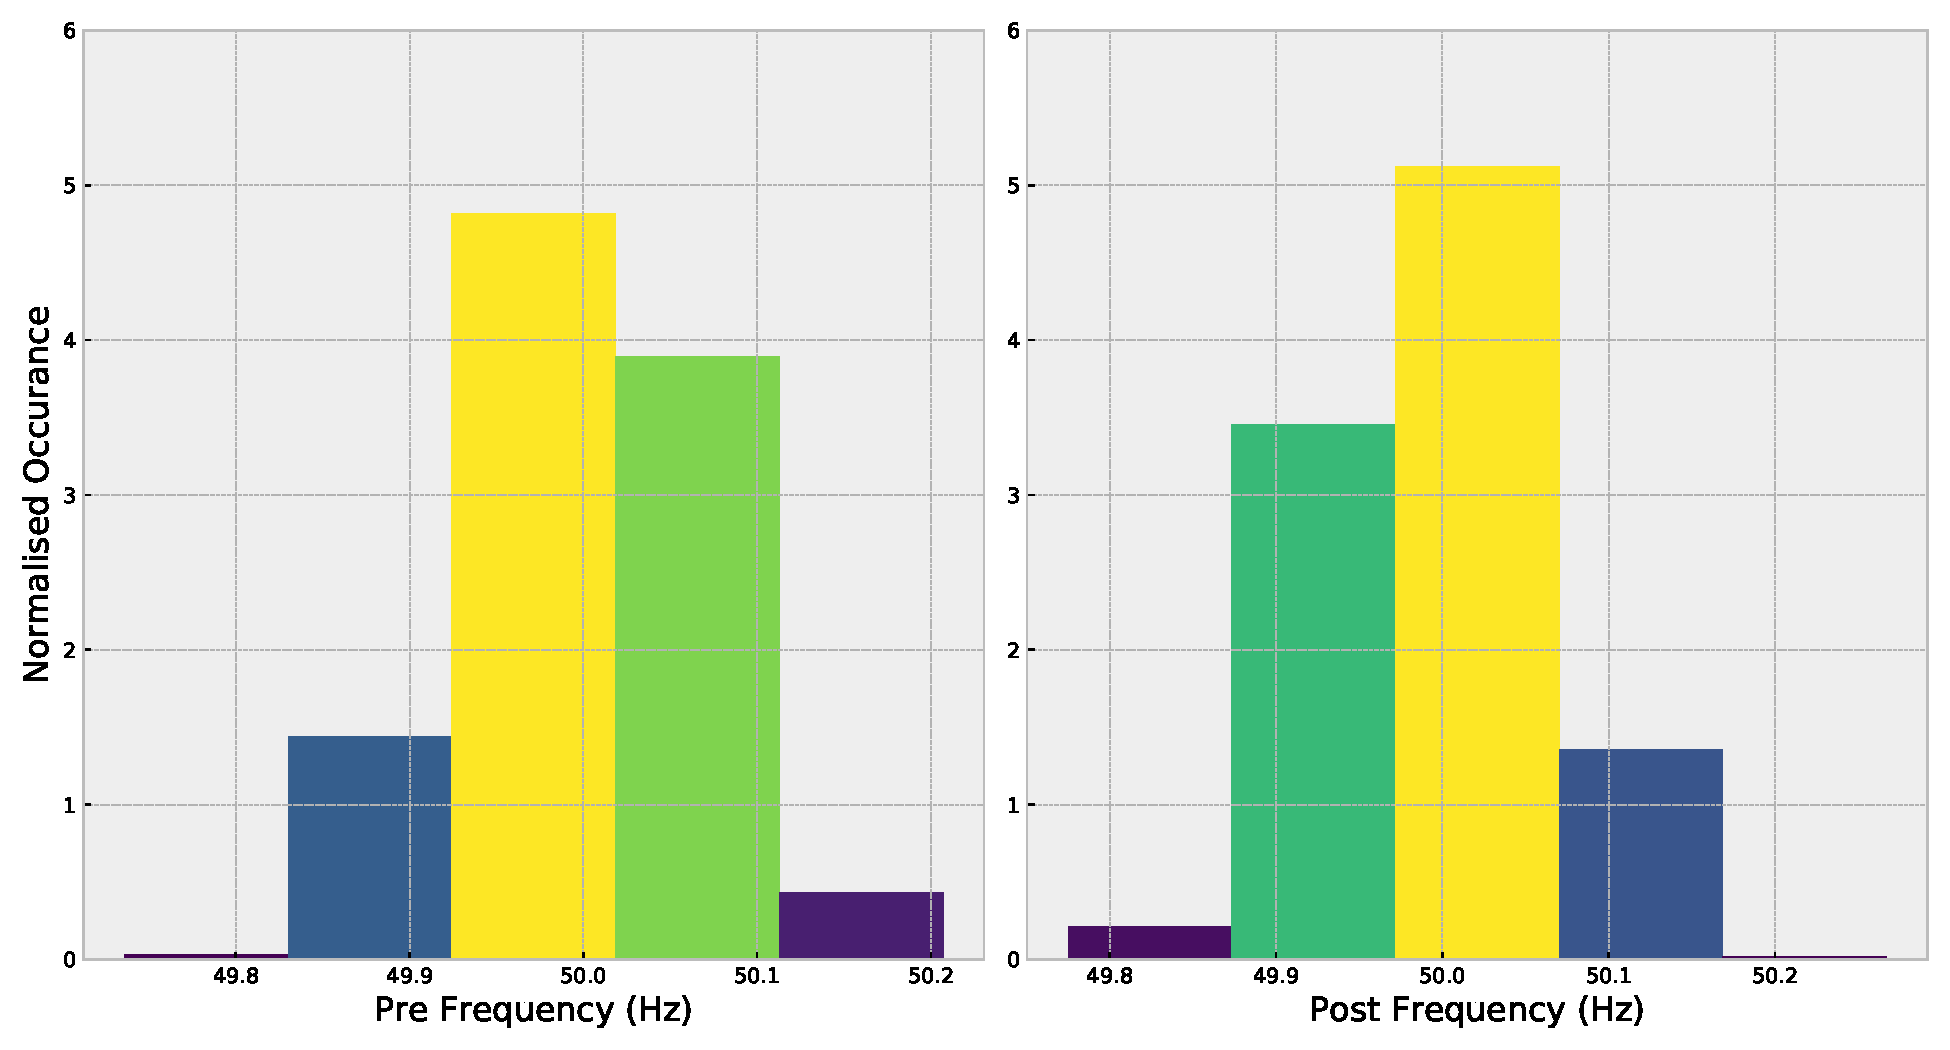
\includegraphics[width=16.5 cm]{Graphics/Freq_hist_side_by_side.pdf}
\caption{Comparison of Pre and Post-action System Frequency Histograms} \label{fig:freq_hist}
\end{figure}  

1. Peak-to-Mean ratio increased during lunch
2. Peak-to-Mean ration increased during "prime time"
3. Peak-to-Mean ratio decreased at night
4. Peak-to-Mean ration decreased in the morning and afternoon
????? INTERPRETATION PARTLY UNCLEAR ????? Prime time indicates more family TV times at 8pm (10 million TV´s equals demand of roughly 7GW)


\begin{figure}[H]
\centering
\hspace{-25pt}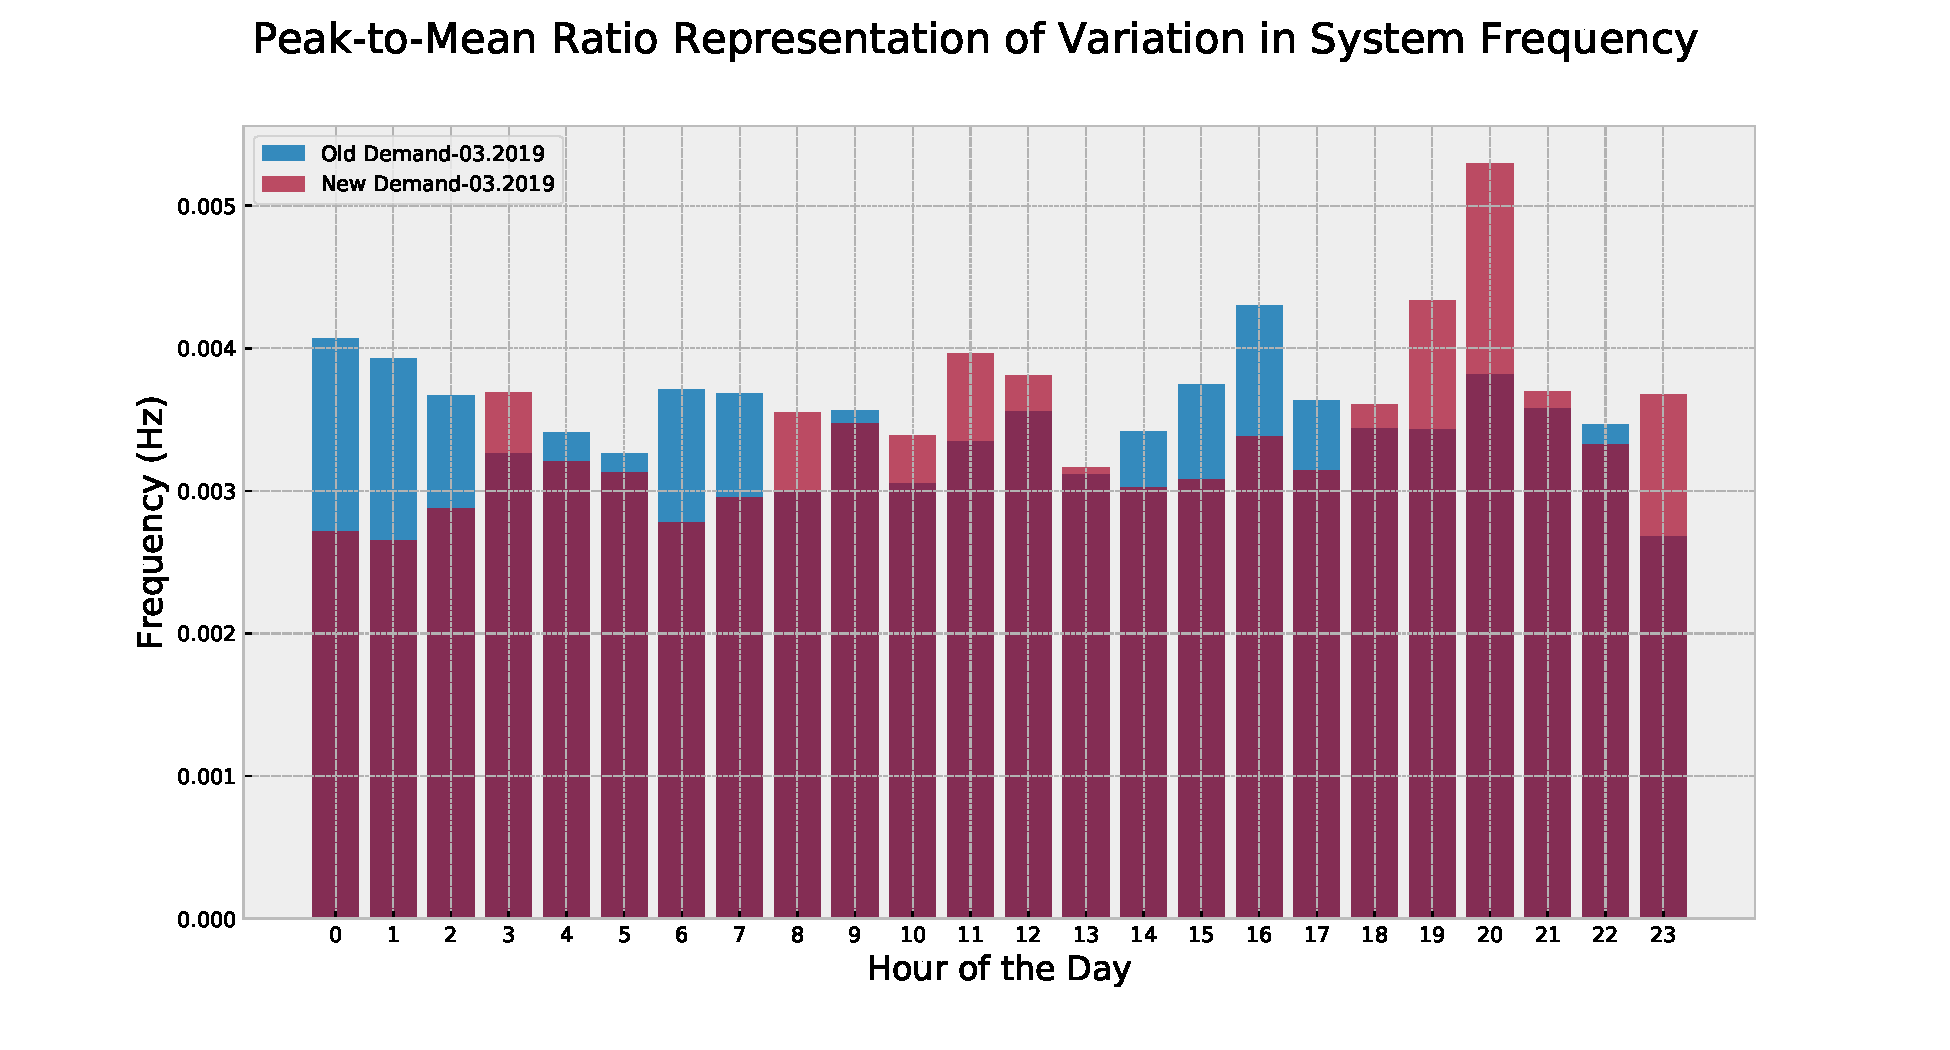
\includegraphics[width=14 cm]{Graphics/Freq_PtM.pdf}
\caption{Comparison of Pre and Post-action System Frequency Peak-to-Mean Ratios} \label{fig:freq_hist}
\end{figure}  

1. Frequency is varying/changing/jumping less on average. Maybe due to the lower peak to base-load ratio ("smoother profile").

\begin{figure}[H]
\centering
\hspace{-25pt}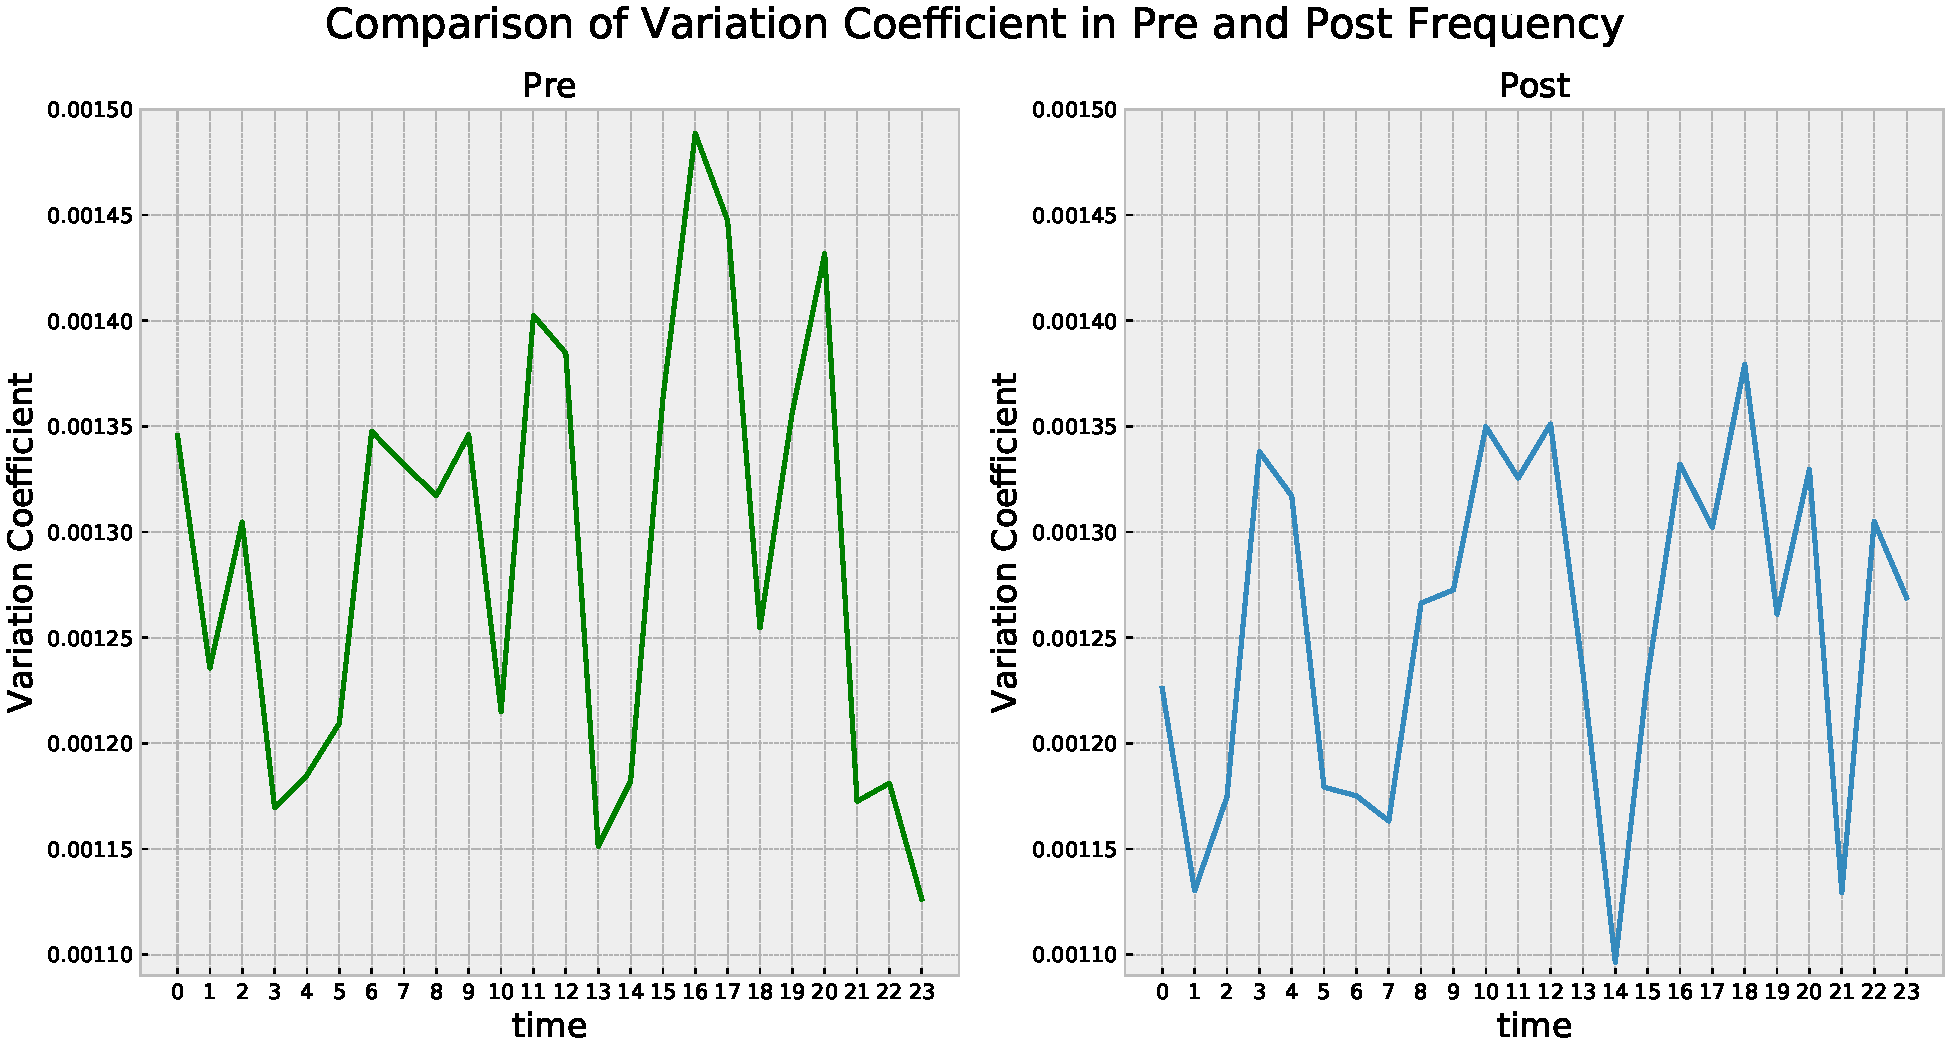
\includegraphics[width=16.5 cm]{Graphics/FFreq_VarCoeff_comp_2.pdf}
\caption{Comparison of Pre and Post-action System Frequency Variation Coefficient} \label{fig:freq_hist}
\end{figure}  

The on average higher share of VRE generation assets (see \ref{generation_effects}) makes the power system more prone for rapid frequency changes \cite{Ela2011OperatingReserves.}. The reason behind this is the change of inertia in the power system. Inertia is provided by conventional synchronous generators, such as in coal, gas, biomass or hydro plants representing spinning masses that store kinetic energy. When for instance, the frequency drops, the rotation of the synchronous generators reduces, providing extra kinetic energy which lowers the supply-demand mismatch or frequency drop. Therefore, a power system with lower inertia, such in case when the share of VRE is high, lead to higher frequency changes in short-term, before any balancing reserve helps out to clear the imbalance. In future, wind and solar power plants could deploy synthetic inertia such described in \cite{Hansen2014AnalysisTurbines, Zeni2013VirtualTurbines, Liu2017PV-basedSystem} to reduce the lack of inertia in VRE dominant power systems.


%Impact of changing generation portfolio on frequency.
%importance of inertia
%generation portofolio and impact intertia
% Sum What the change in inertia will do to the frequency?

%%%%%%%%%%%%%%%%%%%%%%%%%%%%%%%%%%%%%%%%%%%%%%%%%%%%%%%%%%%%%%%%%%%%%%%%%%%%%%%%%%%%%%

\subsubsection{Imbalance Volume}\label{section:ImbalanceVolume}

An imbalance is prevalent in the power system when supply does not match demand. If the imbalance is not tackled, it could lead to an unstable frequency and finally black-outs. It is therefore the System Operators (SO) responsibility to keep the balance in the system \cite{ELEXON2020ELEXONBMRS}. All accepted balancing measures in a settlement period are given by the net imbalance volume (NIV), which represents the total sum of positive and negative system management and energy balancing measure in the settlement period \cite{ELEXON2020ELEXONBMRS}. In a perfect market the power plants are scheduled at gate-closure that demand equals supply at any settlement period to ensure a NIV close to zero. However, the energy balance in a settlement period is usually not met, since \cite{ELEXON2019GuidanceBritain}:
\begin{itemize}
    \item Demand prediction errors by suppliers
    \item Generation prediction errors by generators (i.e. not able to tightly control the operation of intermittent units)
    \item Problems in transmission lines
    \item Balance must exist at every instant, but market trades in half-hour settlement periods 
\end{itemize}

In section \ref{DemandForecastError}, it was recognised the short-length load forecast accuracy decreased slightly. The consequences of this poorer short-length forecast are amplified in the NIV and cause the NIV to grow significantly compared to all other calendar weeks in 2020, see Figure \ref{fig:ImbalanceVolume_over_2020}. Which means whatever changed at the lock-down week, increased the amount and volume of balancing measures in the power system.


\begin{figure}[H]
\centering
\hspace{-25pt}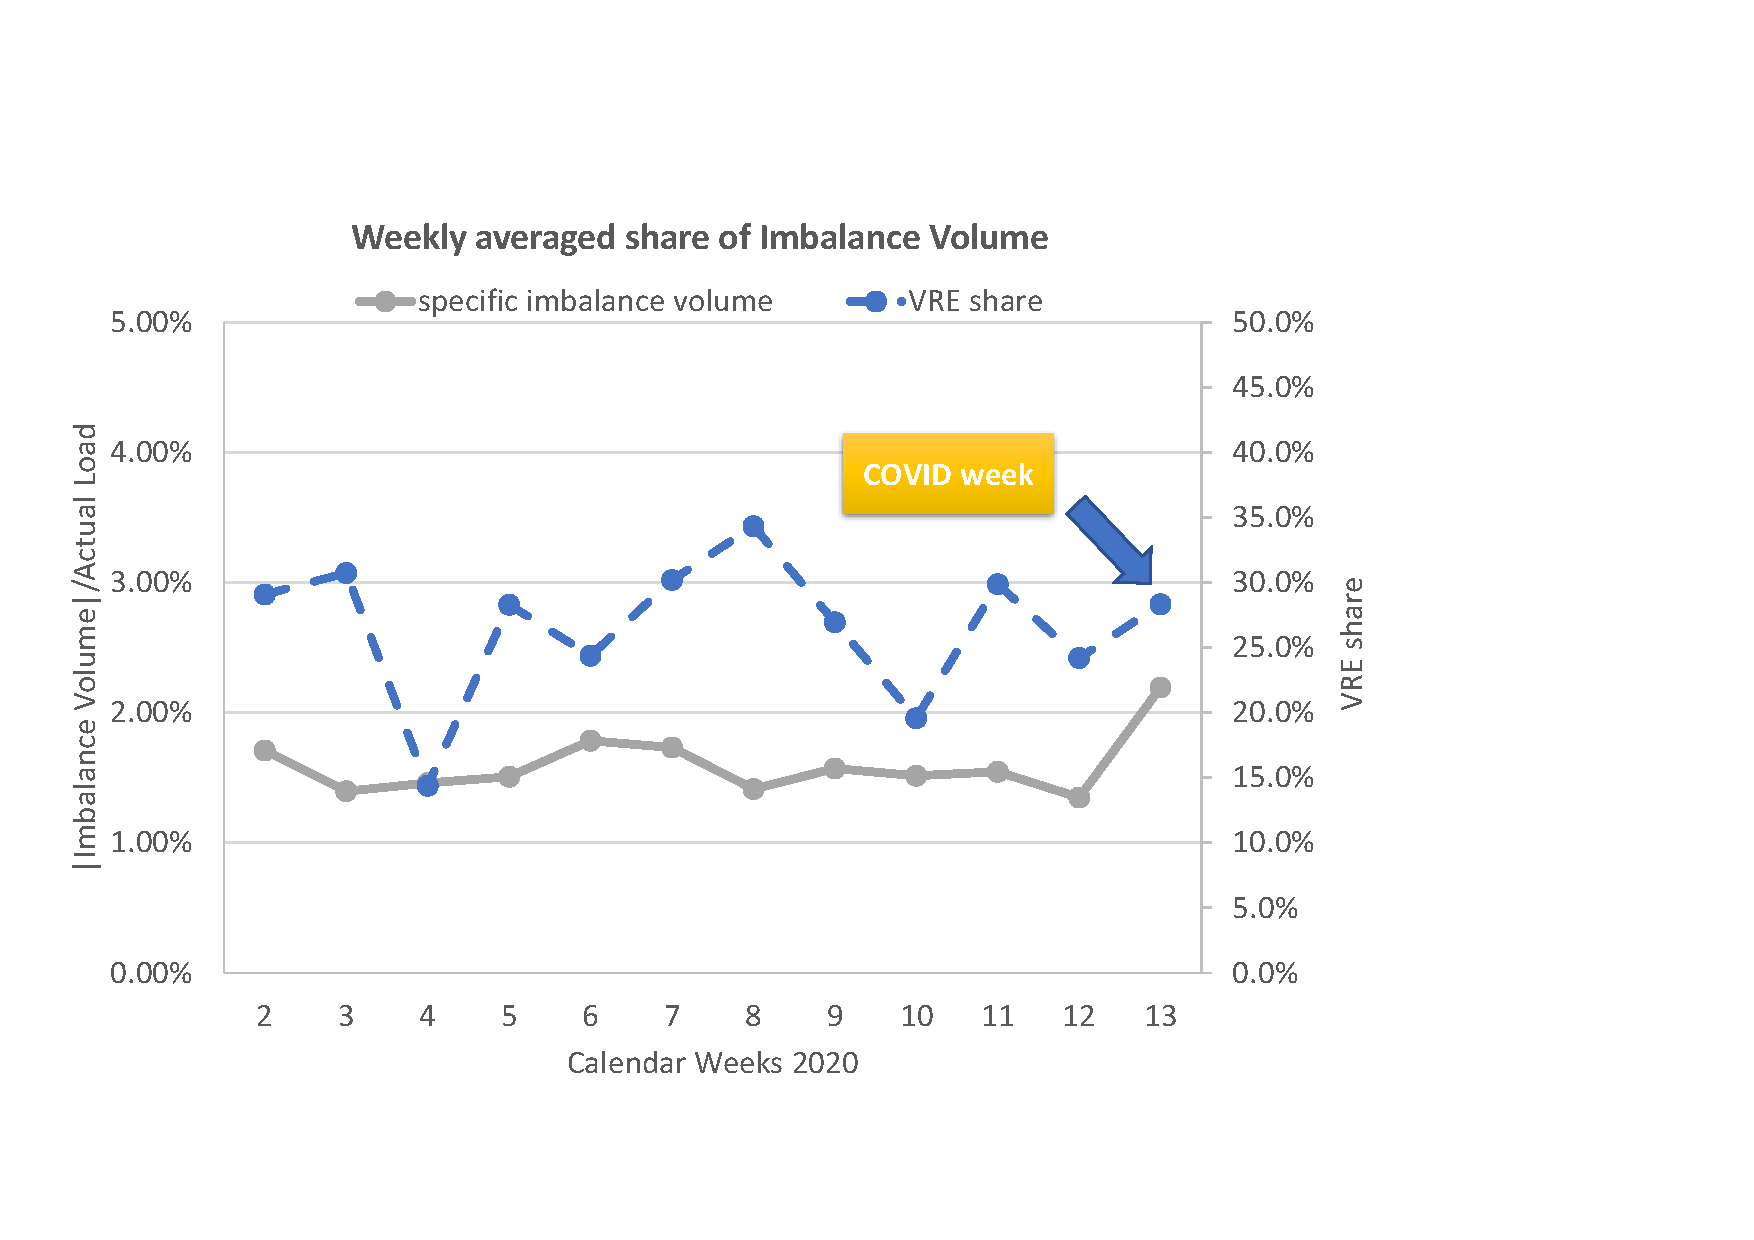
\includegraphics[trim={0cm 2cm 6.5cm 3.5cm},clip,width=0.7\textwidth]{Graphics/Illustration-Imbalance-2020.pdf}
\caption{The weekly average share of imbalance volume factorised by the actual total load. Data from ENTSO-E \protect\cite{ENTSO-E2020ENTSO-EPlatform}}
\label{fig:ImbalanceVolume_over_2020}
\end{figure} 

The higher share of VRE seems to be the main driver for the increasing imbalance in the power system after the lock-down. In Figure \ref{fig:ImbalanceVolume-daily}, the imbalance volume was weighted to the actual total system demand for a pre- and post-COVID week. On the secondary axes is VRE share plotted. Remarkable is the correlation between weighted imbalance volume and the VRE share after the lock-down. The correlation might be not a permanent condition in future. When analysing data from January to March, a correlation between VRE share and imbalance volume was discovered roughly 20\% of the time, though, at approximately 80\% of the time there is no clear correlation visible. Nevertheless, a clear correlation between VRE share and imbalance volume is observed after the lock-down, which indicates that the increasing VRE share is the main driver for the higher imbalance volume. The reason for that cannot be precisely untangled as four things can cause a imbalance, generation and demand prediction errors, network constraints, and the balance need at every instance. 

\begin{figure}[H]
\centering
\hspace{-25pt}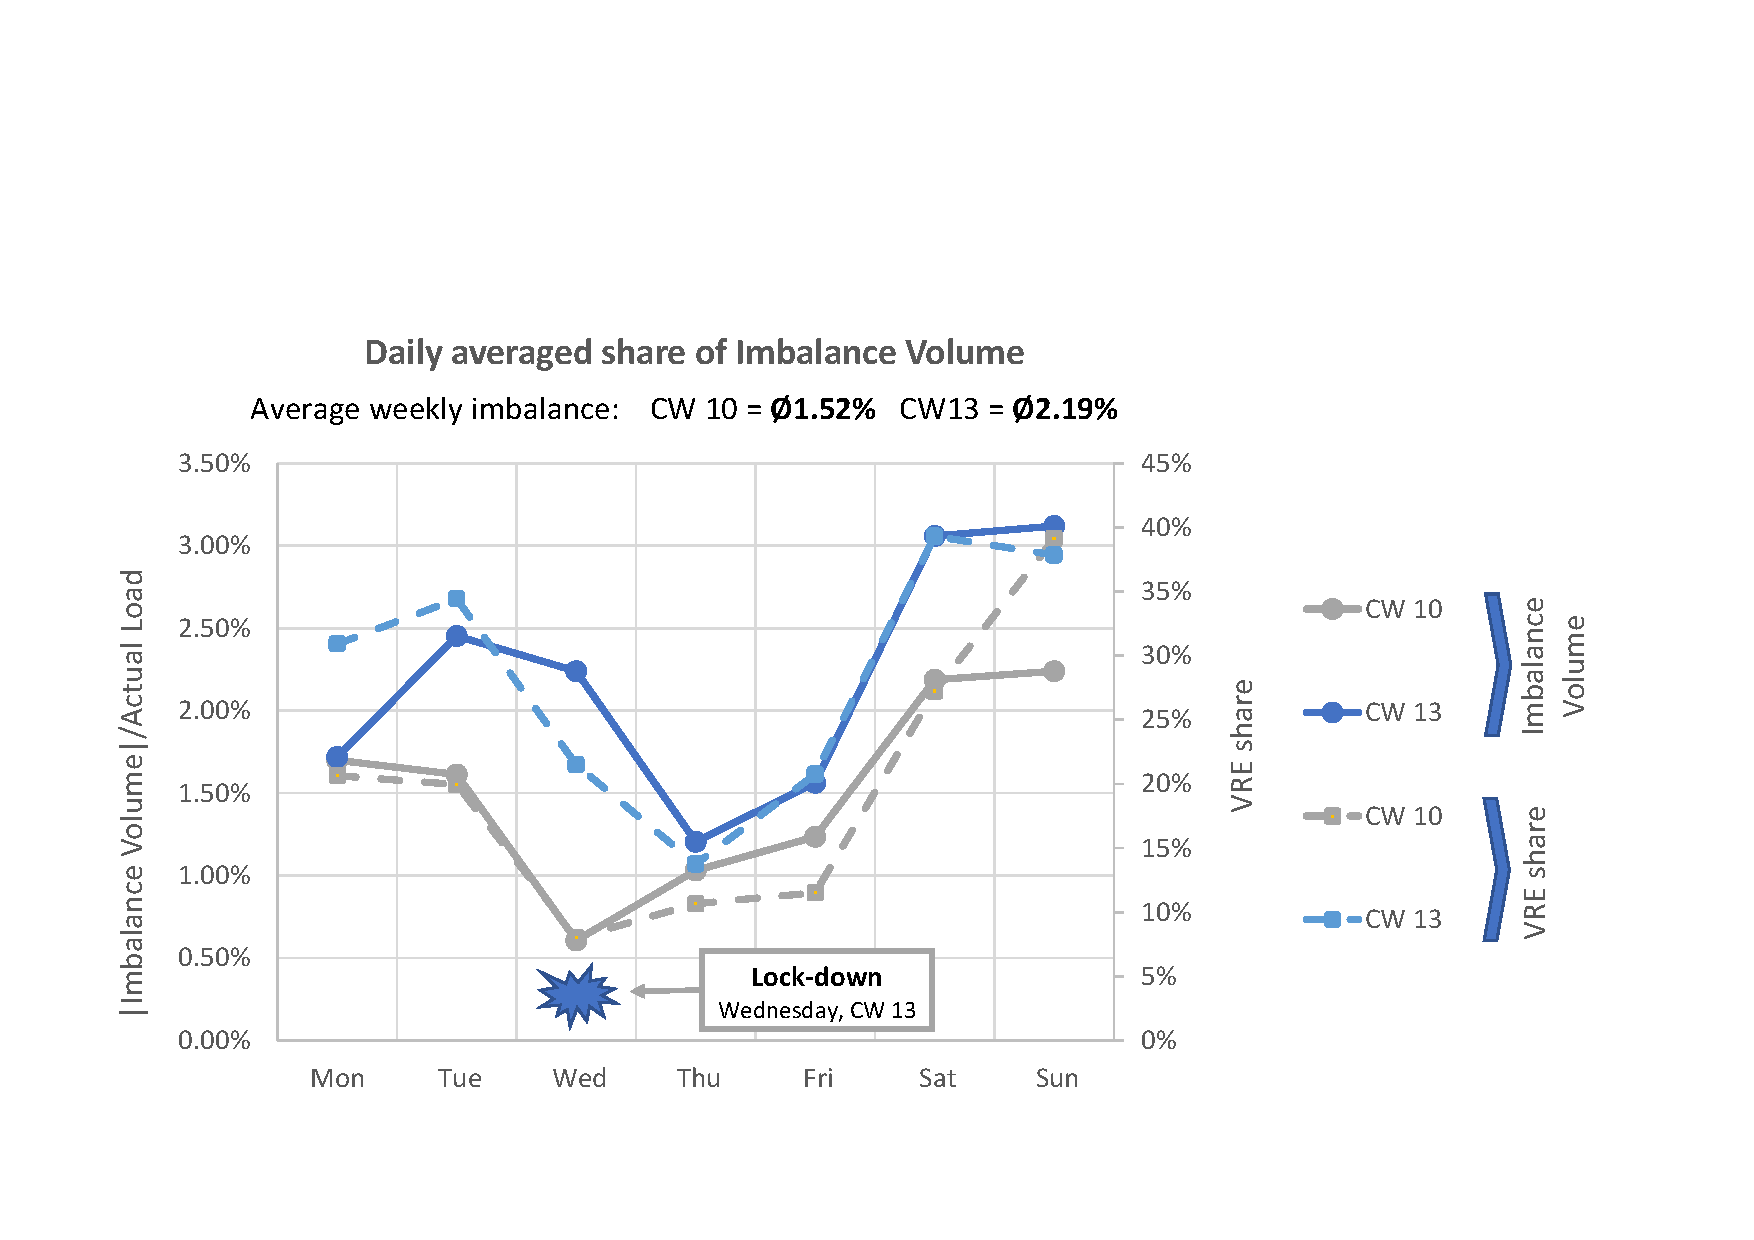
\includegraphics[trim={0cm 2cm 2.5cm 4cm},clip,width=1\textwidth]{Graphics/Illustration-Imbalance-2weeks.pdf}
\caption{Daily average share of imbalance volume and share of VRE for one pre- and post-COVID week, 02-09 March and 22-28 March, respectively. All data available at \protect\cite{ELEXON2020ELEXONBMRS}.}\label{fig:ImbalanceVolume-daily}
\end{figure} 

The effect of higher VRE shares explains the slightly poorer performance of the short-length load forecast TSF, as embedded VRE, which consists of 13 GW solar and 6 GW wind capacity in 2018,  cause load forecast errors \cite{NationalgridESO2018QuarterlyMarch18, NationalGridESO2019EnergyRoadmap}. Contrary, the Day-Ahead load forecast improved, so there might be a trade-off between the benefit of smoother load-profiles and the bad influence of high VRE shares on forecast errors. As summary, it seems that depending on the forecast length, the COVID situation causes improved or worse load forecast performance, see Figure \ref{fig:Illustrative-forecast-summary}. Shorter load forecast-length drop in performance, while longer forecast-length increase in performance.

\begin{figure}[H]
\centering
\hspace{-25pt}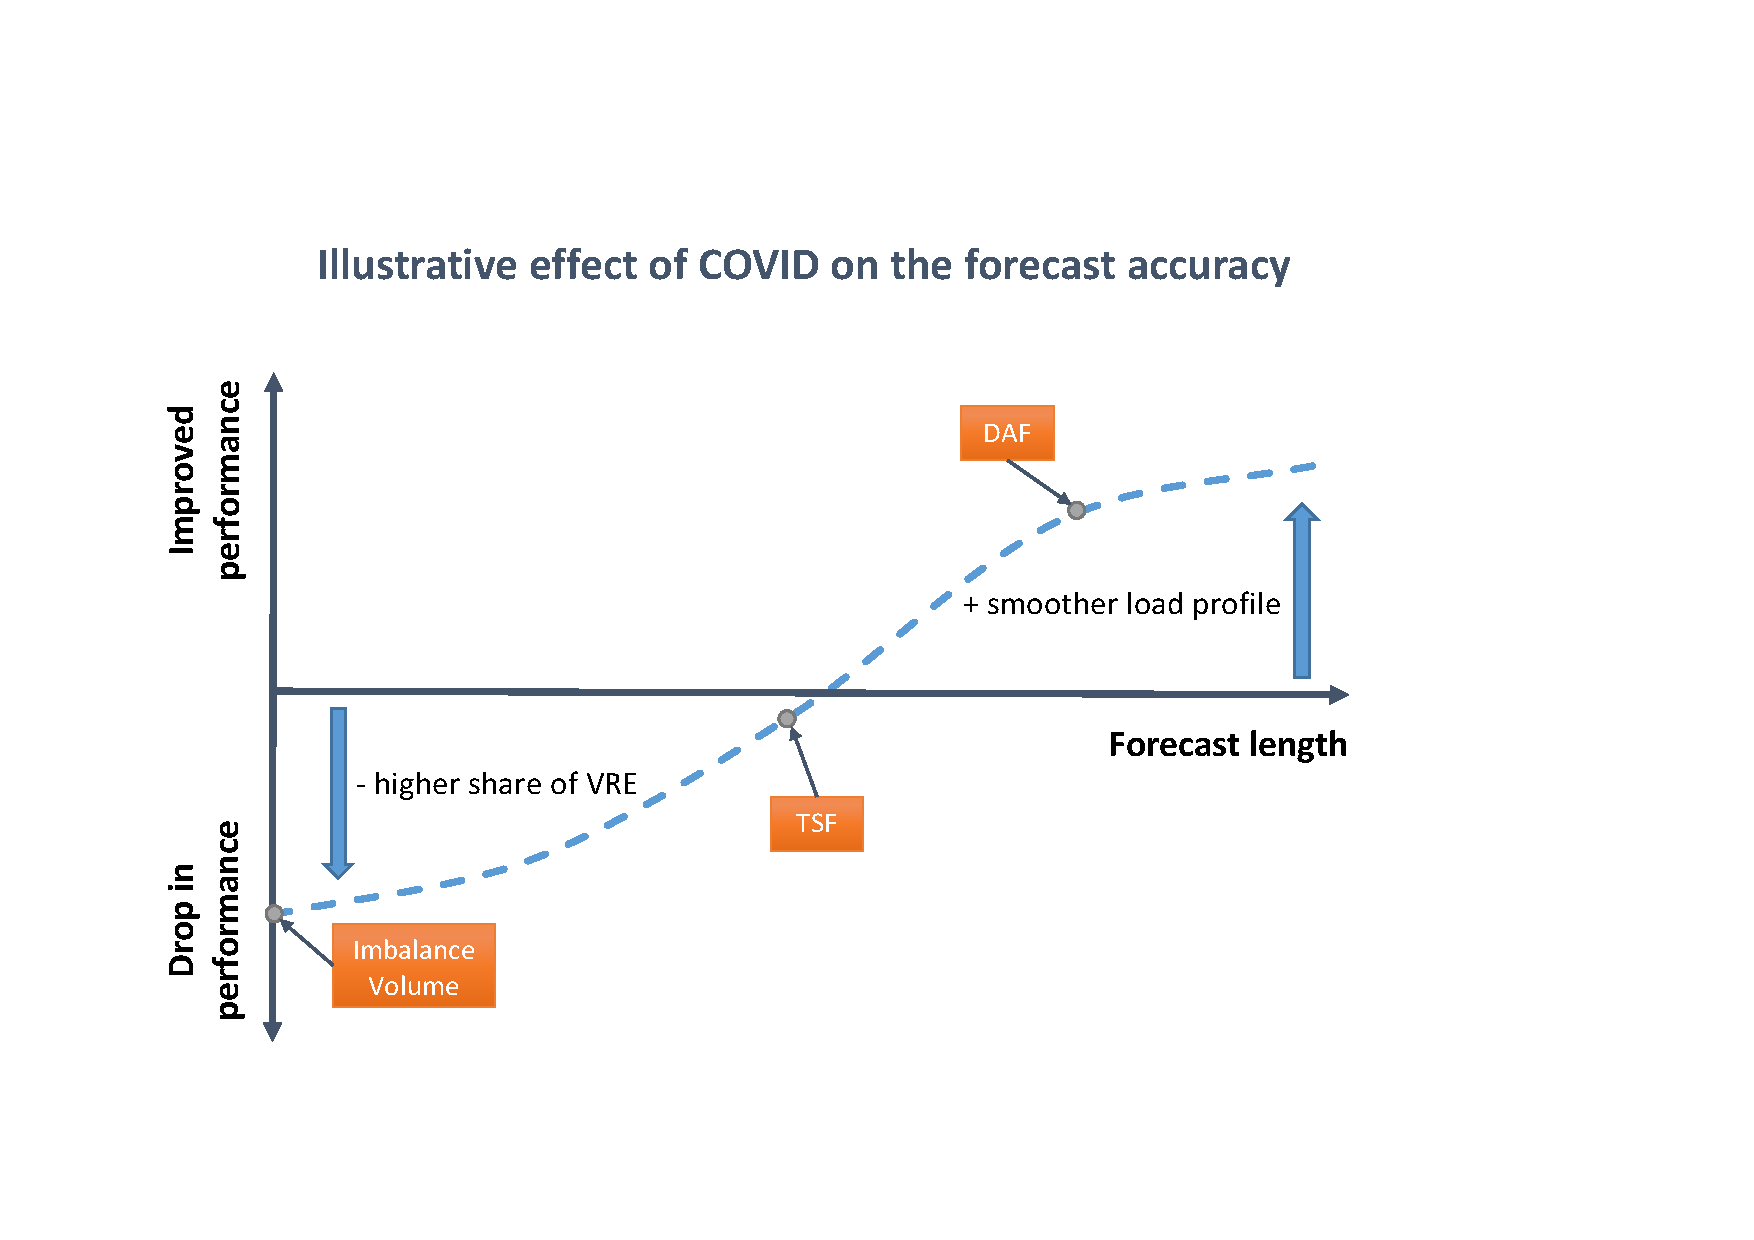
\includegraphics[trim={-1cm 3cm 3cm 3cm},clip,width=1\textwidth]{Graphics/Illustrative-forecast-summary.pdf}
\caption{Illustrative effect of COVID on the forecast accuracy compared to pre-COVID weeks. TSF and DAF indicate the transmission system forecast and total Day-Ahead forecast, respectively, as described in section \ref{DemandForecastError}.}\label{fig:Illustrative-forecast-summary}
\end{figure} 

%%%%%%%%%%%%%%%%%%%%%%%%%%%%%%%%%%%%%%%%%%%%%%%%%%%%%%%%%%%%%%%%%%%%
\subsubsection{LOLP \& DRM}\label{section:LOLP_DRM}

Loss of load probability (LOLP) is an indicator for system reliability measured by the system operator for each settlement period \cite{ELEXON2019GuidanceBritain}. For instance, when National Grid predicts higher probability of loss of load, the balancing mechanism is willing to pay higher prices for balancing at the time of reserve scarcity. The methodology to calculate the LOLP can be found in \cite{Elexon2019LossStatement}. The higher prices at high LOLP levels are also known as reserve scarcity prices, which are the product of LOLP and the value of lost load (VoLL). Whereby, the VoLL is determined through the assessment of how much value consumers on average attribute to the security of supply - currently set on £6000/MWh \cite{ELEXON2019GuidanceBritain}. 

\[ \text{Reserve Scarcity Price} = \text{Lost of Load Probability} * \text{Value of Lost Load} \]

Due to the abrupt changes in the demand profile and eventually the inflexibility of the available generation, National Grid predicted a higher LOLP during the evening of the 25th of March which is the first official day of lock-down (see Figure \ref{fig:LOLP_25_03}. Despite the fact that it was predicted 12 hours in advance, the 1 hour ahead LOLP forecast is 4.5 times higher. This implies that there was a reserve scarcity and/or that the grid was under stress.

\begin{figure}[H]\centering
\hspace{-25pt}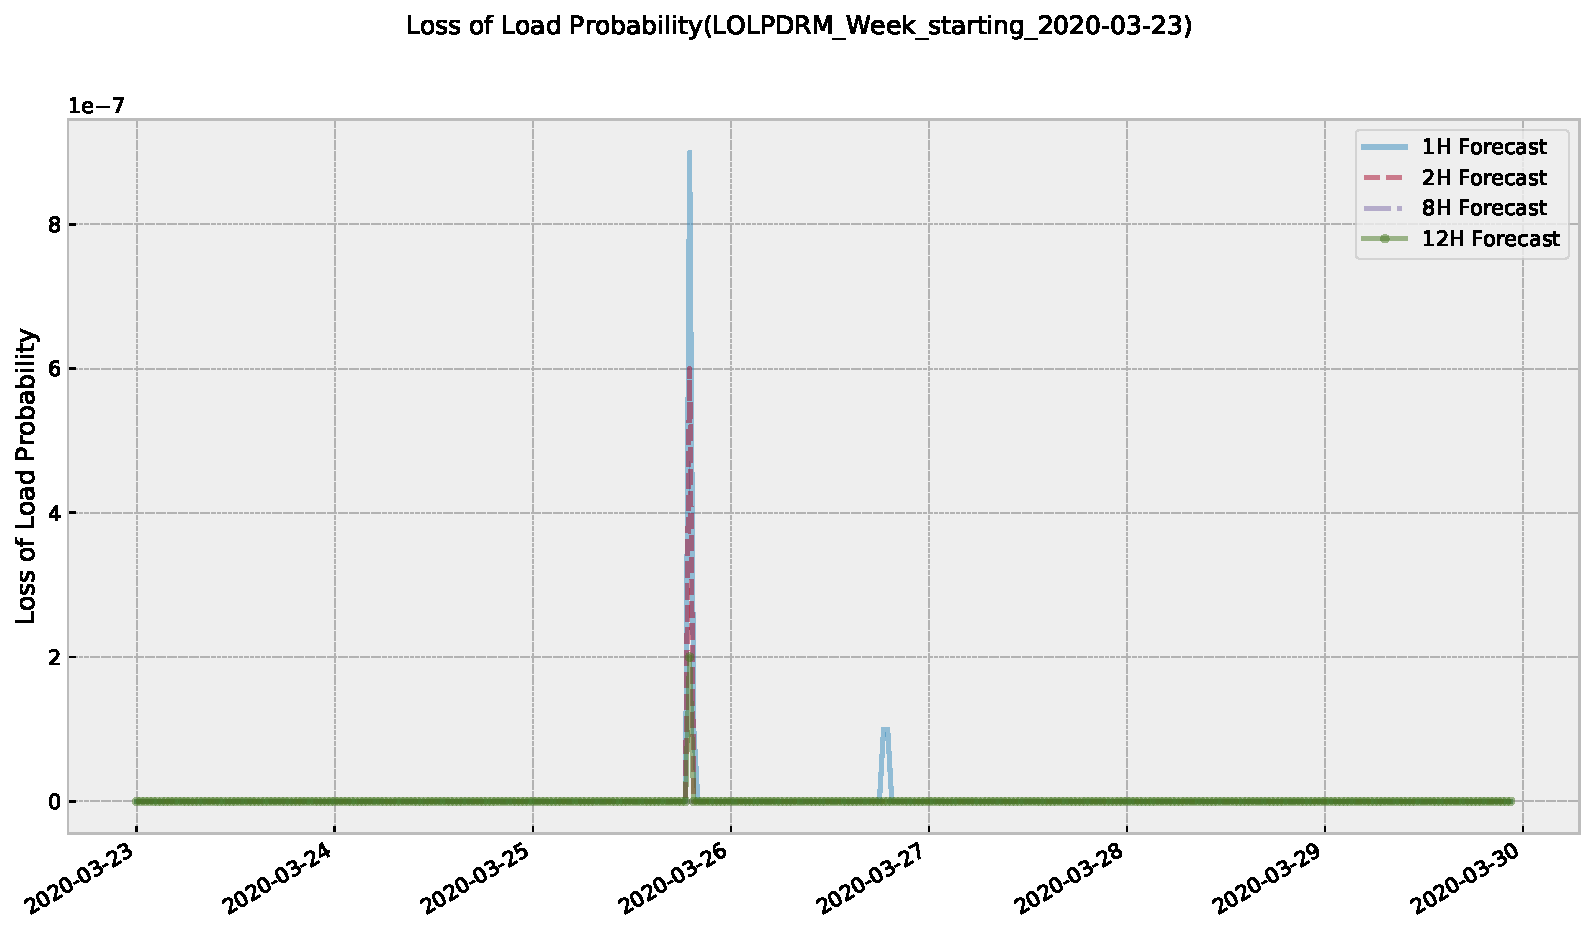
\includegraphics[width=15 cm]{Graphics/LOLPDRM_Week_starting_2020-03-23no4H.pdf}
\caption{LOLP variation Pre and Post.}\label{fig:LOLP_25_03}
\end{figure}  


%%%%%%%%%%%%%%%%%%%%%%%%%%%%%%%%%%%%%%%%%%%%%%%%%%%%%%%%%%%%%%%%%%%%%%%%%%%%%%%%
%\subsection{Ancillary Services/Demand-side Response}
%%%%%%%%%%%%%%%%%%%%%%%%%%%%%%%%%%%%%%%%%%%%%%%%%%%%%%%%%%%%%%%%%%%%%%%%%%%%%

\subsection{The effects on Market Price}\label{section:Market price}

%%%%%%%%%%%%%%%
\subsubsection{Day-Ahead wholesale market price}\label{sec:day-ahead wholesale market price}

The Day-Ahead market objective is to define a clearing energy price in which supply meets the demand at any given hour of the day. To do so, a merit order model is used to correctly dispatch power plants by sorting the existing generation units from low to high marginal operating costs. Once the generation meets the demand curve the clearing market price or equilibrium is achieved by minimising the generation cost \cite{Maekawa2018TheExchange}. Figure \ref{fig:wholesale-market-effects} shows graphically the process of the merit order model and the location of the clearing price as a result of the intersection of the supply and demand curves. The demand is given as net demand which subtracts the VRE generation from the total demand. This is a common strategy to illustrate the merit-order, since the solar and wind generation plants have marginal cost close to zero, making them always dispatched so far no network or other operational constraints exist \cite{Hirth2014TheVariability}. 

\begin{figure}[H]
\centering
\hspace{-25pt}
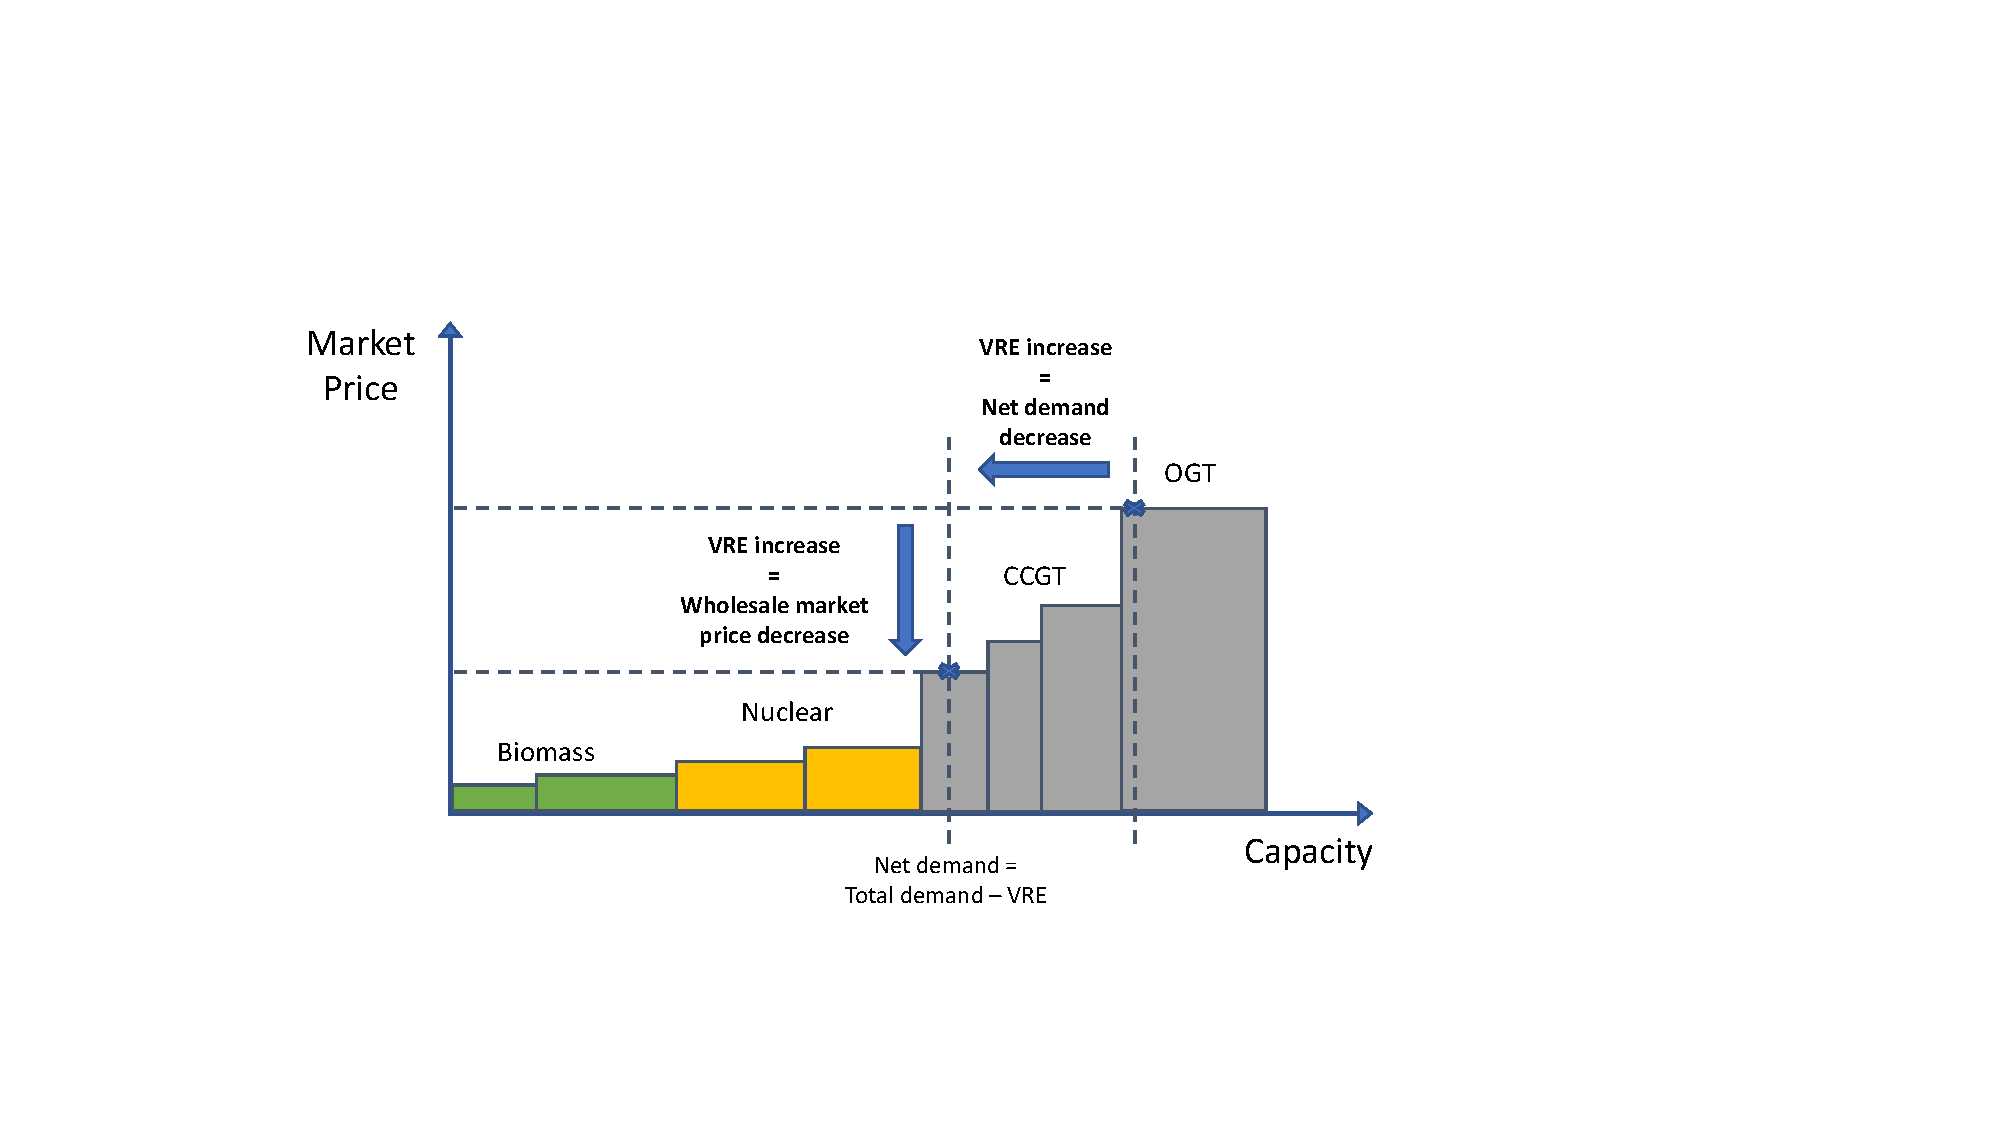
\includegraphics[trim={4cm 3cm 3.5cm 4.5cm},clip,width=1.3\textwidth]{Graphics/Wholesale-market-price.pdf}
\caption{Illustrative effects of the COVID-situation on the wholesale market price.}
\label{fig:wholesale-market-effects}
\end{figure} 


\subsubsection{System imbalance price}\label{sec:system imbalance price}

The imbalance price is the price set by the system operator for every settlement period to determine imbalance charges on electricity producers (generators) or consumers (suppliers) \cite{ELEXON2019GuidanceBritain}. Whereby the imbalance charge for a settlement period simply consist of the product of imbalance volume (see section \ref{section:ImbalanceVolume}) and imbalance price:

\[ \text{Imbalance charge}_{SP} = \text{Imbalance volume}_{SP} * \text{Imbalance price}_{SP} \]

To understand possibles impacts of the COVID situation on the imbalance price, it dismantled in its components. The imbalance price is the price which must be paid for actions that the system operator choose to resolve the imbalance. However, the reason for the balancing action can vary. It could be either a i) energy balancing or ii) system balancing motivated action in the 30min settlement period \cite{ELEXON2019GuidanceBritain}. 

According to \cite{ELEXON2019GuidanceBritain}, the energy balancing action in the "Balancing Mechanism"(BM) make sure that the energy amount of the physical notification is accomplished. This type of balancing action is usually priced by Bid-Offer scheme. The merit-order wise choice of Bid-Offers, meaning cheap actions first, is preferred to reduce the balancing cost. Though, this is not always possible due to technical limitations of generators, demands and networks. An example for a technical limitation of a BM-generator is a non-suitable ramp-up rate, or a limitation for the network, an already congested line which would not allow more generation. Therefore, not only the cheapest BM Bid-Offer prices are selected or resolved by the system operator. In the BM, units are usually priced by the utilisation cost, however, short term operating reserves (STOR) take a special role for the stability and priced by the greater price between i) utilisation price or ii) reserve scarcity price. Whereby, the reserve scarcity price is the product of the Loss of Load Probability (LoLP) and Value of Lost Load (VoLL). 

For the purpose of energy balancing, the system operator might additionally purchase non-BM services as "Balancing Service Adjustment Action" \cite{Nationalgrid2017ProcurementSO}. Drivers for such an adjustment action could be a more economical or specific necessary balancing characteristics from non-BM services, such as ancillary services or "other services" according to \cite{Nationalgrid2018BalancingStatement}. These non-BM actions are priced in capacity or energy or both ways and form balancing service adjustment data, consists of adjusted buy and sell prices, which adjust the imbalance price of the previously described BM \cite{Nationalgrid2017ProcurementSO,Nationalgrid2018BalancingStatement}.

The system-balancing actions, otherwise, are only a part of the non-BM actions \cite{Nationalgrid2018BalancingStatement}. They describe balancing actions which keep the energy balance at every instance. For example, a wind power plant might generate the exact energy amount as contracted by the physical notification for the 30 min settlement period, however, its power might fluctuate and mismatch the demand in the settlement period which make system-balancing actions, such as activation's of non-BM STOR units, necessary \cite{Nationalgrid2018BalancingStatement}. The pricing scheme for the system-balancing actions is equal to the energy-balancing scheme for non-BM actions, described in the previous paragraph.  

Figure \ref{fig:imbalance-price-development}, illustrates the weekly averaged imbalance price development in 2020. The imbalance price dropped significantly in the first week of the lock-down, while increased in the following week significantly. As described in the above paragraphs, the imbalance price is a complex construct. As result, the impact of the lock-down on the imbalance price can just be qualitatively evaluated.

\begin{figure}[H]
\centering
\hspace{-25pt}
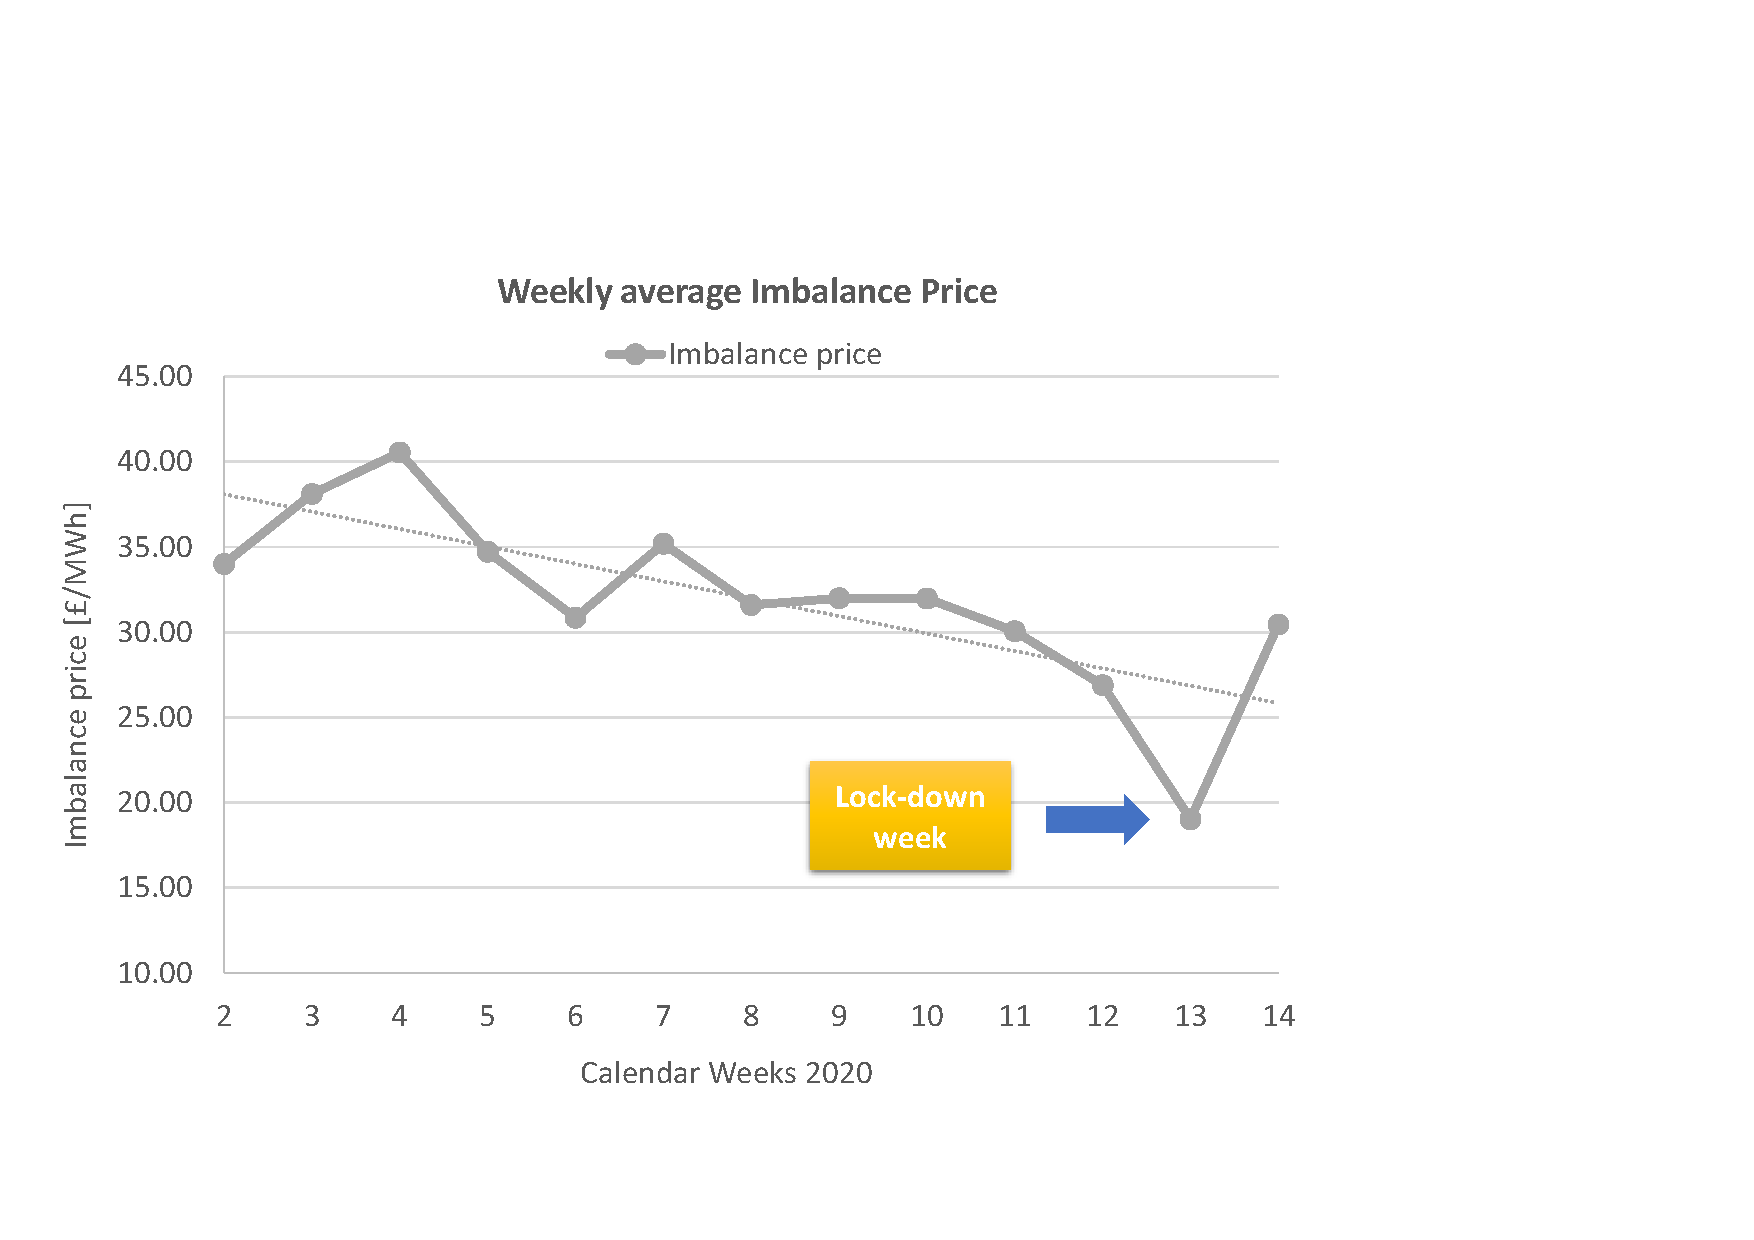
\includegraphics[trim={0cm 2cm 7cm 4.5cm},clip,width=0.8\textwidth]{Graphics/Imbalance-price-development-2020.pdf}
\caption{The impact of lower demand on the imbalance price}
\label{fig:imbalance-price-development}
\end{figure} 

The impacts of the lower demand at the lock-down times could both potentially increase and lower the imbalance price (see Fig. \ref{fig:imbalance-price-trade-off}). The balancing service options are generally chosen in a merit-order wise way, meaning activating cheap options first, if no system operation limitation exists. Therefore, similar to a the wholesale market price settling, a higher demand would lead to higher prices, vice versa, cheaper generation would lower the price. That the imbalance volume could increase was explored in section \ref{section:ImbalanceVolume}. Moreover, an on average lower demand as discovered in \ref{section: Effect on demand profile}, would potentially free up more generation units that can provide additional cost-effective balancing services. The described effects frame not the whole picture, additionally investigation could be made on the LoLP, the VoLL, the De-rated Margin, voltage related services and the network utilisation.

\begin{figure}[H]
\centering
\hspace{-25pt}
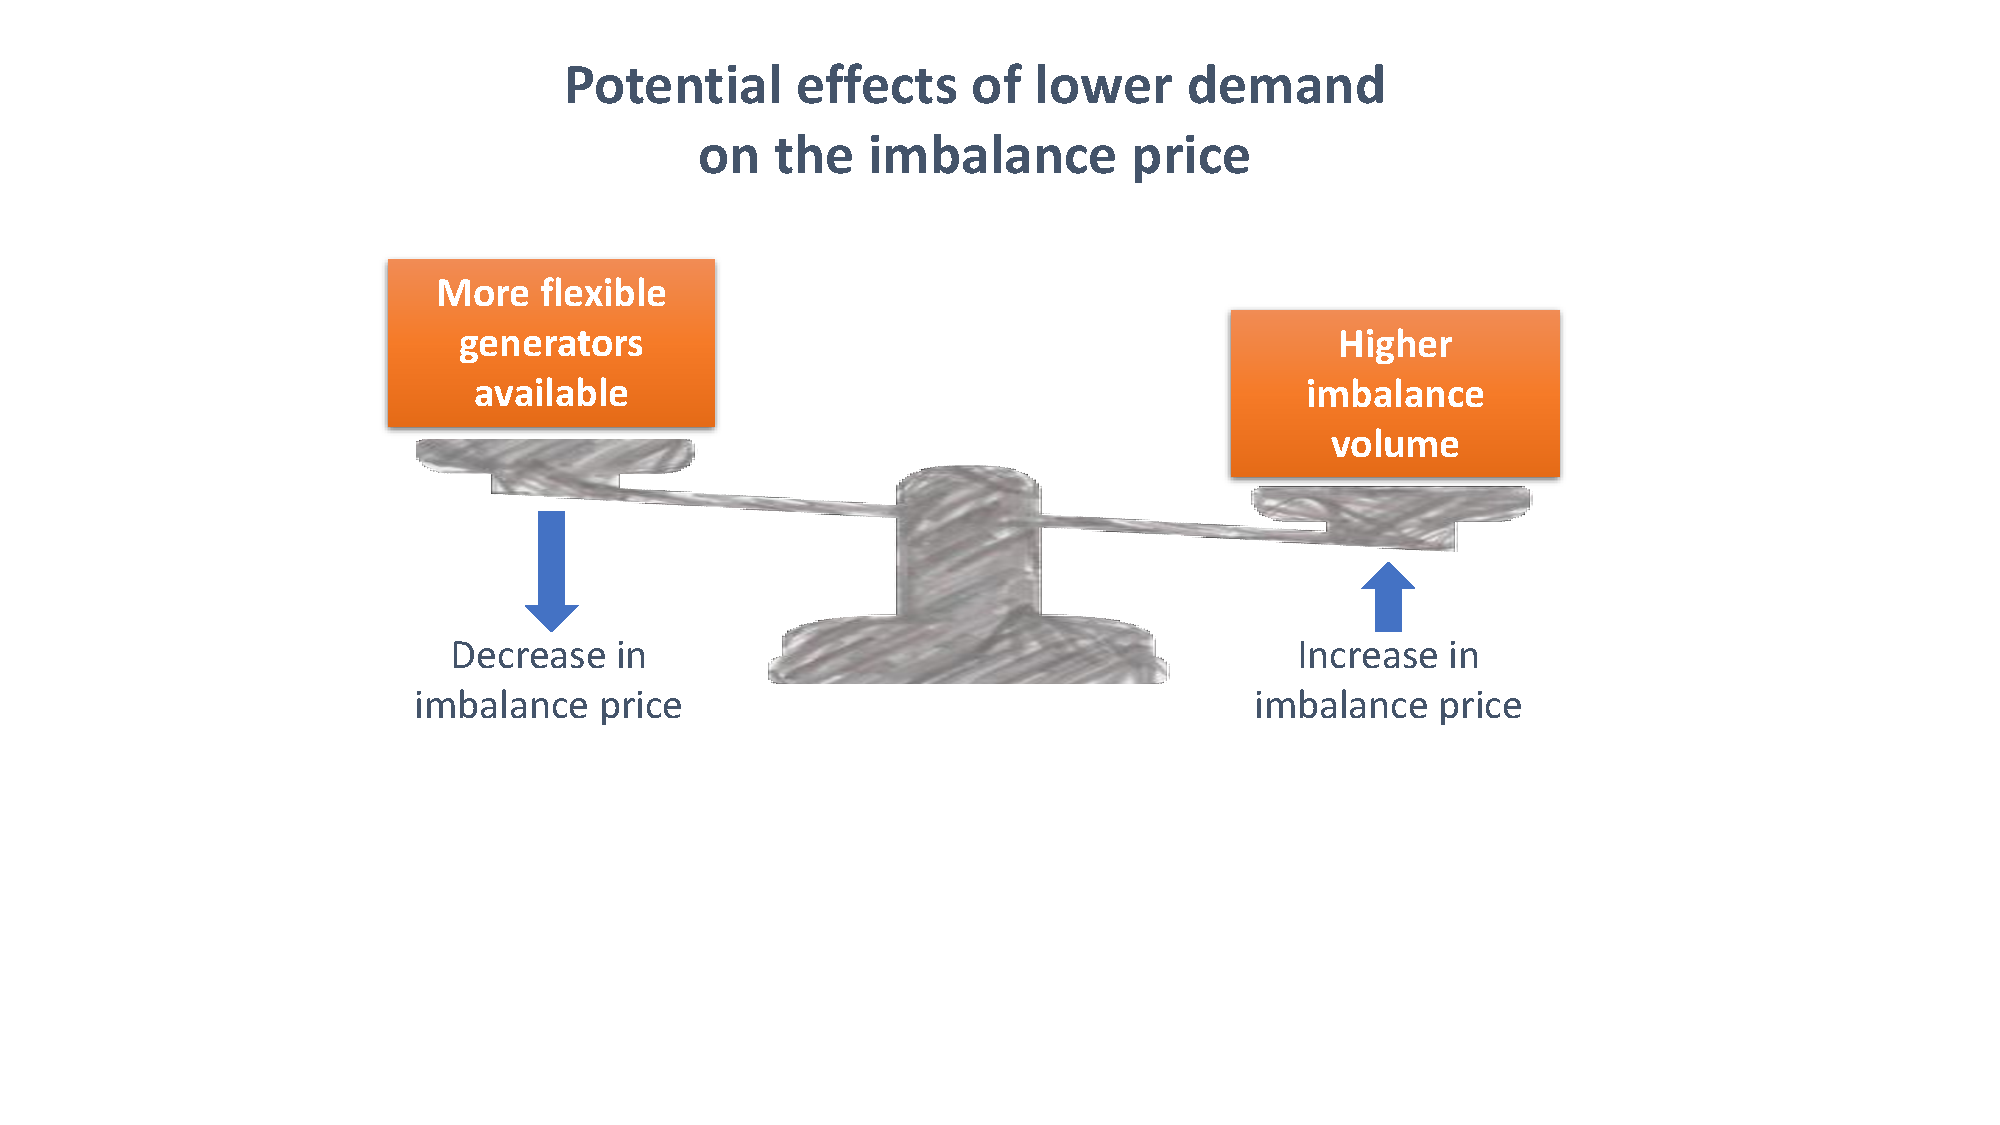
\includegraphics[trim={4cm 6.3cm 5cm 1cm},clip,width=1\textwidth]{Graphics/Imbalance-price-trade-off.pdf}
\caption{The impact of lower demand on the imbalance price}
\label{fig:imbalance-price-trade-off}
\end{figure} 


%De-rate margin would be helpful.
%What is De-Rated Margin?De-rated Margin is a measure of the excess supply on the system, which has been adjusted to take account of the likely availability of plant, specific to each type of generation technology. %%%%"It reflects the proportion of an electricity source which is likely to be technically available to generate when needed"%%%%

%energy imbalance price calculation based on a theoretical set of balancing actions

%SO does not take all balancing actions for the same reason. 
%Some balancing actions are taken purely to balance the half hour energy imbalance of the Transmission System. These are ‘energy balancing’ actions.Other balancing actions are taken for non-energy, system management reasons. These are ‘system balancing’ actions.

%There are two energy imbalance prices for each Settlement Period. These are:System Buy Price (SBP); and System Sell Price (SSP).However there is a single price calculation, so SBP will equal SSP in each Settlement Period. ELEXON apply these prices to Parties’ imbalances to determine their imbalance charges. A Party is out of balance when its contracted energy volume does not match its physical production orconsumption.

\subsubsection{Agile Pricing}
A British energy supplier called Octopus \cite{AgileEnergy} introduced their "Agile" electricity tariff in which is an indexed half-hourly dynamic pricing that tracks the wholesale price of electricity (i.e. the domestic rate paid changes every 30 minutes instead of a fixed monthly rate). On different occasions, this has resulted in negative pricing (i.e. the energy supplier paid its customers use electricity). However, this also means that there is usually a steep price from 4pm to 7pm during the evening consumption peak. The following logic in Eq. \ref{eq:Octopus}, is used to determine the prime time pricing. It uses the of the distribution cost coefficient ($\tau$) multiplied by the wholesale cost of electricity ($W$) and $P$ which is the peak-time premium (which is equal to 12p/kWh during prime time). Then it caps the price to £35p/kWh if the previous outcome is higher than this value. This is because on average the fixed tariff are in the range of 15-20p/kWh and it could be argued exposing domestic consumers to extreme fluctuations in the system would be unfair.

\begin{equation}\label{eq:Octopus}
min((\tau \times W + P), 35p/kWh)
\end{equation}

Octopus GO


\begin{figure}[H]\centering
\hspace{-25pt}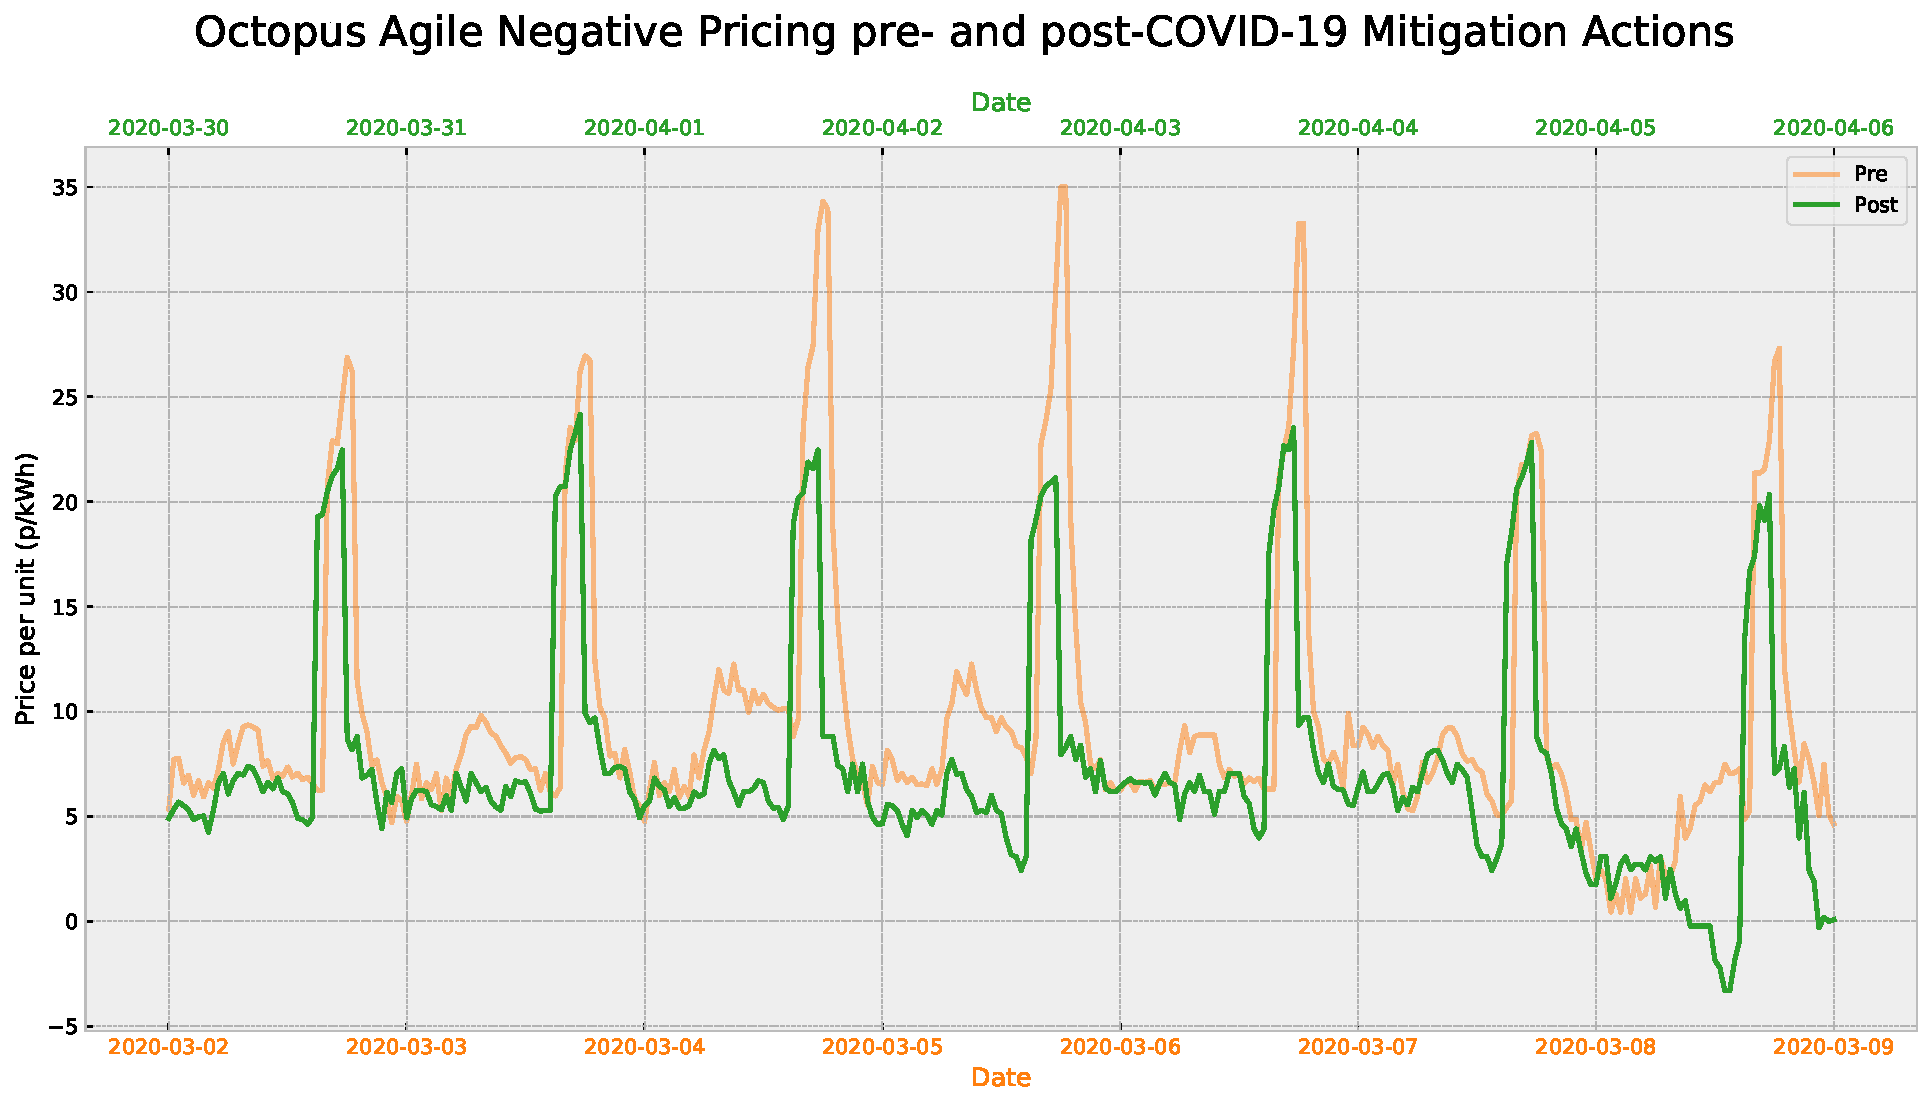
\includegraphics[width=15 cm]{Graphics/Pre-post_Agilecomp_negative.pdf}
\caption{Negative electricity pricing - 4th March was the highest }\label{fig:neg_agile_comp_prepost}
\end{figure}  

The Balancing Mechanism System Price peaked at £2,242/MWh on the 4th of March 2020 which marks the first time a system price is over £2,000/MWh since 2001 \cite{ELEXON2020ELEXONBMRS}. 

\begin{figure}[H]\centering
\hspace{-25pt}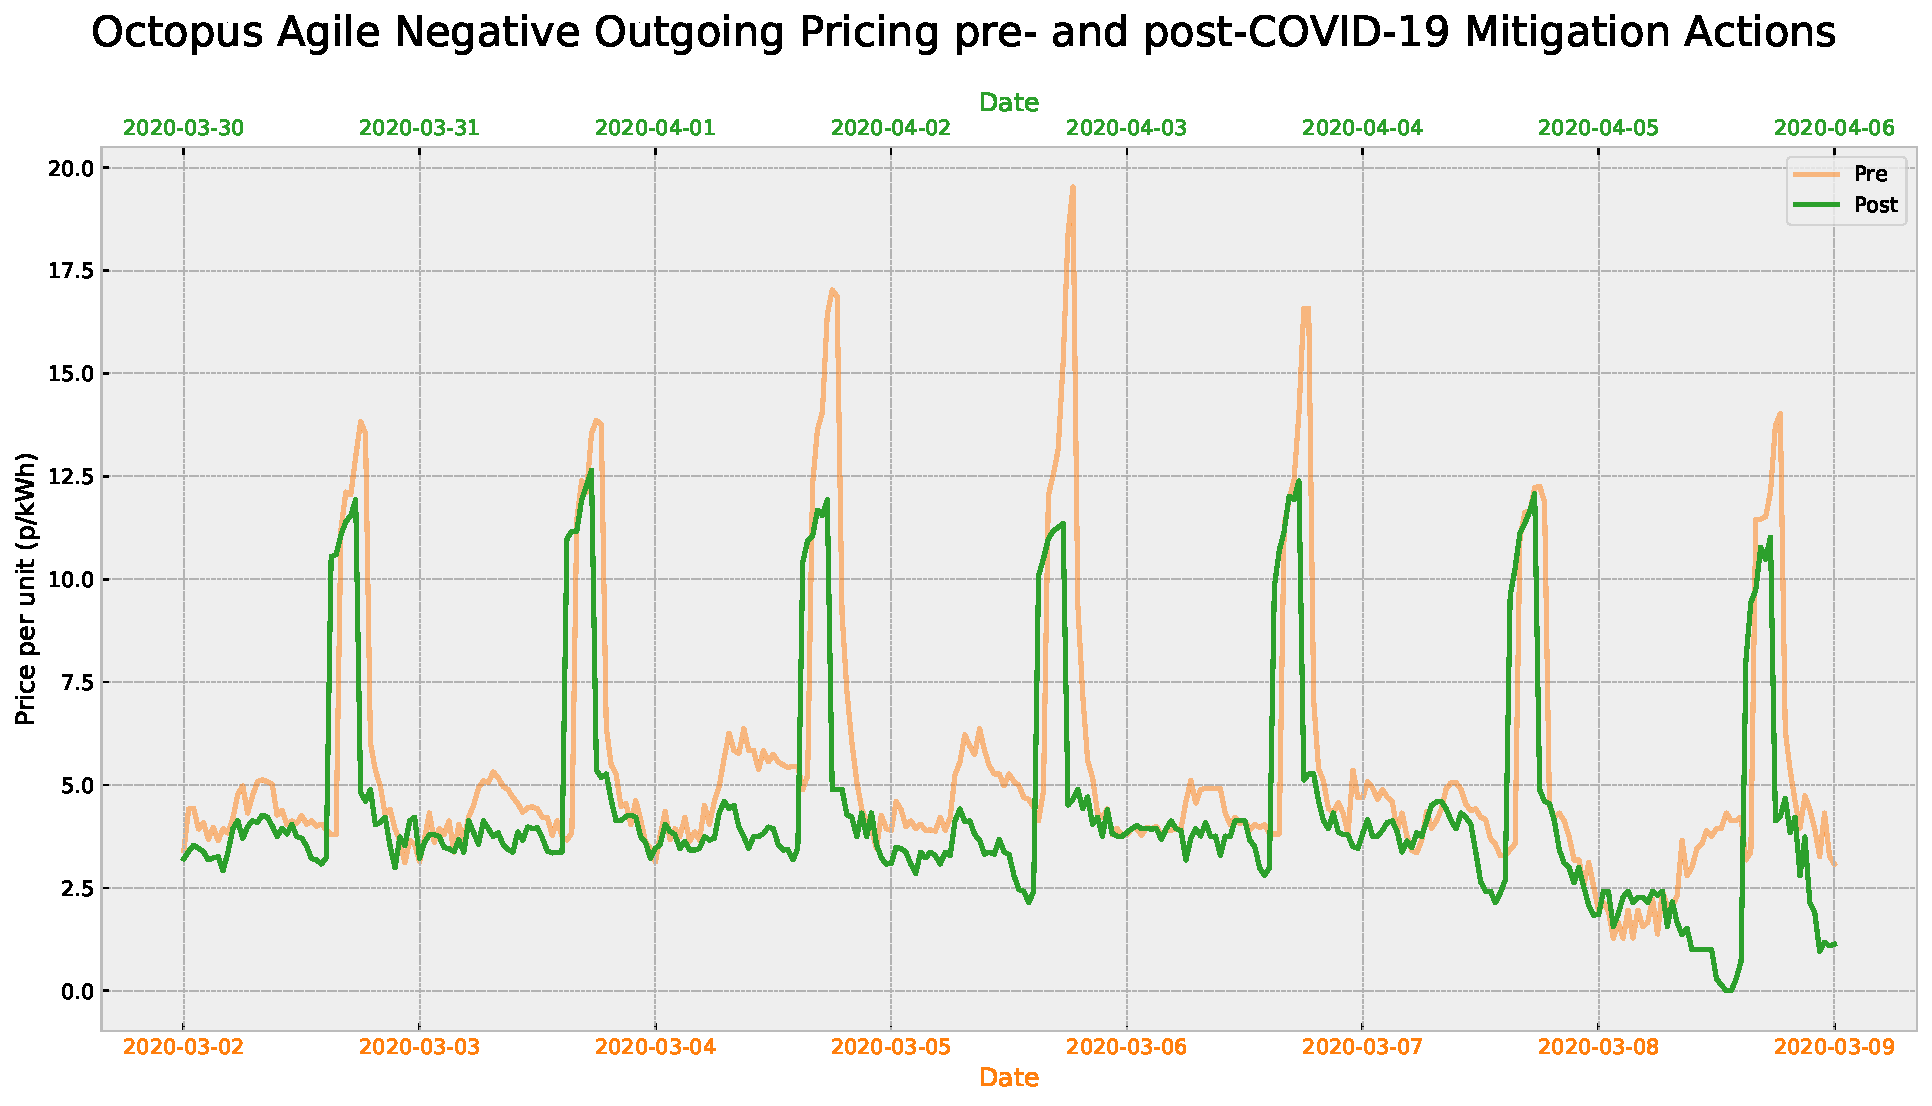
\includegraphics[width=15 cm]{Graphics/Pre-post_AgileOUTGO_negative_comp.pdf}
\caption{Corresponding Agile outgoing sell prices.}\label{fig:neg_agile_comp_prepost}
\end{figure}  

Since the launch of the Agile tariff, there has been 96 occurrences of negative pricing (i.e. price < 0p/kWh). Almost 70\% of these events (i.e. 67 out of 96) took place post-COVID-19 actions. Table \ref{table:neg_agile_table} summarises the pre and post negative pricing events highlighting the highest price the consumers were paid to use electricity and the corresponding dates.

\begin{table}[H]
\caption{Analysis of Negative Pricing usingthe  Agile Tariff data from Octopus \cite{AgileEnergy} }\label{table:neg_agile_table}
\centering
%% \tablesize{} %% You can specify the fontsize here, e.g., \tablesize{\footnotesize}. If commented out \small will be used.
\begin{tabular}{ccccc }
\toprule
\textbf{Data} & \textbf{Mean}	& \textbf{Min}	& \textbf{Max}& Dates corresponding to max values\\
\midrule
Pre	(p/kWh)	& -1.62			& -0.07         & -4.85 &09-12-2019\\
Post (p/kWh) & -1.36			& -0.02         & -3.99& 20-04-2020\\
Overall (p/kWh) & -1.44			& -0.02         & -4.85 &09-12-2019\\
\bottomrule
\end{tabular}
\end{table}


%===============================================================
%                           DISCUSSION
%===============================================================

\section{Discussion}

\textcolor{blue}{
NOTES from initial observations: Every day is a "weekend" -> Lower and delayed morning peak, lower evening peak - generally lower consumption.
\begin{itemize}
    \item System operator - Harder to predict the demand profile and peak - challenges the forecasting/predictive algorithms employed by National Grid
    \subitem Did the machine learning algorithms/predictive control/etc. see this coming?
    \item Aggregators and agents in DSR - may be making profit- due to these unforeseen changes in demand profile
    \item Generators - changes in scheduling - also not selling as much as they were promised as the demand decreased
    \item Industrial and Domestic consumers - paying less? - fixed term contracts?
    \item the impact of a shift from commercial and industrial load to largely domestic load
\end{itemize}}

\textcolor{blue}{
\begin{itemize}
    \item Due to the lower load caused by the lock-down, the average share of VRE increases in the power system. (important for discussion, as generally with higher VRE shares, i) prediction errors increase, ii) more ancillary services, iii) and the DA-clearance price decrease [already recognized from data])
\end{itemize}
}

\textcolor{blue}{
\begin{itemize}
    \item The head of the IEA, Fatih Birol, estimated that we are looking now one decade into the future power system, when the share of renewables is much more higher \cite{IgorTodorovic2020Birol:Balance}. This is not fully correct.
\end{itemize}
}

\subsection{Implications for Stakeholders}

The new disruptive and lower demand profile lead to multiple effects on stakeholders in the electricity system. The network operators will see on average increasing activation of balancing services to guarantee a reliable and stable grid and lower network loads. First, higher amount of balancing services can be explained due to the observed performance drop in short-term forecasting (see Section \ref{DemandForecastError}). Secondly, although, some network sections will lower in load due to the reasonable lower average demand in GB, some other network section could increase in loading as centralised renewable energy sources will transport energy for longer distances. The reason for longer transported energy is the lower electricity consumption closer to the VRE generators. For instance, the massive wind capacities installed in Great Britain's North - Scotland, providing energy up the southern part - London; when the net consumption in GB decreases, less energy will be directly consumed in the north and lead finally to higher network loads along the transmission lines at high wind and solar times. Therefore, even when the load in most networks will decrease some might also experience the contrary.

In the wholesale market, customer (Supplier) enter contracts with producer (Generators) which form together a Balancing and Settlement Code party \cite{ELEXON2019GuidanceBritain}. Since the imbalance due to rising load uncertainty increases, these parties are more often faced to imbalance charges towards the system operator. The trend of the total amount of imbalance charges cannot be easily detected, as described in Section \ref{sec:system imbalance price}, imbalance pricing is a complex measure which can increase and decrease due to the lock-down effects. 

Beside the imbalance, generators and suppliers, will suffer from the disruptive demand change in terms of profitability. The share of fix-cost compared to amount of sales will increase, leading eventually to higher electricity prices for domestic and industrial consumers. Otherwise, energy intensive companies which can directly participate on the electricity market can benefit from lower wholesale electricity prices (see Section \ref{sec:day-ahead wholesale market price}).

Aggregators and Demand side response (DSR) providers are expected to be more often scheduled because of the larger imbalance volume observed after the lock-down. The only requirement for them is to be more competitive then the new entering flexibility's from the non-scheduled power plants. If so, aggregators and DSR providers will benefit from the COVID-19 crisis.

\begin{figure}[H]
\centering
\hspace{-25pt}
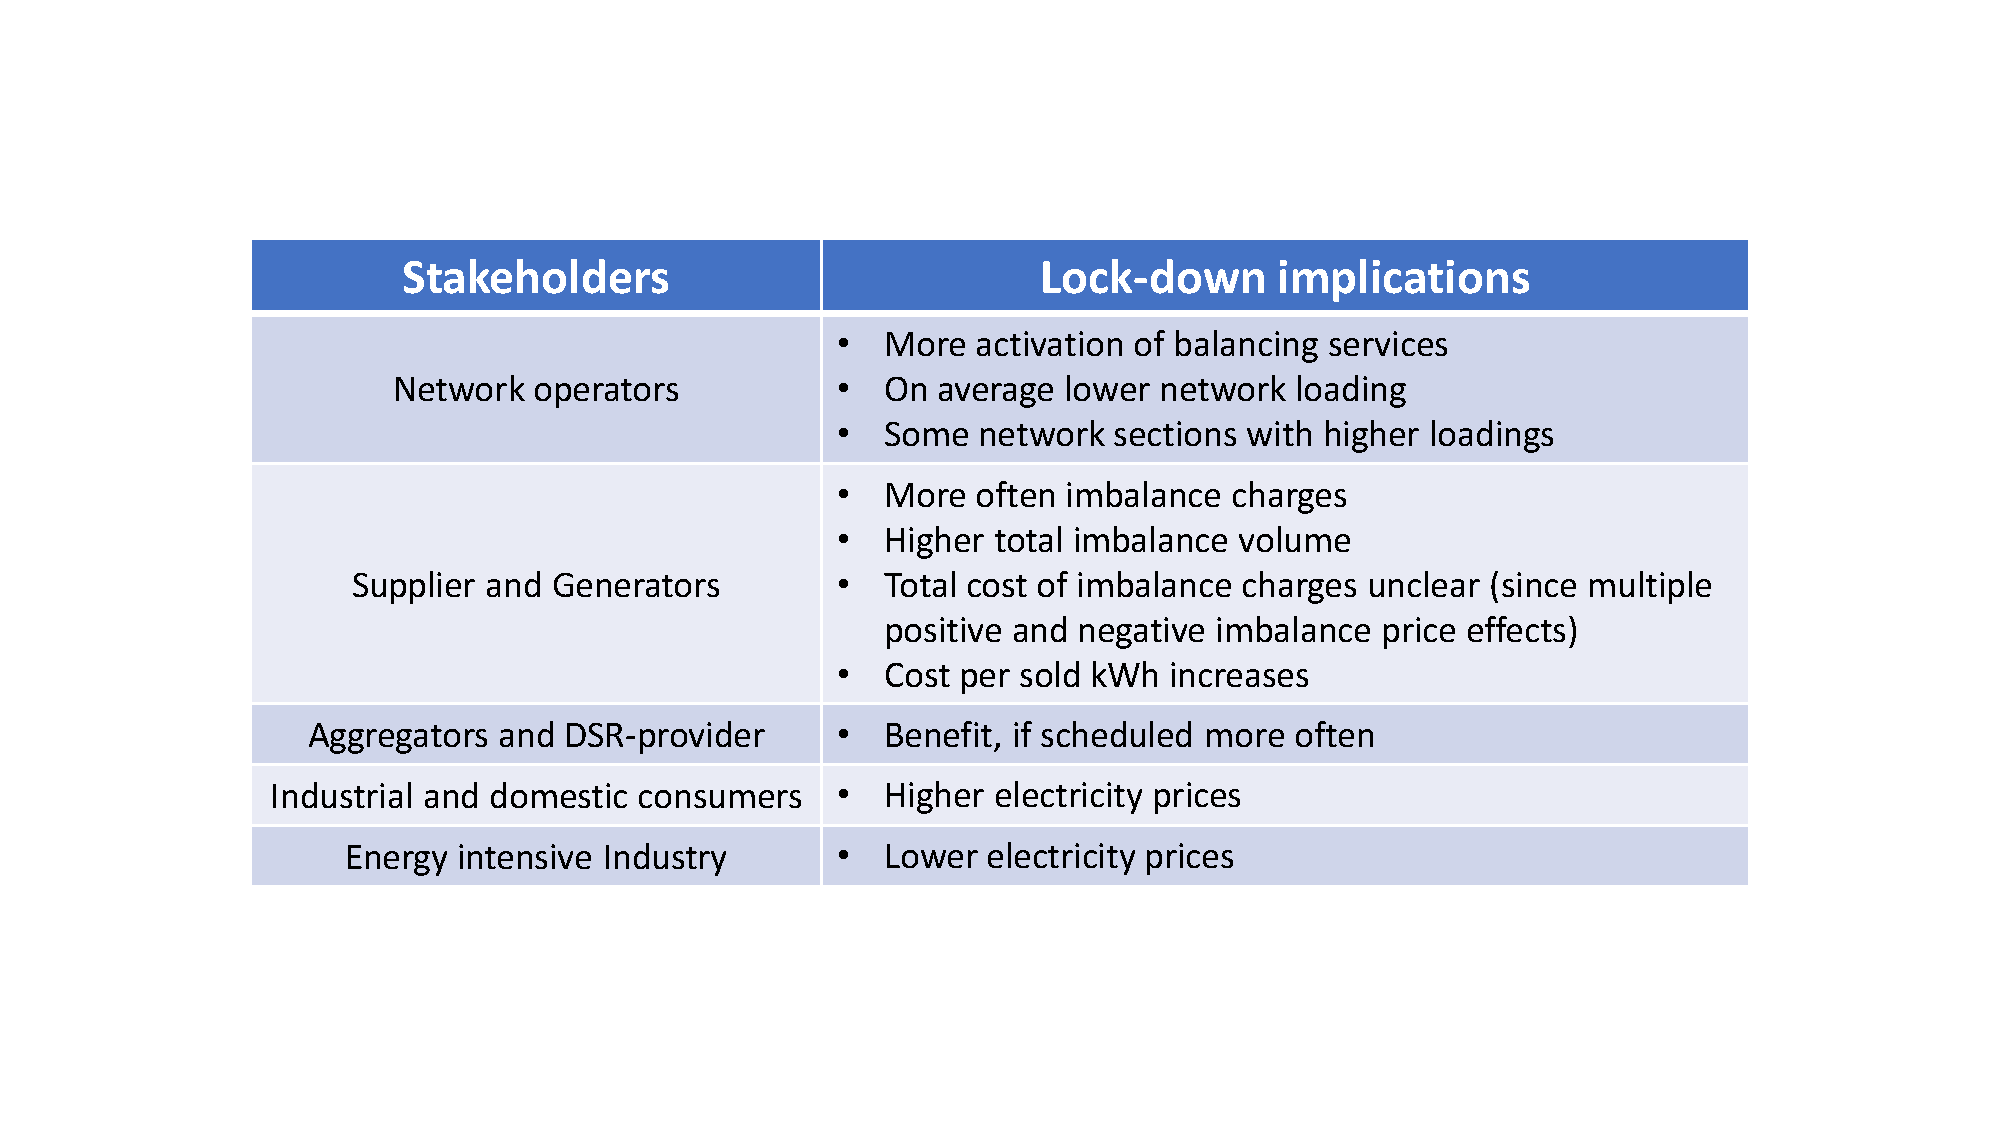
\includegraphics[trim={2cm 3cm 2cm 3.5cm},clip,width=1\textwidth]{Graphics/Stakeholder - lock-down implications.pdf}
\caption{The implication of the lock-down on the various stakeholders}
\label{fig:imbalance-price-trade-off}
\end{figure} 



%===============================================================
%                           CONCLUSIONS
%===============================================================
\section{Conclusions}

This section is not mandatory, but can be added to the manuscript if the discussion is unusually long or complex.
*copy from intro
*summarise contributions
***This paper encourage further research***

\vspace{6pt} 

%===============================================================
%                           MISC
%===============================================================

%%%%%%%%%%%%%%%%%%%%%%%%%%%%%%%%%%%%%%%%%%
%% optional
%\supplementary{The following are available online at \linksupplementary{s1}, Figure S1: title, Table S1: title, Video S1: title.}

%%%%%%%%%%%%%%%%%%%%%%%%%%%%%%%%%%%%%%%%%%
\authorcontributions{For research articles with several authors, a short paragraph specifying their individual contributions must be provided. The following statements should be used ``conceptualization, X.X. and Y.Y.; methodology, X.X.; software, X.X.; validation, X.X., Y.Y. and Z.Z.; formal analysis, X.X.; investigation, X.X.; resources, X.X.; data curation, X.X.; writing--original draft preparation, X.X.; writing--review and editing, X.X.; visualization, X.X.; supervision, X.X.; project administration, X.X.; funding acquisition, Y.Y.'', please turn to the  \href{http://img.mdpi.org/data/contributor-role-instruction.pdf}{CRediT taxonomy} for the term explanation. Authorship must be limited to those who have contributed substantially to the work reported.}

%%%%%%%%%%%%%%%%%%%%%%%%%%%%%%%%%%%%%%%%%%
\funding{Please add: ``This research received no external funding'' or ``This research was funded by NAME OF FUNDER grant number XXX.'' and  and ``The APC was funded by XXX''. Check carefully that the details given are accurate and use the standard spelling of funding agency names at \url{https://search.crossref.org/funding}, any errors may affect your future funding.}

%%%%%%%%%%%%%%%%%%%%%%%%%%%%%%%%%%%%%%%%%%
\acknowledgments{In this section you can acknowledge any support given which is not covered by the author contribution or funding sections. This may include administrative and technical support, or donations in kind (e.g., materials used for experiments).}

%%%%%%%%%%%%%%%%%%%%%%%%%%%%%%%%%%%%%%%%%%
\conflictsofinterest{The authors declare no conflict of interest. The funders had no role in the design of the study; in the collection, analyses, or interpretation of data; in the writing of the manuscript, or in the decision to publish the results.} 

%%%%%%%%%%%%%%%%%%%%%%%%%%%%%%%%%%%%%%%%%%
%% optional
\abbreviations{The following abbreviations are used in this manuscript:\\

\noindent 
\begin{tabular}{@{}ll}
MDPI & Multidisciplinary Digital Publishing Institute\\
DOAJ & Directory of open access journals\\
TLA & Three letter acronym\\
LD & linear dichroism
\end{tabular}}

%%%%%%%%%%%%%%%%%%%%%%%%%%%%%%%%%%%%%%%%%%
%% optional
\appendixtitles{no} %Leave argument "no" if all appendix headings stay EMPTY (then no dot is printed after "Appendix A"). If the appendix sections contain a heading then change the argument to "yes".
\appendix
\section{Agile Tariff}

\begin{figure}[H]
\centering
\hspace{-25pt}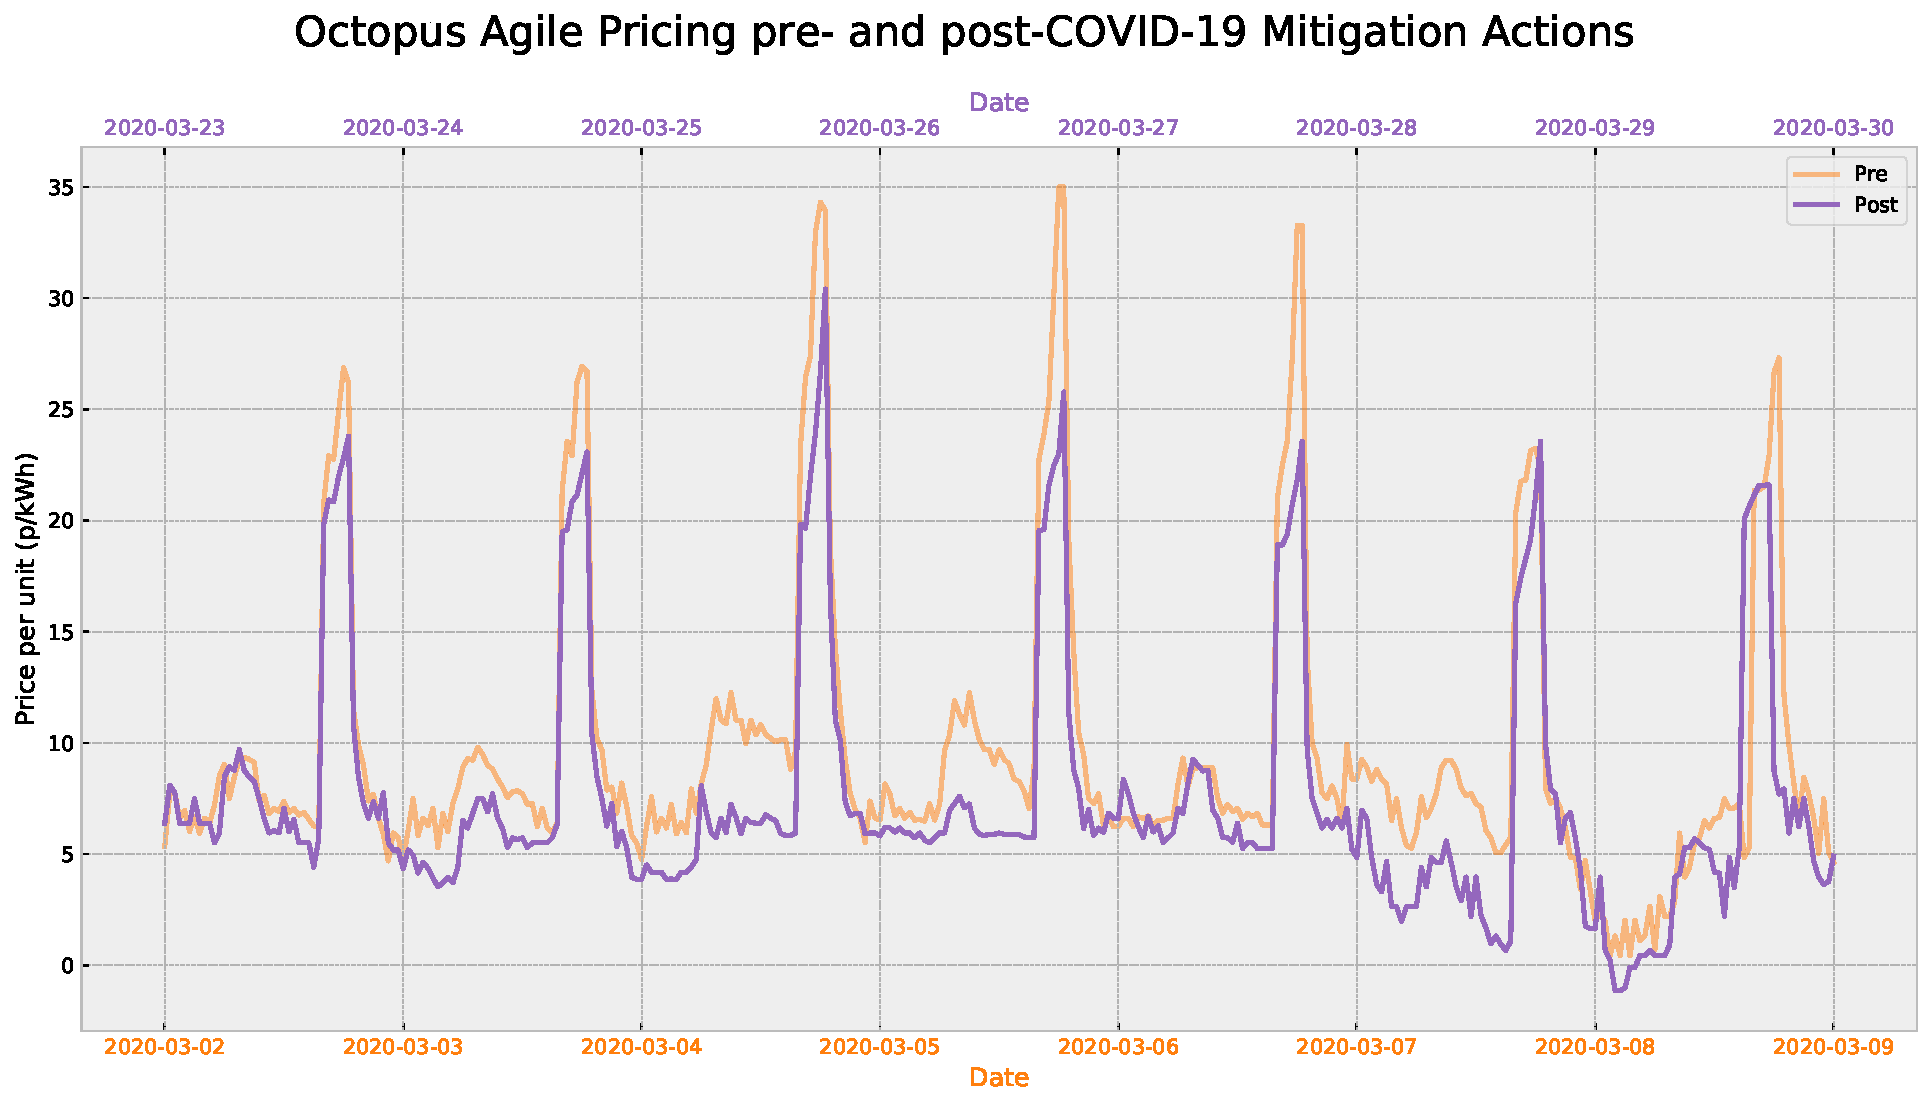
\includegraphics[width=15 cm]{Graphics/Pre-post_Agilecomp.pdf}
\caption{Octopus Agile Pricing comparison of before and after the COVID-19 actions.}\label{fig:agile_comp_prepost}
\end{figure}

\begin{figure}[H]\centering
\hspace{-25pt}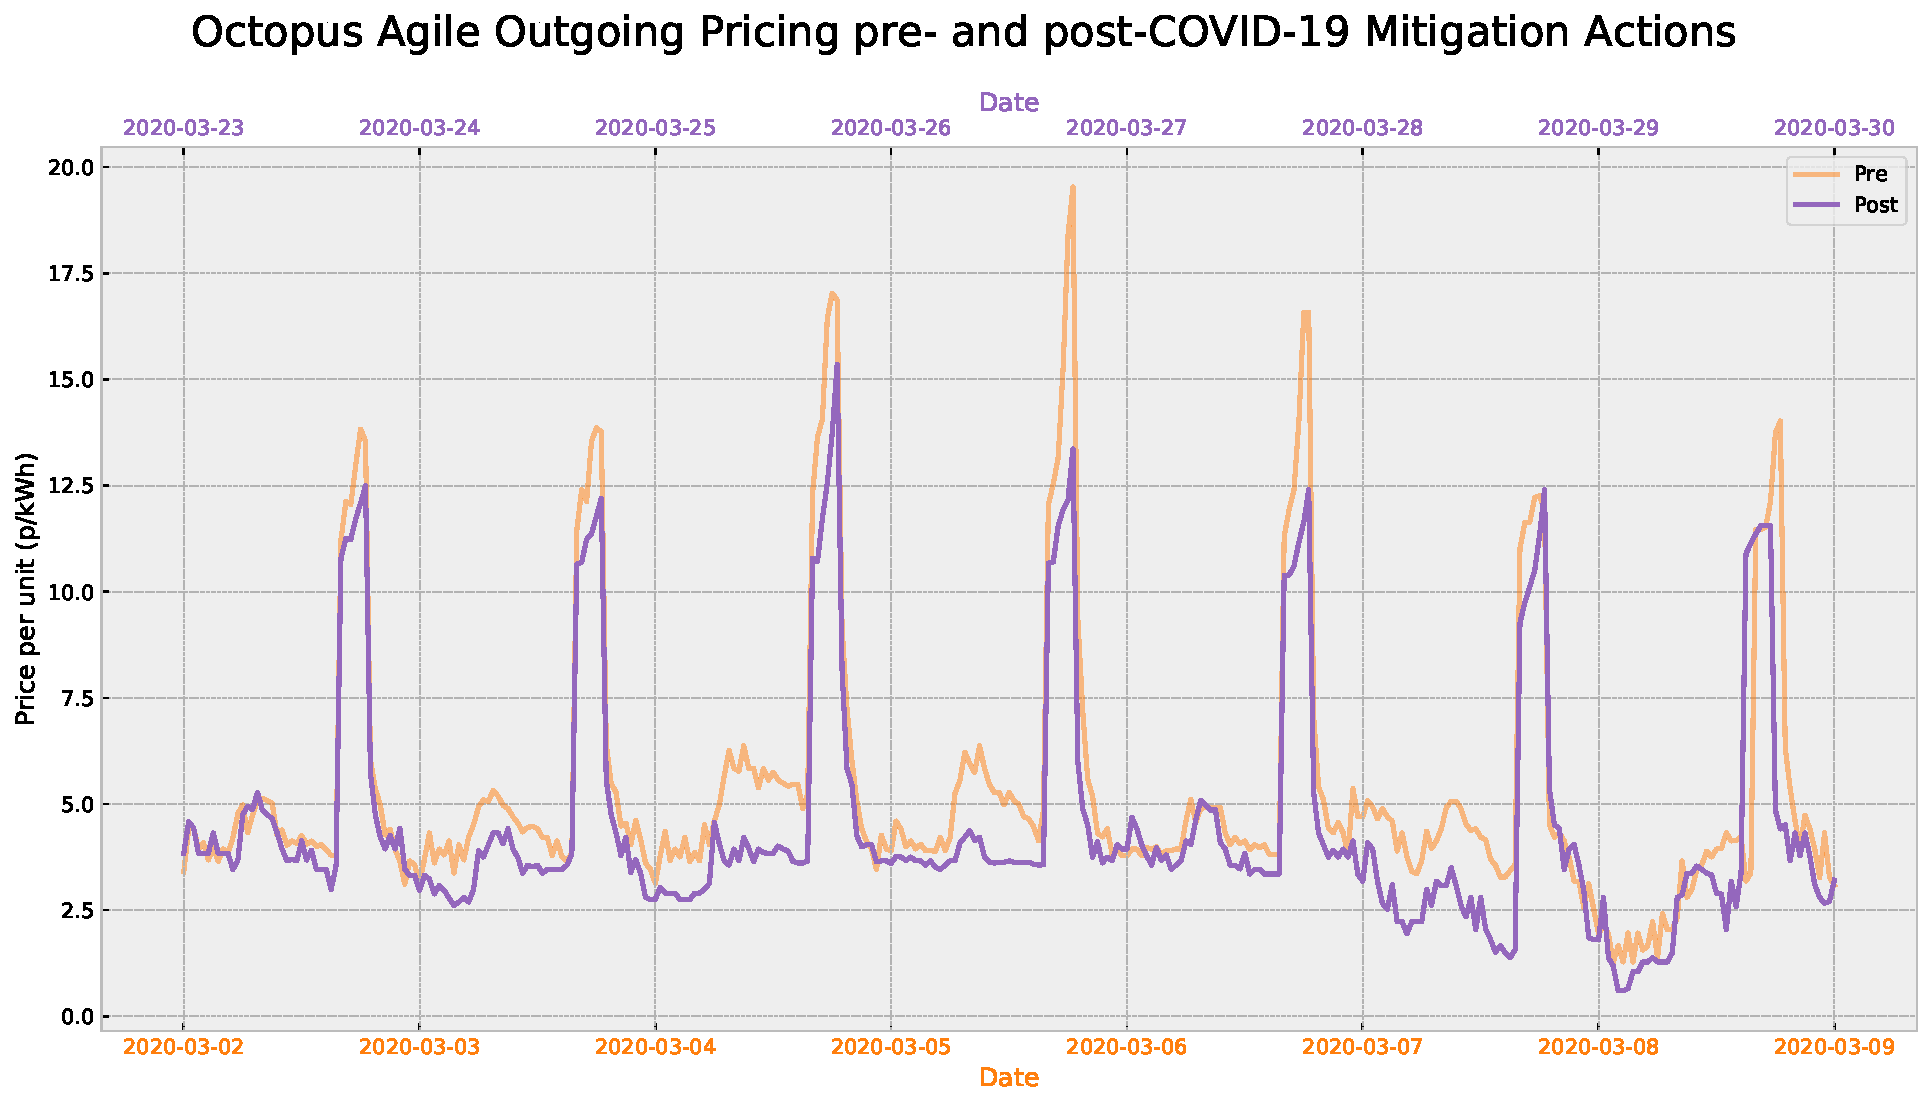
\includegraphics[width=15 cm]{Graphics/Pre-post_AgileOUTGO_comp.pdf}
\caption{Octopus Agile sell pricing comparison of before and after the COVID-19 actions.}\label{fig:agile_OUT_comp_prepost}
\end{figure}  
\section{LOLP \& DRM}

\begin{figure}[H]\centering
\hspace{-25pt}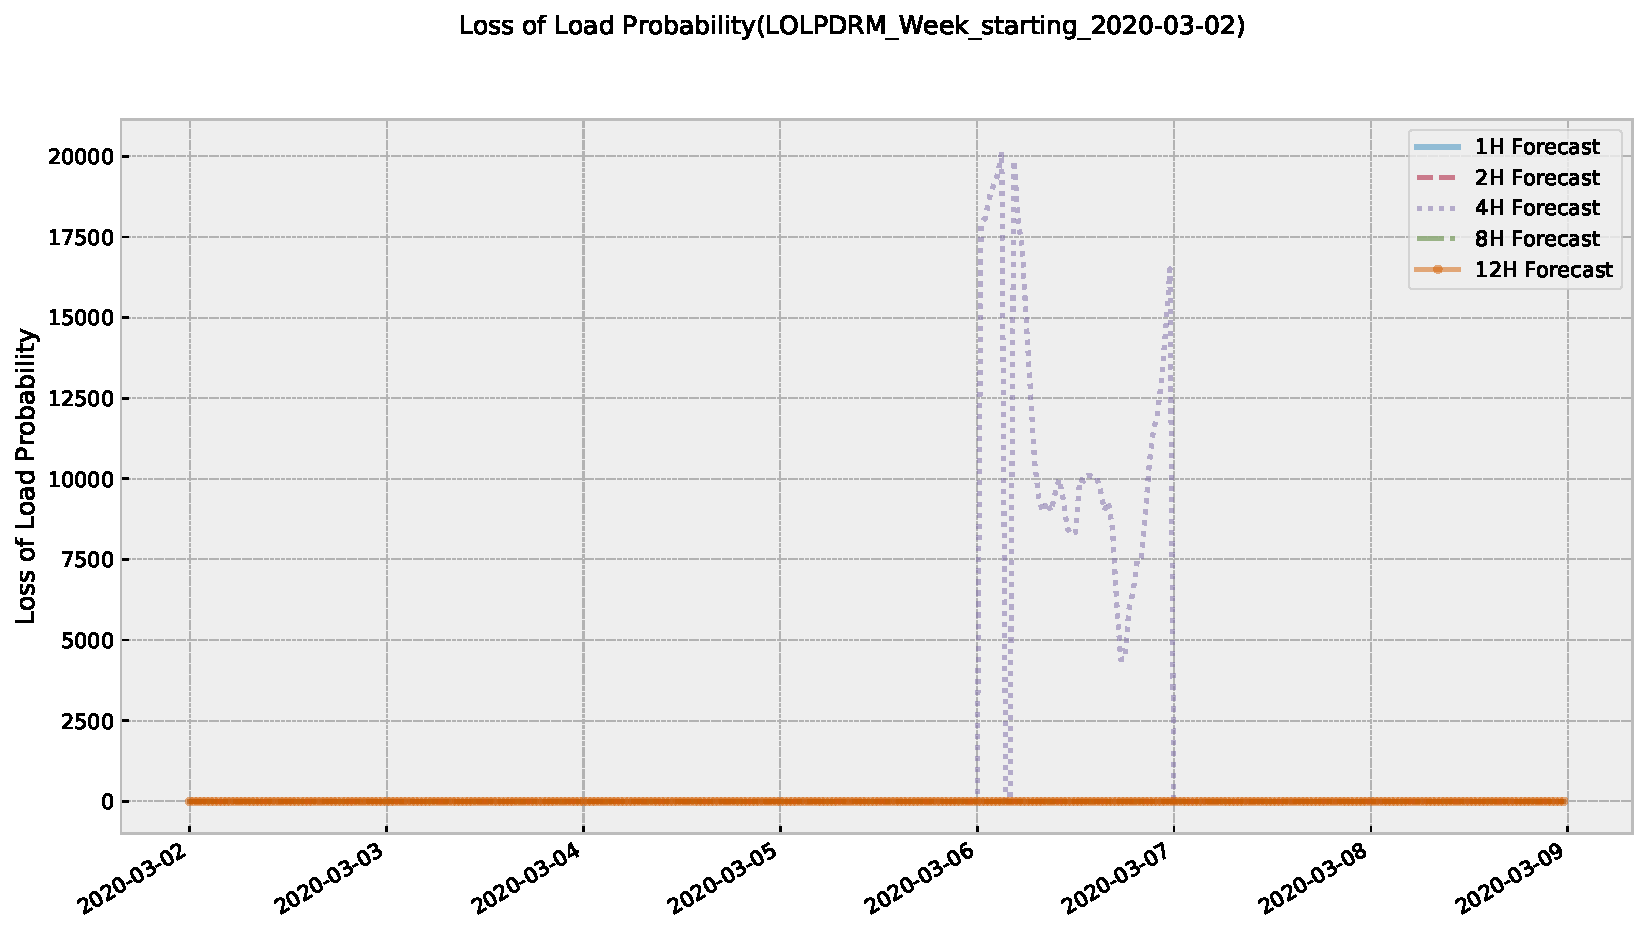
\includegraphics[width=15 cm]{Graphics/LOLPDRM_Week_starting_2020-03-02.pdf}
\caption{}\label{}
\end{figure}  
\begin{figure}[H]\centering
\hspace{-25pt}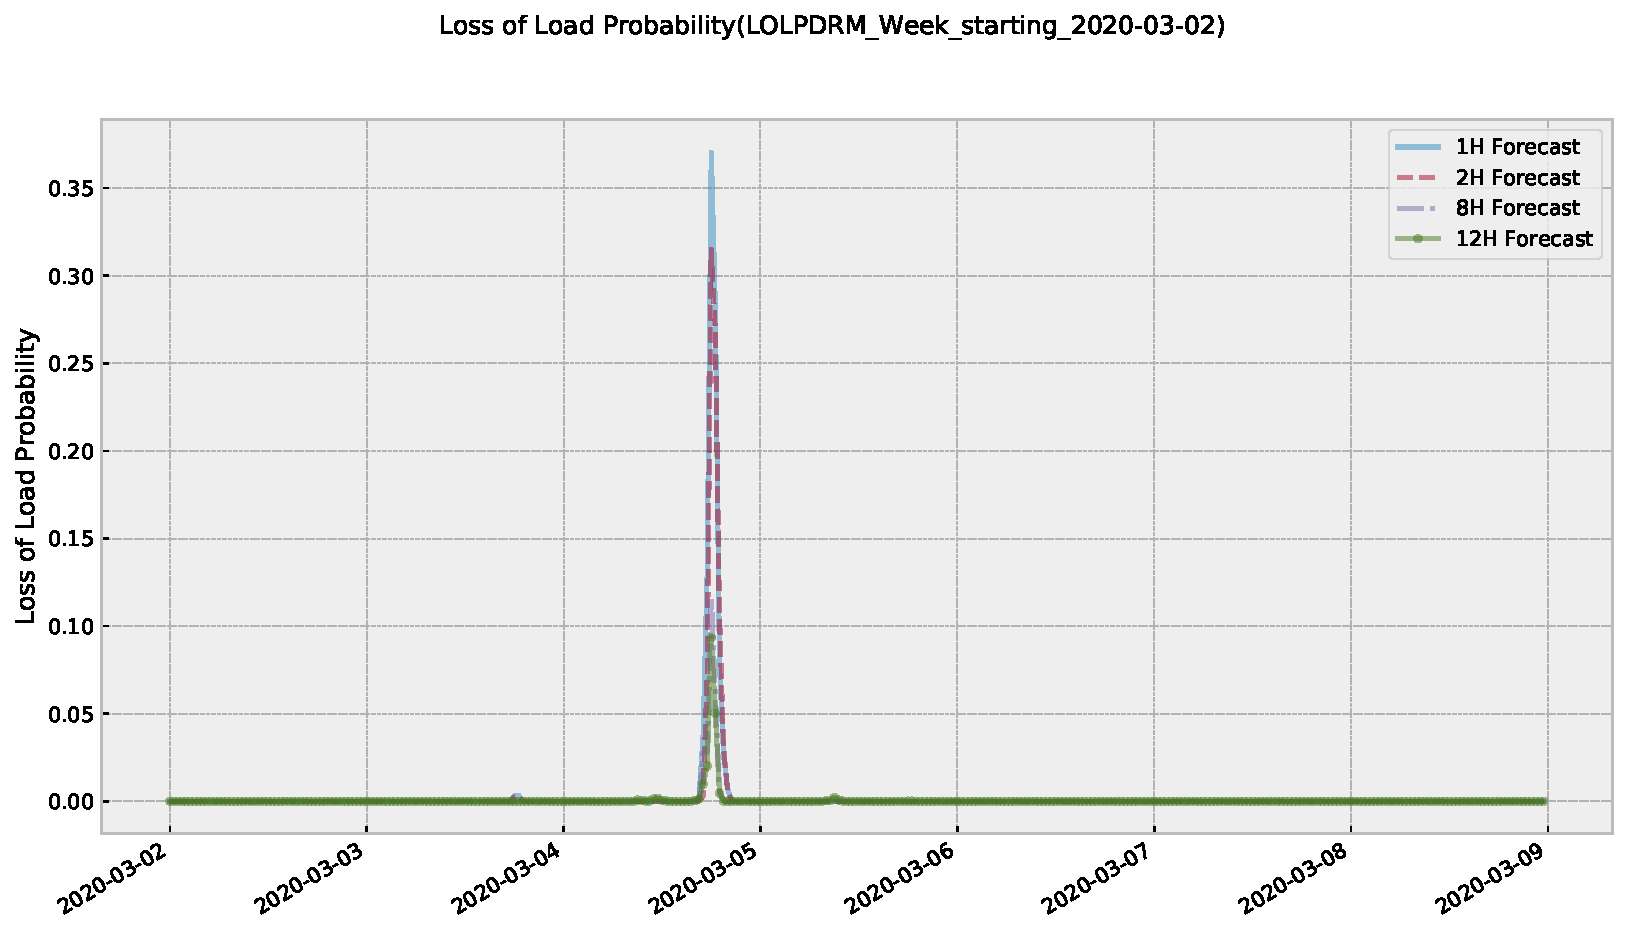
\includegraphics[width=15 cm]{Graphics/LOLPDRM_Week_starting_2020-03-02no4H.pdf}
\caption{}\label{}
\end{figure}  
\begin{figure}[H]\centering
\hspace{-25pt}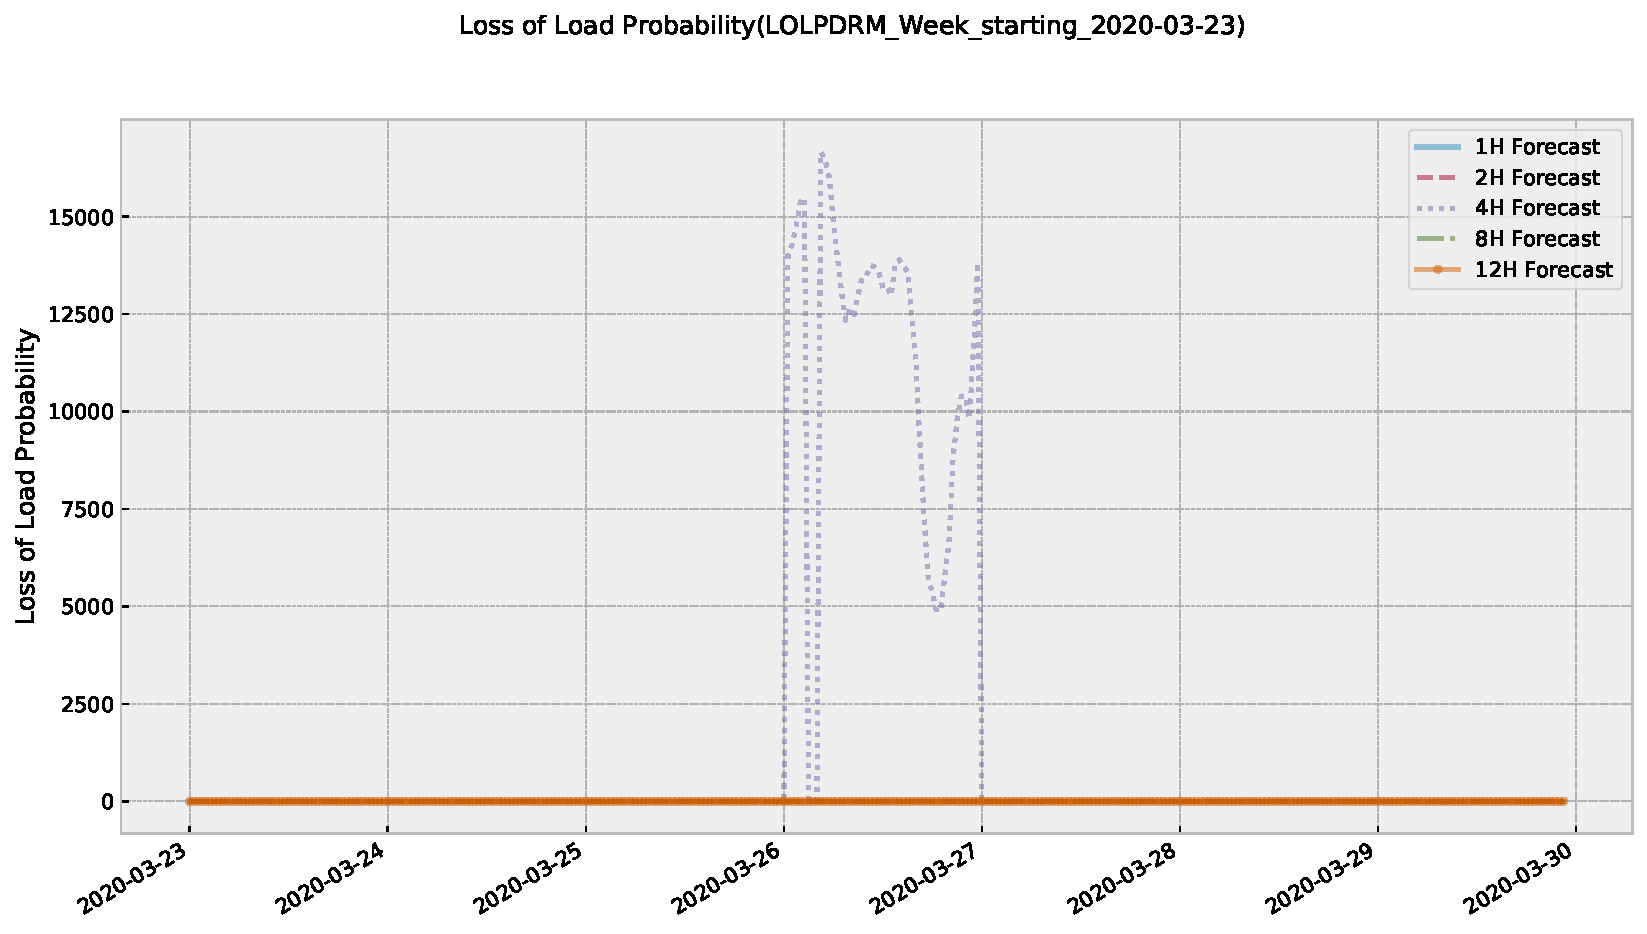
\includegraphics[width=15 cm]{Graphics/LOLPDRM_Week_starting_2020-03-23.pdf}
\caption{}\label{}
\end{figure}  
\begin{figure}[H]\centering
\hspace{-25pt}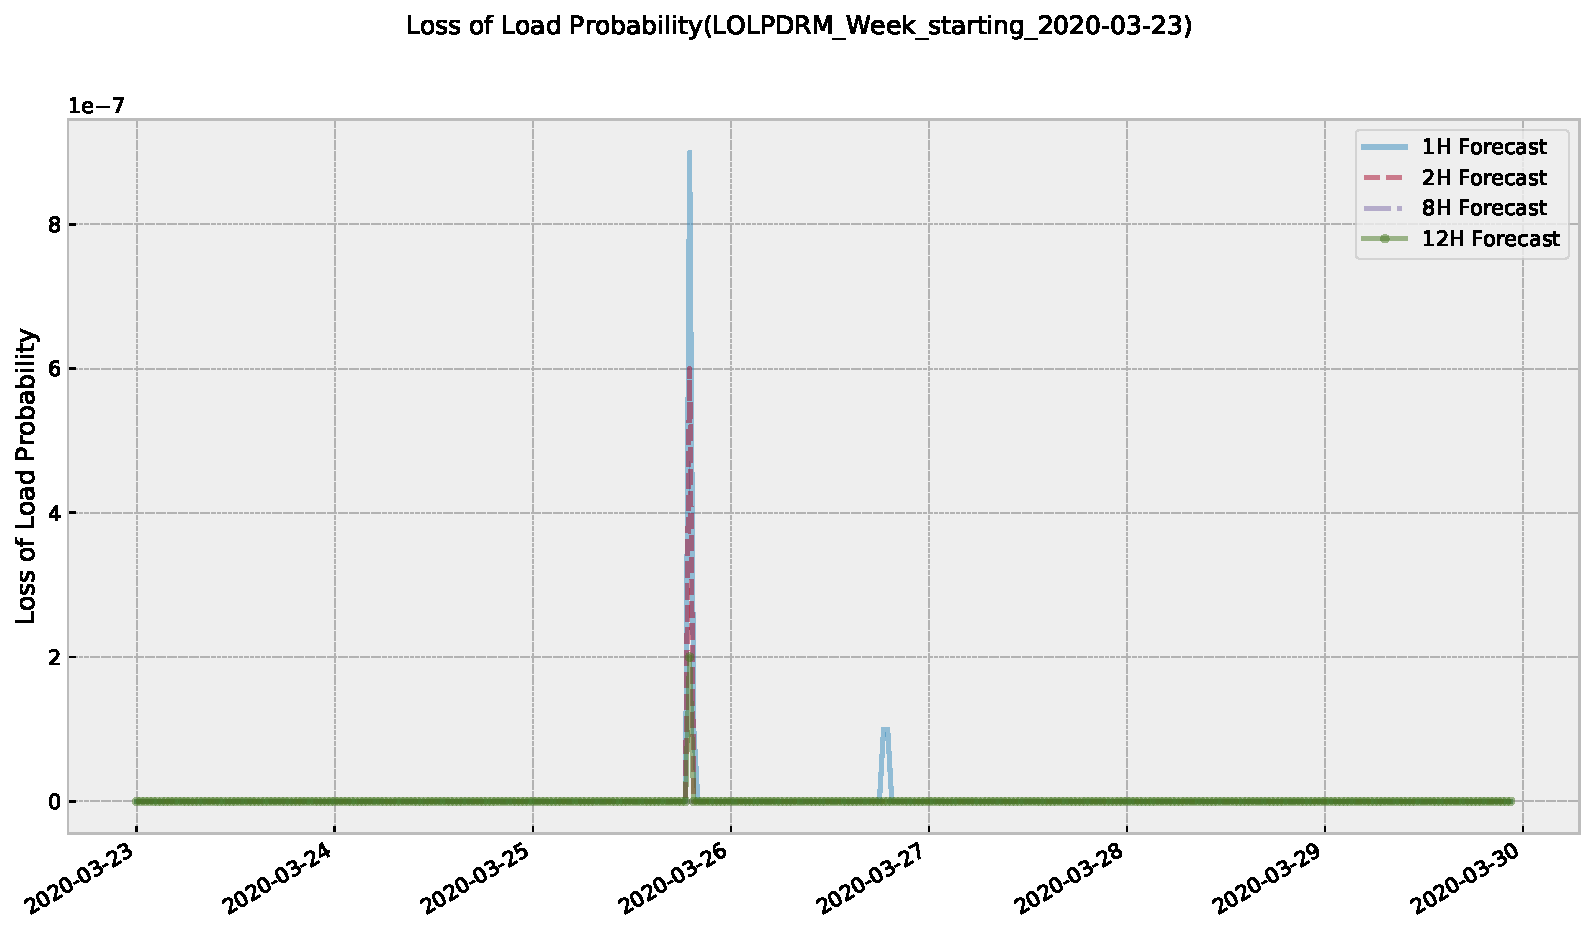
\includegraphics[width=15 cm]{Graphics/LOLPDRM_Week_starting_2020-03-23no4H.pdf}
\caption{}\label{}
\end{figure}  



\unskip
\subsection{}
The appendix is an optional section that can contain details and data supplemental to the main text. For example, explanations of experimental details that would disrupt the flow of the main text, but nonetheless remain crucial to understanding and reproducing the research shown; figures of replicates for experiments of which representative data is shown in the main text can be added here if brief, or as Supplementary data. Mathematical proofs of results not central to the paper can be added as an appendix.


%===============================================================
%                           REFERENCES
%===============================================================

\reftitle{References}

\externalbibliography{yes}
\bibliography{references.bib}
\bibliography{referencesmax.bib}
%%%%%%%%%%%%%%%%%%%%%%%%%%%%%%%%%%%%%%%%%%
%% optional
% \sampleavailability{Samples of the compounds ...... are available from the authors.}

%% for journal Sci
%\reviewreports{\\
%Reviewer 1 comments and authors’ response\\
%Reviewer 2 comments and authors’ response\\
%Reviewer 3 comments and authors’ response
%}

%%%%%%%%%%%%%%%%%%%%%%%%%%%%%%%%%%%%%%%%%%
\end{document}



% \begin{thebibliography}{999}
% % Reference 1
% \bibitem[Author1(year)]{ref-journal}
% Author1, T. The title of the cited article. {\em Journal Abbreviation} {\bf 2008}, {\em 10}, 142--149.
% % Reference 2
% \bibitem[Author2(year)]{ref-book}
% Author2, L. The title of the cited contribution. In {\em The Book Title}; Editor1, F., Editor2, A., Eds.; Publishing House: City, Country, 2007; pp. 32--58.
% \end{thebibliography}


% To cite two works by the same author: \citeauthor{ref-journal-1a} (\citeyear{ref-journal-1a}, \citeyear{ref-journal-1b}). This produces: Whittaker (1967, 1975)
% To cite two works by the same author with specific pages: \citeauthor{ref-journal-3a} (\citeyear{ref-journal-3a}, p. 328; \citeyear{ref-journal-3b}, p.475). This produces: Wong (1999, p. 328; 2000, p. 475)

%=====================================
% References, variant B: external bibliography
%=====================================


% \section{Results}

% This section may be divided by subheadings. It should provide a concise and precise description of the experimental results, their interpretation as well as the experimental conclusions that can be drawn.
% \begin{quote}
% This section may be divided by subheadings. It should provide a concise and precise description of the experimental results, their interpretation as well as the experimental conclusions that can be drawn.
% \end{quote}

% %%%%%%%%%%%%%%%%%%%%%%%%%%%%%%%%%%%%%%%%%%
% \subsection{Subsection}
% \unskip
% \subsubsection{Subsubsection}

% Bulleted lists look like this:
% \begin{itemize}[leftmargin=*,labelsep=5.8mm]
% \item	First bullet
% \item	Second bullet
% \item	Third bullet
% \end{itemize}

% Numbered lists can be added as follows:
% \begin{enumerate}[leftmargin=*,labelsep=4.9mm]
% \item	First item 
% \item	Second item
% \item	Third item
% \end{enumerate}

% The text continues here.

% \subsection{Figures, Tables and Schemes}

% All figures and tables should be cited in the main text as Figure 1, Table 1, etc.

% \begin{figure}[H]
% \centering
% 
\includegraphics[width=2 cm]{Definitions/logo-mdpi}
% \caption{This is a figure, Schemes follow the same formatting. If there are multiple panels, they should be listed as: (\textbf{a}) Description of what is contained in the first panel. (\textbf{b}) Description of what is contained in the second panel. Figures should be placed in the main text near to the first time they are cited. A caption on a single line should be centered.}
% \end{figure}   
 
% Text

% Text

% \begin{table}[H]
% \caption{This is a table caption. Tables should be placed in the main text near to the first time they are cited.}
% \centering
% %% \tablesize{} %% You can specify the fontsize here, e.g., \tablesize{\footnotesize}. If commented out \small will be used.
% \begin{tabular}{ccc}
% \toprule
% \textbf{Title 1}	& \textbf{Title 2}	& \textbf{Title 3}\\
% \midrule
% entry 1		& data			& data\\
% entry 2		& data			& data\\
% \bottomrule
% \end{tabular}
% \end{table}

% Text

% Text

% %\begin{listing}[H]
% %\caption{Title of the listing}
% %\rule{\textwidth}{1pt}
% %\raggedright Text of the listing. In font size footnotesize, small, or normalsize. Preferred format: left aligned and single spaced. Preferred border format: top border line and bottom border line.
% %\rule{\textwidth}{1pt}
% %\end{listing}


% \subsection{Formatting of Mathematical Components}

% This is an example of an equation:

% \begin{equation}
% a + b = c
% \end{equation}
% %% If the documentclass option "submit" is chosen, please insert a blank line before and after any math environment (equation and eqnarray environments). This ensures correct linenumbering. The blank line should be removed when the documentclass option is changed to "accept" because the text following an equation should not be a new paragraph. 

% Please punctuate equations as regular text. Theorem-type environments (including propositions, lemmas, corollaries etc.) can be formatted as follows:
% %% Example of a theorem:
% \begin{Theorem}
% Example text of a theorem.
% \end{Theorem}

% The text continues here. Proofs must be formatted as follows:

% %% Example of a proof:
% \begin{proof}[Proof of Theorem 1]
% Text of the proof. Note that the phrase `of Theorem 1' is optional if it is clear which theorem is being referred to.
% \end{proof}
% The text continues here.

% %%%%%%%%%%%%%%%%%%%%%%%%%%%%%%%%%%%%%%%%%%
% \section{Discussion}

% Authors should discuss the results and how they can be interpreted in perspective of previous studies and of the working hypotheses. The findings and their implications should be discussed in the broadest context possible. Future research directions may also be highlighted.

% %%%%%%%%%%%%%%%%%%%%%%%%%%%%%%%%%%%%%%%%%%
% \section{Materials and Methods}

% Materials and Methods should be described with sufficient details to allow others to replicate and build on published results. Please note that publication of your manuscript implicates that you must make all materials, data, computer code, and protocols associated with the publication available to readers. Please disclose at the submission stage any restrictions on the availability of materials or information. New methods and protocols should be described in detail while well-established methods can be briefly described and appropriately cited.

% Research manuscripts reporting large datasets that are deposited in a publicly available database should specify where the data have been deposited and provide the relevant accession numbers. If the accession numbers have not yet been obtained at the time of submission, please state that they will be provided during review. They must be provided prior to publication.

% Interventionary studies involving animals or humans, and other studies require ethical approval must list the authority that provided approval and the corresponding ethical approval code. 